\documentclass[twoside]{book}

% Packages required by doxygen
\usepackage{calc}
\usepackage{doxygen}
\usepackage{graphicx}
\usepackage[utf8]{inputenc}
\usepackage{makeidx}
\usepackage{multicol}
\usepackage{multirow}
\usepackage{textcomp}
\usepackage[table]{xcolor}

% Font selection
\usepackage[T1]{fontenc}
\usepackage{mathptmx}
\usepackage[scaled=.90]{helvet}
\usepackage{courier}
\usepackage{amssymb}
\usepackage{sectsty}
\renewcommand{\familydefault}{\sfdefault}
\allsectionsfont{%
  \fontseries{bc}\selectfont%
  \color{darkgray}%
}
\renewcommand{\DoxyLabelFont}{%
  \fontseries{bc}\selectfont%
  \color{darkgray}%
}

% Page & text layout
\usepackage{geometry}
\geometry{%
  a4paper,%
  top=2.5cm,%
  bottom=2.5cm,%
  left=2.5cm,%
  right=2.5cm%
}
\tolerance=750
\hfuzz=15pt
\hbadness=750
\setlength{\emergencystretch}{15pt}
\setlength{\parindent}{0cm}
\setlength{\parskip}{0.2cm}
\makeatletter
\renewcommand{\paragraph}{%
  \@startsection{paragraph}{4}{0ex}{-1.0ex}{1.0ex}{%
    \normalfont\normalsize\bfseries\SS@parafont%
  }%
}
\renewcommand{\subparagraph}{%
  \@startsection{subparagraph}{5}{0ex}{-1.0ex}{1.0ex}{%
    \normalfont\normalsize\bfseries\SS@subparafont%
  }%
}
\makeatother

% Headers & footers
\usepackage{fancyhdr}
\pagestyle{fancyplain}
\fancyhead[LE]{\fancyplain{}{\bfseries\thepage}}
\fancyhead[CE]{\fancyplain{}{}}
\fancyhead[RE]{\fancyplain{}{\bfseries\leftmark}}
\fancyhead[LO]{\fancyplain{}{\bfseries\rightmark}}
\fancyhead[CO]{\fancyplain{}{}}
\fancyhead[RO]{\fancyplain{}{\bfseries\thepage}}
\fancyfoot[LE]{\fancyplain{}{}}
\fancyfoot[CE]{\fancyplain{}{}}
\fancyfoot[RE]{\fancyplain{}{\bfseries\scriptsize Generated on Mon May 14 2018 19:20:09 for CS1C Class project - ERKK by Doxygen }}
\fancyfoot[LO]{\fancyplain{}{\bfseries\scriptsize Generated on Mon May 14 2018 19:20:09 for CS1C Class project - ERKK by Doxygen }}
\fancyfoot[CO]{\fancyplain{}{}}
\fancyfoot[RO]{\fancyplain{}{}}
\renewcommand{\footrulewidth}{0.4pt}
\renewcommand{\chaptermark}[1]{%
  \markboth{#1}{}%
}
\renewcommand{\sectionmark}[1]{%
  \markright{\thesection\ #1}%
}

% Indices & bibliography
\usepackage{natbib}
\usepackage[titles]{tocloft}
\setcounter{tocdepth}{3}
\setcounter{secnumdepth}{5}
\makeindex

% Hyperlinks (required, but should be loaded last)
\usepackage{ifpdf}
\ifpdf
  \usepackage[pdftex,pagebackref=true]{hyperref}
\else
  \usepackage[ps2pdf,pagebackref=true]{hyperref}
\fi
\hypersetup{%
  colorlinks=true,%
  linkcolor=blue,%
  citecolor=blue,%
  unicode%
}

% Custom commands
\newcommand{\clearemptydoublepage}{%
  \newpage{\pagestyle{empty}\cleardoublepage}%
}


%===== C O N T E N T S =====

\begin{document}

% Titlepage & ToC
\hypersetup{pageanchor=false}
\pagenumbering{roman}
\begin{titlepage}
\vspace*{7cm}
\begin{center}%
{\Large C\-S1\-C Class project -\/ E\-R\-K\-K }\\
\vspace*{1cm}
{\large Generated by Doxygen 1.8.4}\\
\vspace*{0.5cm}
{\small Mon May 14 2018 19:20:09}\\
\end{center}
\end{titlepage}
\clearemptydoublepage
\tableofcontents
\clearemptydoublepage
\pagenumbering{arabic}
\hypersetup{pageanchor=true}

%--- Begin generated contents ---
\chapter{Hierarchical Index}
\section{Class Hierarchy}
This inheritance list is sorted roughly, but not completely, alphabetically\-:\begin{DoxyCompactList}
\item \contentsline{section}{compare\-\_\-shape\-\_\-area}{\pageref{structcompare__shape__area}}{}
\item \contentsline{section}{compare\-\_\-shape\-\_\-id}{\pageref{structcompare__shape__id}}{}
\item \contentsline{section}{compare\-\_\-shape\-\_\-perimeter}{\pageref{structcompare__shape__perimeter}}{}
\item \contentsline{section}{nserkkvector\-:\-:My\-Vector$<$ T $>$}{\pageref{classnserkkvector_1_1MyVector}}{}
\item \contentsline{section}{nserkkvector\-:\-:My\-Vector$<$ Shape $\ast$ $>$}{\pageref{classnserkkvector_1_1MyVector}}{}
\item Q\-Dialog\begin{DoxyCompactList}
\item \contentsline{section}{about}{\pageref{classabout}}{}
\item \contentsline{section}{contact}{\pageref{classcontact}}{}
\item \contentsline{section}{login}{\pageref{classlogin}}{}
\end{DoxyCompactList}
\item Q\-Main\-Window\begin{DoxyCompactList}
\item \contentsline{section}{Main\-Window}{\pageref{classMainWindow}}{}
\end{DoxyCompactList}
\item Q\-Object\begin{DoxyCompactList}
\item \contentsline{section}{privilege}{\pageref{classprivilege}}{}
\end{DoxyCompactList}
\item Q\-Widget\begin{DoxyCompactList}
\item \contentsline{section}{render\-Area}{\pageref{classrenderArea}}{}
\item \contentsline{section}{reports}{\pageref{classreports}}{}
\item \contentsline{section}{testimonials}{\pageref{classtestimonials}}{}
\end{DoxyCompactList}
\item \contentsline{section}{Shape}{\pageref{classShape}}{}
\begin{DoxyCompactList}
\item \contentsline{section}{Shape1\-D}{\pageref{classShape1D}}{}
\begin{DoxyCompactList}
\item \contentsline{section}{Line}{\pageref{classLine}}{}
\item \contentsline{section}{Poly\-Line}{\pageref{classPolyLine}}{}
\end{DoxyCompactList}
\item \contentsline{section}{Shape2\-D}{\pageref{classShape2D}}{}
\begin{DoxyCompactList}
\item \contentsline{section}{Circle}{\pageref{classCircle}}{}
\item \contentsline{section}{Ellipse}{\pageref{classEllipse}}{}
\item \contentsline{section}{Polygon}{\pageref{classPolygon}}{}
\item \contentsline{section}{Rectangle}{\pageref{classRectangle}}{}
\item \contentsline{section}{Square}{\pageref{classSquare}}{}
\end{DoxyCompactList}
\item \contentsline{section}{Text}{\pageref{classText}}{}
\end{DoxyCompactList}
\end{DoxyCompactList}

\chapter{Class Index}
\section{Class List}
Here are the classes, structs, unions and interfaces with brief descriptions\-:\begin{DoxyCompactList}
\item\contentsline{section}{\hyperlink{classabout}{about} }{\pageref{classabout}}{}
\item\contentsline{section}{\hyperlink{classCircle}{Circle} }{\pageref{classCircle}}{}
\item\contentsline{section}{\hyperlink{structcompare__shape__area}{compare\-\_\-shape\-\_\-area} }{\pageref{structcompare__shape__area}}{}
\item\contentsline{section}{\hyperlink{structcompare__shape__id}{compare\-\_\-shape\-\_\-id} }{\pageref{structcompare__shape__id}}{}
\item\contentsline{section}{\hyperlink{structcompare__shape__perimeter}{compare\-\_\-shape\-\_\-perimeter} }{\pageref{structcompare__shape__perimeter}}{}
\item\contentsline{section}{\hyperlink{classcontact}{contact} }{\pageref{classcontact}}{}
\item\contentsline{section}{\hyperlink{classEllipse}{Ellipse} }{\pageref{classEllipse}}{}
\item\contentsline{section}{\hyperlink{classLine}{Line} }{\pageref{classLine}}{}
\item\contentsline{section}{\hyperlink{classlogin}{login} }{\pageref{classlogin}}{}
\item\contentsline{section}{\hyperlink{classMainWindow}{Main\-Window} }{\pageref{classMainWindow}}{}
\item\contentsline{section}{\hyperlink{classnserkkvector_1_1MyVector}{nserkkvector\-::\-My\-Vector$<$ T $>$} }{\pageref{classnserkkvector_1_1MyVector}}{}
\item\contentsline{section}{\hyperlink{classPolygon}{Polygon} }{\pageref{classPolygon}}{}
\item\contentsline{section}{\hyperlink{classPolyLine}{Poly\-Line} }{\pageref{classPolyLine}}{}
\item\contentsline{section}{\hyperlink{classprivilege}{privilege} }{\pageref{classprivilege}}{}
\item\contentsline{section}{\hyperlink{classRectangle}{Rectangle} }{\pageref{classRectangle}}{}
\item\contentsline{section}{\hyperlink{classrenderArea}{render\-Area} }{\pageref{classrenderArea}}{}
\item\contentsline{section}{\hyperlink{classreports}{reports} }{\pageref{classreports}}{}
\item\contentsline{section}{\hyperlink{classShape}{Shape} }{\pageref{classShape}}{}
\item\contentsline{section}{\hyperlink{classShape1D}{Shape1\-D} }{\pageref{classShape1D}}{}
\item\contentsline{section}{\hyperlink{classShape2D}{Shape2\-D} }{\pageref{classShape2D}}{}
\item\contentsline{section}{\hyperlink{classSquare}{Square} }{\pageref{classSquare}}{}
\item\contentsline{section}{\hyperlink{classtestimonials}{testimonials} }{\pageref{classtestimonials}}{}
\item\contentsline{section}{\hyperlink{classText}{Text} }{\pageref{classText}}{}
\end{DoxyCompactList}

\chapter{Class Documentation}
\hypertarget{classabout}{\section{about Class Reference}
\label{classabout}\index{about@{about}}
}


{\ttfamily \#include $<$about.\-h$>$}

Inheritance diagram for about\-:\begin{figure}[H]
\begin{center}
\leavevmode
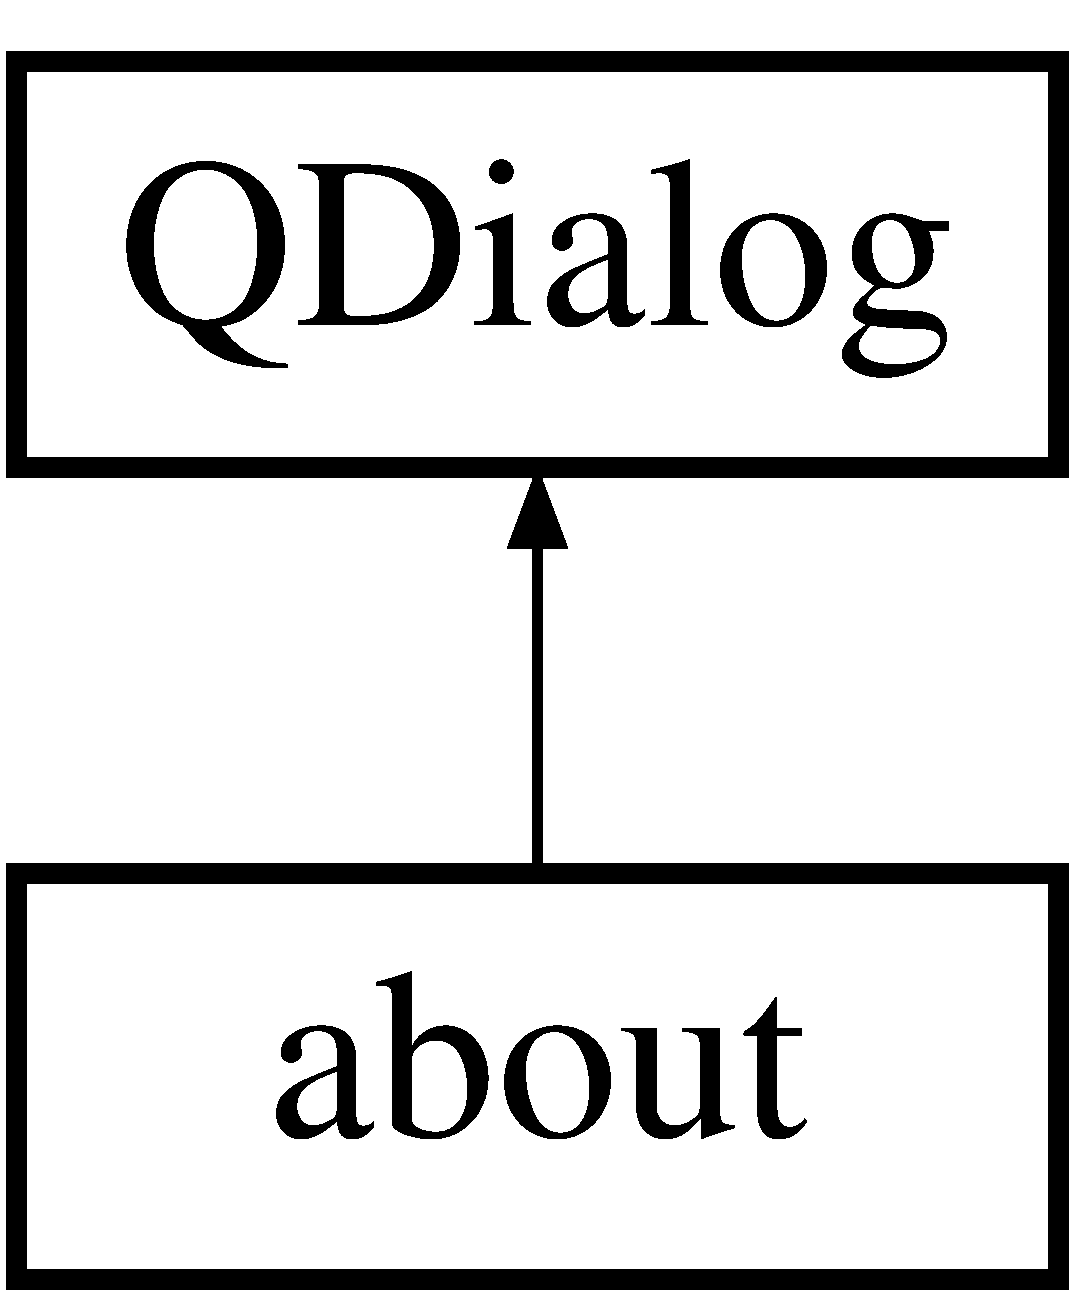
\includegraphics[height=2.000000cm]{classabout}
\end{center}
\end{figure}
\subsection*{Public Member Functions}
\begin{DoxyCompactItemize}
\item 
\hyperlink{classabout_ab16a8ec628d97aee17f0332e09964f52}{about} (Q\-Widget $\ast$parent=0)
\item 
\hyperlink{classabout_a0d7ebadcc35f58044fe6cbc7d8d4f636}{$\sim$about} ()
\end{DoxyCompactItemize}


\subsection{Detailed Description}
Contact class -\/ holds information for \char`\"{}\-About\char`\"{} dialog

\begin{DoxyAuthor}{Author}
richard (5/13/18) 
\end{DoxyAuthor}


\subsection{Constructor \& Destructor Documentation}
\hypertarget{classabout_ab16a8ec628d97aee17f0332e09964f52}{\index{about@{about}!about@{about}}
\index{about@{about}!about@{about}}
\subsubsection[{about}]{\setlength{\rightskip}{0pt plus 5cm}about\-::about (
\begin{DoxyParamCaption}
\item[{Q\-Widget $\ast$}]{parent = {\ttfamily 0}}
\end{DoxyParamCaption}
)\hspace{0.3cm}{\ttfamily [explicit]}}}\label{classabout_ab16a8ec628d97aee17f0332e09964f52}
about constructor -\/ requires a Qwidgit to draw on

\begin{DoxyAuthor}{Author}
richard (5/13/18)
\end{DoxyAuthor}

\begin{DoxyParams}{Parameters}
{\em parent} & \\
\hline
\end{DoxyParams}
\hypertarget{classabout_a0d7ebadcc35f58044fe6cbc7d8d4f636}{\index{about@{about}!$\sim$about@{$\sim$about}}
\index{$\sim$about@{$\sim$about}!about@{about}}
\subsubsection[{$\sim$about}]{\setlength{\rightskip}{0pt plus 5cm}about\-::$\sim$about (
\begin{DoxyParamCaption}
{}
\end{DoxyParamCaption}
)}}\label{classabout_a0d7ebadcc35f58044fe6cbc7d8d4f636}
about destructor -\/ release space

\begin{DoxyAuthor}{Author}
richard (5/13/18) 
\end{DoxyAuthor}


The documentation for this class was generated from the following files\-:\begin{DoxyCompactItemize}
\item 
/home/edt/\-C\-S1\-C/\-Class\-Project/\-Main\-Window/about.\-h\item 
/home/edt/\-C\-S1\-C/\-Class\-Project/\-Main\-Window/about.\-cpp\end{DoxyCompactItemize}

\hypertarget{classCircle}{\section{Circle Class Reference}
\label{classCircle}\index{Circle@{Circle}}
}


{\ttfamily \#include $<$circle.\-h$>$}

Inheritance diagram for Circle\-:\begin{figure}[H]
\begin{center}
\leavevmode
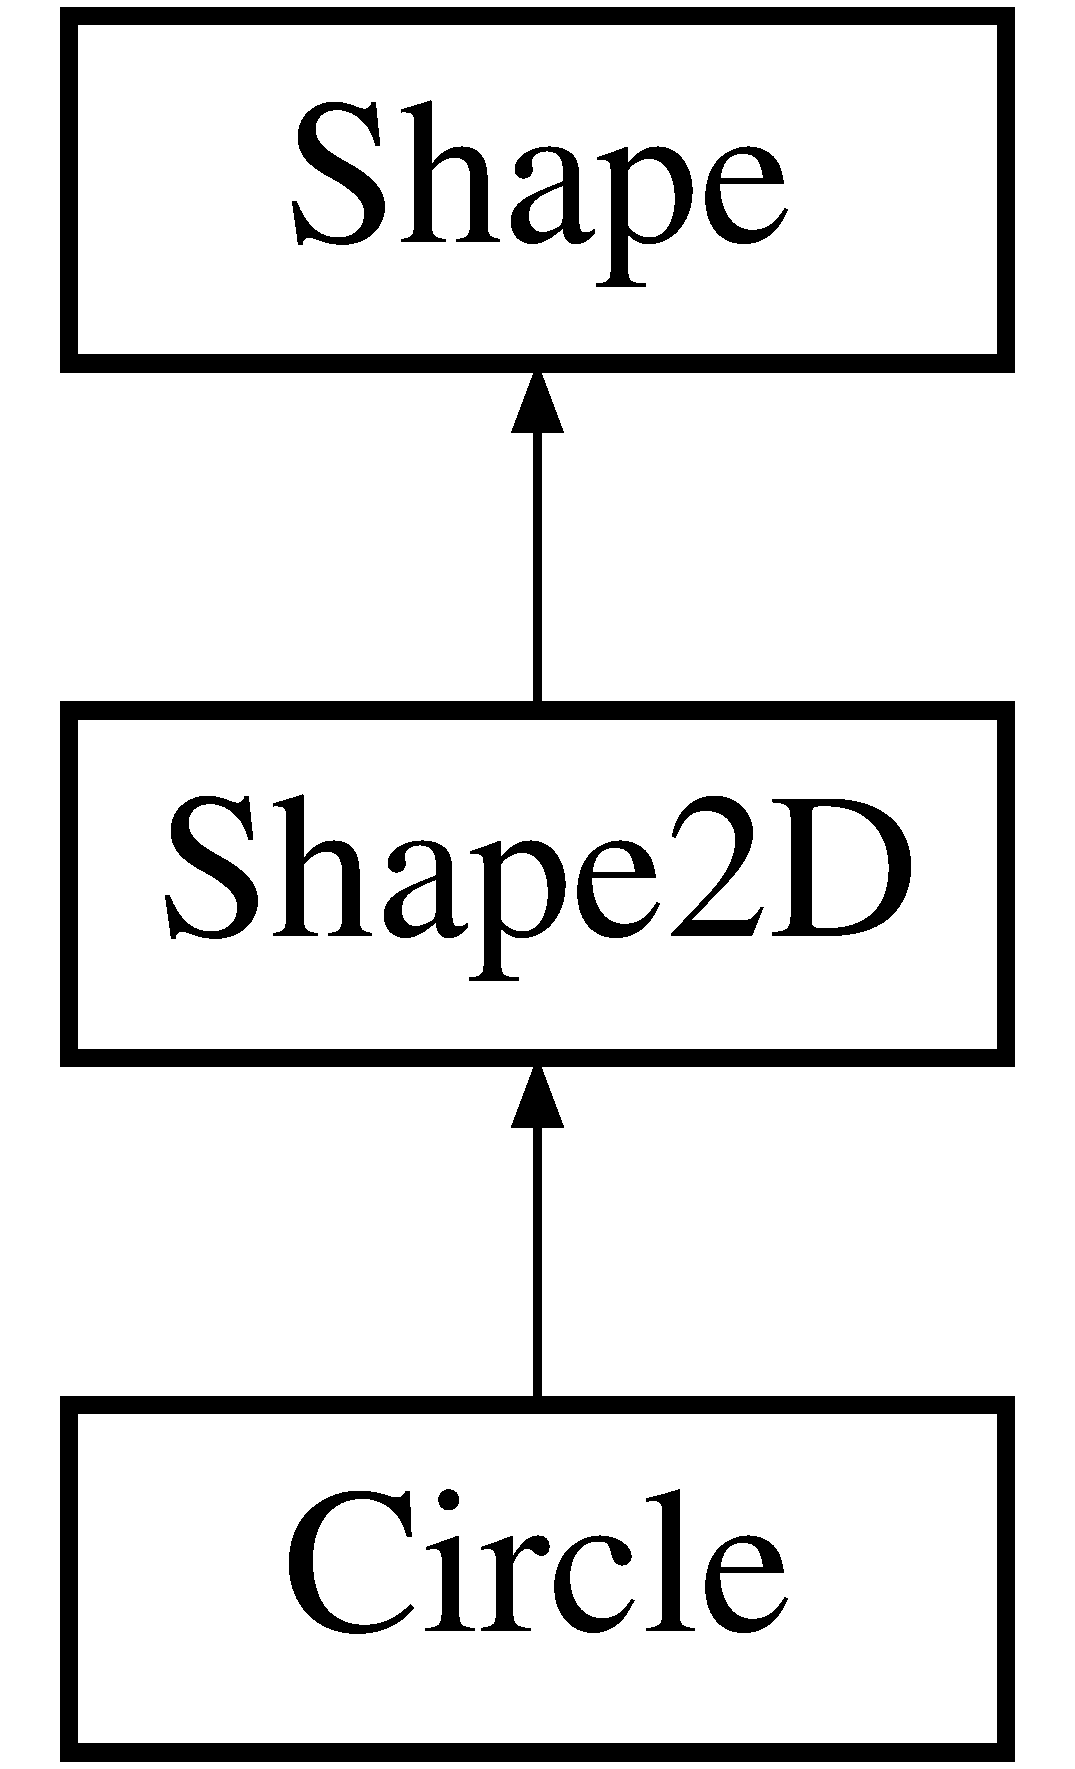
\includegraphics[height=3.000000cm]{classCircle}
\end{center}
\end{figure}
\subsection*{Public Member Functions}
\begin{DoxyCompactItemize}
\item 
\hyperlink{classCircle_af4337aa5f28b63e6e3f4fba0766e4b2f}{Circle} (Q\-Paint\-Device $\ast$device, int x\-Id, Q\-Color x\-Pen\-Color, qreal x\-Pen\-Width, Qt\-::\-Pen\-Style x\-Pen\-Style, Qt\-::\-Pen\-Cap\-Style x\-Pen\-Cap\-Style, Qt\-::\-Pen\-Join\-Style x\-Pen\-Join\-Style, Q\-Color x\-Brush\-Color, Qt\-::\-Brush\-Style x\-Brush\-Style, int x\-Top\-Left\-X, int x\-Top\-Left\-Y, int x\-Diameter)
\item 
\hypertarget{classCircle_a2067c595933e8313ea1baf8ee19545f4}{\hyperlink{classCircle}{Circle} \& {\bfseries operator=} (const \hyperlink{classCircle}{Circle} \&)=delete}\label{classCircle_a2067c595933e8313ea1baf8ee19545f4}

\item 
\hypertarget{classCircle_a36efc1546de87eef6ff11c61c0d4ff34}{{\bfseries Circle} (const \hyperlink{classCircle}{Circle} \&)=delete}\label{classCircle_a36efc1546de87eef6ff11c61c0d4ff34}

\item 
\hyperlink{classCircle_ae3f30436e645d73e368e8ee55f8d1650}{$\sim$\-Circle} ()
\item 
std\-::ostream \& \hyperlink{classCircle_a8afb61e2e5b24c95d0d4514da1d45bb2}{print} (std\-::ostream \&os) const 
\item 
void \hyperlink{classCircle_ae4d43ef78c3a06cb913bbd6a7dd94783}{draw} (Q\-Paint\-Device $\ast$device) override
\item 
void \hyperlink{classCircle_a48641bff5fb13da4bceb319862fd16c1}{move} (Q\-Point \&new\-Upper\-Left) override
\item 
void \hyperlink{classCircle_ae9c239fb51beadf9d6be4861473949f5}{update} (void) override
\item 
double \hyperlink{classCircle_ad6e363f95b6a42109527071724d8ea76}{calc\-Perimeter} () const override
\item 
double \hyperlink{classCircle_a2ebf184f1aed664e3858b65ce17fa798}{calc\-Area} () const override
\end{DoxyCompactItemize}
\subsection*{Additional Inherited Members}


\subsection{Detailed Description}
\hyperlink{classCircle}{Circle} class -\/ derived from \hyperlink{classShape2D}{Shape2\-D}

\begin{DoxyAuthor}{Author}
edt (5/13/18) 
\end{DoxyAuthor}


\subsection{Constructor \& Destructor Documentation}
\hypertarget{classCircle_af4337aa5f28b63e6e3f4fba0766e4b2f}{\index{Circle@{Circle}!Circle@{Circle}}
\index{Circle@{Circle}!Circle@{Circle}}
\subsubsection[{Circle}]{\setlength{\rightskip}{0pt plus 5cm}Circle\-::\-Circle (
\begin{DoxyParamCaption}
\item[{Q\-Paint\-Device $\ast$}]{device, }
\item[{int}]{x\-Id, }
\item[{Q\-Color}]{x\-Pen\-Color, }
\item[{qreal}]{x\-Pen\-Width, }
\item[{Qt\-::\-Pen\-Style}]{x\-Pen\-Style, }
\item[{Qt\-::\-Pen\-Cap\-Style}]{x\-Pen\-Cap\-Style, }
\item[{Qt\-::\-Pen\-Join\-Style}]{x\-Pen\-Join\-Style, }
\item[{Q\-Color}]{x\-Brush\-Color, }
\item[{Qt\-::\-Brush\-Style}]{x\-Brush\-Style, }
\item[{int}]{x\-Top\-Left\-X, }
\item[{int}]{x\-Top\-Left\-Y, }
\item[{int}]{x\-Diameter}
\end{DoxyParamCaption}
)}}\label{classCircle_af4337aa5f28b63e6e3f4fba0766e4b2f}
Constructor -\/ create a Q\-T drawable circle 2\-D

\begin{DoxyAuthor}{Author}
edt (5/13/18)
\end{DoxyAuthor}

\begin{DoxyParams}{Parameters}
{\em device} & -\/ Q\-Paint\-Device \\
\hline
{\em x\-Id} & -\/ shape I\-D \\
\hline
{\em x\-Pen\-Color} & \\
\hline
{\em x\-Pen\-Width} & \\
\hline
{\em x\-Pen\-Style} & \\
\hline
{\em x\-Pen\-Cap\-Style} & \\
\hline
{\em x\-Pen\-Join\-Style} & \\
\hline
{\em x\-Brush\-Color} & \\
\hline
{\em x\-Brush\-Style} & \\
\hline
{\em x\-Top\-Left\-X} & \\
\hline
{\em x\-Top\-Left\-Y} & \\
\hline
{\em x\-Diameter} & \\
\hline
\end{DoxyParams}
\hypertarget{classCircle_ae3f30436e645d73e368e8ee55f8d1650}{\index{Circle@{Circle}!$\sim$\-Circle@{$\sim$\-Circle}}
\index{$\sim$\-Circle@{$\sim$\-Circle}!Circle@{Circle}}
\subsubsection[{$\sim$\-Circle}]{\setlength{\rightskip}{0pt plus 5cm}Circle\-::$\sim$\-Circle (
\begin{DoxyParamCaption}
{}
\end{DoxyParamCaption}
)}}\label{classCircle_ae3f30436e645d73e368e8ee55f8d1650}
Destructor -\/ simply free the object space

\begin{DoxyAuthor}{Author}
edt (5/13/18) 
\end{DoxyAuthor}


\subsection{Member Function Documentation}
\hypertarget{classCircle_a2ebf184f1aed664e3858b65ce17fa798}{\index{Circle@{Circle}!calc\-Area@{calc\-Area}}
\index{calc\-Area@{calc\-Area}!Circle@{Circle}}
\subsubsection[{calc\-Area}]{\setlength{\rightskip}{0pt plus 5cm}double Circle\-::calc\-Area (
\begin{DoxyParamCaption}
\item[{void}]{}
\end{DoxyParamCaption}
) const\hspace{0.3cm}{\ttfamily [override]}, {\ttfamily [virtual]}}}\label{classCircle_a2ebf184f1aed664e3858b65ce17fa798}
calc\-Area -\/ determine area enclosed by object

\begin{DoxyAuthor}{Author}
edt (5/13/18)
\end{DoxyAuthor}
\begin{DoxyReturn}{Returns}
double 
\end{DoxyReturn}


Implements \hyperlink{classShape}{Shape}.

\hypertarget{classCircle_ad6e363f95b6a42109527071724d8ea76}{\index{Circle@{Circle}!calc\-Perimeter@{calc\-Perimeter}}
\index{calc\-Perimeter@{calc\-Perimeter}!Circle@{Circle}}
\subsubsection[{calc\-Perimeter}]{\setlength{\rightskip}{0pt plus 5cm}double Circle\-::calc\-Perimeter (
\begin{DoxyParamCaption}
\item[{void}]{}
\end{DoxyParamCaption}
) const\hspace{0.3cm}{\ttfamily [override]}, {\ttfamily [virtual]}}}\label{classCircle_ad6e363f95b6a42109527071724d8ea76}
calc\-Perimeter -\/ determine object outline length

\begin{DoxyAuthor}{Author}
edt (5/13/18)
\end{DoxyAuthor}
\begin{DoxyReturn}{Returns}
double 
\end{DoxyReturn}


Implements \hyperlink{classShape}{Shape}.

\hypertarget{classCircle_ae4d43ef78c3a06cb913bbd6a7dd94783}{\index{Circle@{Circle}!draw@{draw}}
\index{draw@{draw}!Circle@{Circle}}
\subsubsection[{draw}]{\setlength{\rightskip}{0pt plus 5cm}void Circle\-::draw (
\begin{DoxyParamCaption}
\item[{Q\-Paint\-Device $\ast$}]{device}
\end{DoxyParamCaption}
)\hspace{0.3cm}{\ttfamily [override]}, {\ttfamily [virtual]}}}\label{classCircle_ae4d43ef78c3a06cb913bbd6a7dd94783}
draw -\/ output object onto Q\-T canvas using Q\-Paint\-Device

\begin{DoxyAuthor}{Author}
edt (5/13/18)
\end{DoxyAuthor}

\begin{DoxyParams}{Parameters}
{\em device} & \\
\hline
\end{DoxyParams}


Implements \hyperlink{classShape}{Shape}.

\hypertarget{classCircle_a48641bff5fb13da4bceb319862fd16c1}{\index{Circle@{Circle}!move@{move}}
\index{move@{move}!Circle@{Circle}}
\subsubsection[{move}]{\setlength{\rightskip}{0pt plus 5cm}void Circle\-::move (
\begin{DoxyParamCaption}
\item[{Q\-Point \&}]{new\-Upper\-Left}
\end{DoxyParamCaption}
)\hspace{0.3cm}{\ttfamily [override]}, {\ttfamily [virtual]}}}\label{classCircle_a48641bff5fb13da4bceb319862fd16c1}
move -\/ relocate circle to new upper left coordinate

\begin{DoxyAuthor}{Author}
edt (5/13/18)
\end{DoxyAuthor}

\begin{DoxyParams}{Parameters}
{\em new\-Upper\-Left} & -\/ new location of upper left of enclosing rectangle \\
\hline
\end{DoxyParams}


Implements \hyperlink{classShape}{Shape}.

\hypertarget{classCircle_a8afb61e2e5b24c95d0d4514da1d45bb2}{\index{Circle@{Circle}!print@{print}}
\index{print@{print}!Circle@{Circle}}
\subsubsection[{print}]{\setlength{\rightskip}{0pt plus 5cm}std\-::ostream \& Circle\-::print (
\begin{DoxyParamCaption}
\item[{std\-::ostream \&}]{os}
\end{DoxyParamCaption}
) const\hspace{0.3cm}{\ttfamily [virtual]}}}\label{classCircle_a8afb61e2e5b24c95d0d4514da1d45bb2}
print -\/ print limited information about derived instance for debugging

\begin{DoxyAuthor}{Author}
edt (5/13/18)
\end{DoxyAuthor}

\begin{DoxyParams}{Parameters}
{\em os} & -\/ output stream\\
\hline
\end{DoxyParams}
\begin{DoxyReturn}{Returns}
std\-::ostream\& 
\end{DoxyReturn}


Implements \hyperlink{classShape2D_a6faf0b7950ea77a2ec6f29a31d65a624}{Shape2\-D}.

\hypertarget{classCircle_ae9c239fb51beadf9d6be4861473949f5}{\index{Circle@{Circle}!update@{update}}
\index{update@{update}!Circle@{Circle}}
\subsubsection[{update}]{\setlength{\rightskip}{0pt plus 5cm}void Circle\-::update (
\begin{DoxyParamCaption}
\item[{void}]{}
\end{DoxyParamCaption}
)\hspace{0.3cm}{\ttfamily [override]}, {\ttfamily [virtual]}}}\label{classCircle_ae9c239fb51beadf9d6be4861473949f5}
update -\/ force redraw of object

\begin{DoxyAuthor}{Author}
edt (5/13/18)
\end{DoxyAuthor}

\begin{DoxyParams}{Parameters}
{\em void} & \\
\hline
\end{DoxyParams}


Implements \hyperlink{classShape}{Shape}.



The documentation for this class was generated from the following files\-:\begin{DoxyCompactItemize}
\item 
/home/edt/\-C\-S1\-C/\-Class\-Project/\-Main\-Window/circle.\-h\item 
/home/edt/\-C\-S1\-C/\-Class\-Project/\-Main\-Window/circle.\-cpp\end{DoxyCompactItemize}

\hypertarget{structcompare__shape__area}{\section{compare\-\_\-shape\-\_\-area Struct Reference}
\label{structcompare__shape__area}\index{compare\-\_\-shape\-\_\-area@{compare\-\_\-shape\-\_\-area}}
}


{\ttfamily \#include $<$shape.\-h$>$}

\subsection*{Public Member Functions}
\begin{DoxyCompactItemize}
\item 
bool \hyperlink{structcompare__shape__area_a6cb9a97d4dfb63051ce4d1b8e96f7eb3}{operator()} (const \hyperlink{classShape}{Shape} $\ast$s1, const \hyperlink{classShape}{Shape} $\ast$s2) const 
\end{DoxyCompactItemize}


\subsection{Detailed Description}
\hyperlink{structcompare__shape__perimeter}{compare\-\_\-shape\-\_\-perimeter} -\/ function object to facilitate sorting by shape area

\begin{DoxyAuthor}{Author}
edt (5/14/18) 
\end{DoxyAuthor}


\subsection{Member Function Documentation}
\hypertarget{structcompare__shape__area_a6cb9a97d4dfb63051ce4d1b8e96f7eb3}{\index{compare\-\_\-shape\-\_\-area@{compare\-\_\-shape\-\_\-area}!operator()@{operator()}}
\index{operator()@{operator()}!compare_shape_area@{compare\-\_\-shape\-\_\-area}}
\subsubsection[{operator()}]{\setlength{\rightskip}{0pt plus 5cm}bool compare\-\_\-shape\-\_\-area\-::operator() (
\begin{DoxyParamCaption}
\item[{const {\bf Shape} $\ast$}]{s1, }
\item[{const {\bf Shape} $\ast$}]{s2}
\end{DoxyParamCaption}
) const\hspace{0.3cm}{\ttfamily [inline]}}}\label{structcompare__shape__area_a6cb9a97d4dfb63051ce4d1b8e96f7eb3}
operator() -\/ function to compare two shape areas

\begin{DoxyAuthor}{Author}
edt (5/14/18)
\end{DoxyAuthor}

\begin{DoxyParams}{Parameters}
{\em s1} & -\/ first shape to compare \\
\hline
{\em s2} & -\/ second shape to compare\\
\hline
\end{DoxyParams}
\begin{DoxyReturn}{Returns}
bool -\/ true if first \hyperlink{classShape}{Shape}'s area less than second \hyperlink{classShape}{Shape} 
\end{DoxyReturn}


The documentation for this struct was generated from the following file\-:\begin{DoxyCompactItemize}
\item 
/home/edt/\-C\-S1\-C/\-Class\-Project/\-Main\-Window/shape.\-h\end{DoxyCompactItemize}

\hypertarget{structcompare__shape__id}{\section{compare\-\_\-shape\-\_\-id Struct Reference}
\label{structcompare__shape__id}\index{compare\-\_\-shape\-\_\-id@{compare\-\_\-shape\-\_\-id}}
}


{\ttfamily \#include $<$shape.\-h$>$}

\subsection*{Public Member Functions}
\begin{DoxyCompactItemize}
\item 
bool \hyperlink{structcompare__shape__id_a9fbd60d5f10cdc03e464607b96180592}{operator()} (const \hyperlink{classShape}{Shape} $\ast$s1, const \hyperlink{classShape}{Shape} $\ast$s2) const 
\end{DoxyCompactItemize}


\subsection{Detailed Description}
\hyperlink{structcompare__shape__id}{compare\-\_\-shape\-\_\-id} -\/ function object to facilitate sorting by shape I\-D

\begin{DoxyAuthor}{Author}
edt (5/14/18) 
\end{DoxyAuthor}


\subsection{Member Function Documentation}
\hypertarget{structcompare__shape__id_a9fbd60d5f10cdc03e464607b96180592}{\index{compare\-\_\-shape\-\_\-id@{compare\-\_\-shape\-\_\-id}!operator()@{operator()}}
\index{operator()@{operator()}!compare_shape_id@{compare\-\_\-shape\-\_\-id}}
\subsubsection[{operator()}]{\setlength{\rightskip}{0pt plus 5cm}bool compare\-\_\-shape\-\_\-id\-::operator() (
\begin{DoxyParamCaption}
\item[{const {\bf Shape} $\ast$}]{s1, }
\item[{const {\bf Shape} $\ast$}]{s2}
\end{DoxyParamCaption}
) const\hspace{0.3cm}{\ttfamily [inline]}}}\label{structcompare__shape__id_a9fbd60d5f10cdc03e464607b96180592}
operator() -\/ function to compare two shape I\-Ds

\begin{DoxyAuthor}{Author}
edt (5/14/18)
\end{DoxyAuthor}

\begin{DoxyParams}{Parameters}
{\em s1} & -\/ first shape to compare \\
\hline
{\em s2} & -\/ second shape to compare\\
\hline
\end{DoxyParams}
\begin{DoxyReturn}{Returns}
bool -\/ true if first \hyperlink{classShape}{Shape}'s I\-D less than second \hyperlink{classShape}{Shape} 
\end{DoxyReturn}


The documentation for this struct was generated from the following file\-:\begin{DoxyCompactItemize}
\item 
/home/edt/\-C\-S1\-C/\-Class\-Project/\-Main\-Window/shape.\-h\end{DoxyCompactItemize}

\hypertarget{structcompare__shape__perimeter}{\section{compare\-\_\-shape\-\_\-perimeter Struct Reference}
\label{structcompare__shape__perimeter}\index{compare\-\_\-shape\-\_\-perimeter@{compare\-\_\-shape\-\_\-perimeter}}
}


{\ttfamily \#include $<$shape.\-h$>$}

\subsection*{Public Member Functions}
\begin{DoxyCompactItemize}
\item 
bool \hyperlink{structcompare__shape__perimeter_a534c21fb89ea2bcc5ecbc4b1d96b4110}{operator()} (const \hyperlink{classShape}{Shape} $\ast$s1, const \hyperlink{classShape}{Shape} $\ast$s2) const 
\end{DoxyCompactItemize}


\subsection{Detailed Description}
\hyperlink{structcompare__shape__perimeter}{compare\-\_\-shape\-\_\-perimeter} -\/ function object to facilitate sorting by shape perimeter

\begin{DoxyAuthor}{Author}
edt (5/14/18) 
\end{DoxyAuthor}


\subsection{Member Function Documentation}
\hypertarget{structcompare__shape__perimeter_a534c21fb89ea2bcc5ecbc4b1d96b4110}{\index{compare\-\_\-shape\-\_\-perimeter@{compare\-\_\-shape\-\_\-perimeter}!operator()@{operator()}}
\index{operator()@{operator()}!compare_shape_perimeter@{compare\-\_\-shape\-\_\-perimeter}}
\subsubsection[{operator()}]{\setlength{\rightskip}{0pt plus 5cm}bool compare\-\_\-shape\-\_\-perimeter\-::operator() (
\begin{DoxyParamCaption}
\item[{const {\bf Shape} $\ast$}]{s1, }
\item[{const {\bf Shape} $\ast$}]{s2}
\end{DoxyParamCaption}
) const\hspace{0.3cm}{\ttfamily [inline]}}}\label{structcompare__shape__perimeter_a534c21fb89ea2bcc5ecbc4b1d96b4110}
operator() -\/ function to compare two shape perimeters \begin{DoxyAuthor}{Author}
edt (5/14/18)
\end{DoxyAuthor}

\begin{DoxyParams}{Parameters}
{\em s1} & -\/ first shape to compare \\
\hline
{\em s2} & -\/ second shape to compare\\
\hline
\end{DoxyParams}
\begin{DoxyReturn}{Returns}
bool -\/ true if first \hyperlink{classShape}{Shape}'s perimeter less than second \hyperlink{classShape}{Shape} 
\end{DoxyReturn}


The documentation for this struct was generated from the following file\-:\begin{DoxyCompactItemize}
\item 
/home/edt/\-C\-S1\-C/\-Class\-Project/\-Main\-Window/shape.\-h\end{DoxyCompactItemize}

\hypertarget{classcontact}{\section{contact Class Reference}
\label{classcontact}\index{contact@{contact}}
}


{\ttfamily \#include $<$contact.\-h$>$}

Inheritance diagram for contact\-:\begin{figure}[H]
\begin{center}
\leavevmode
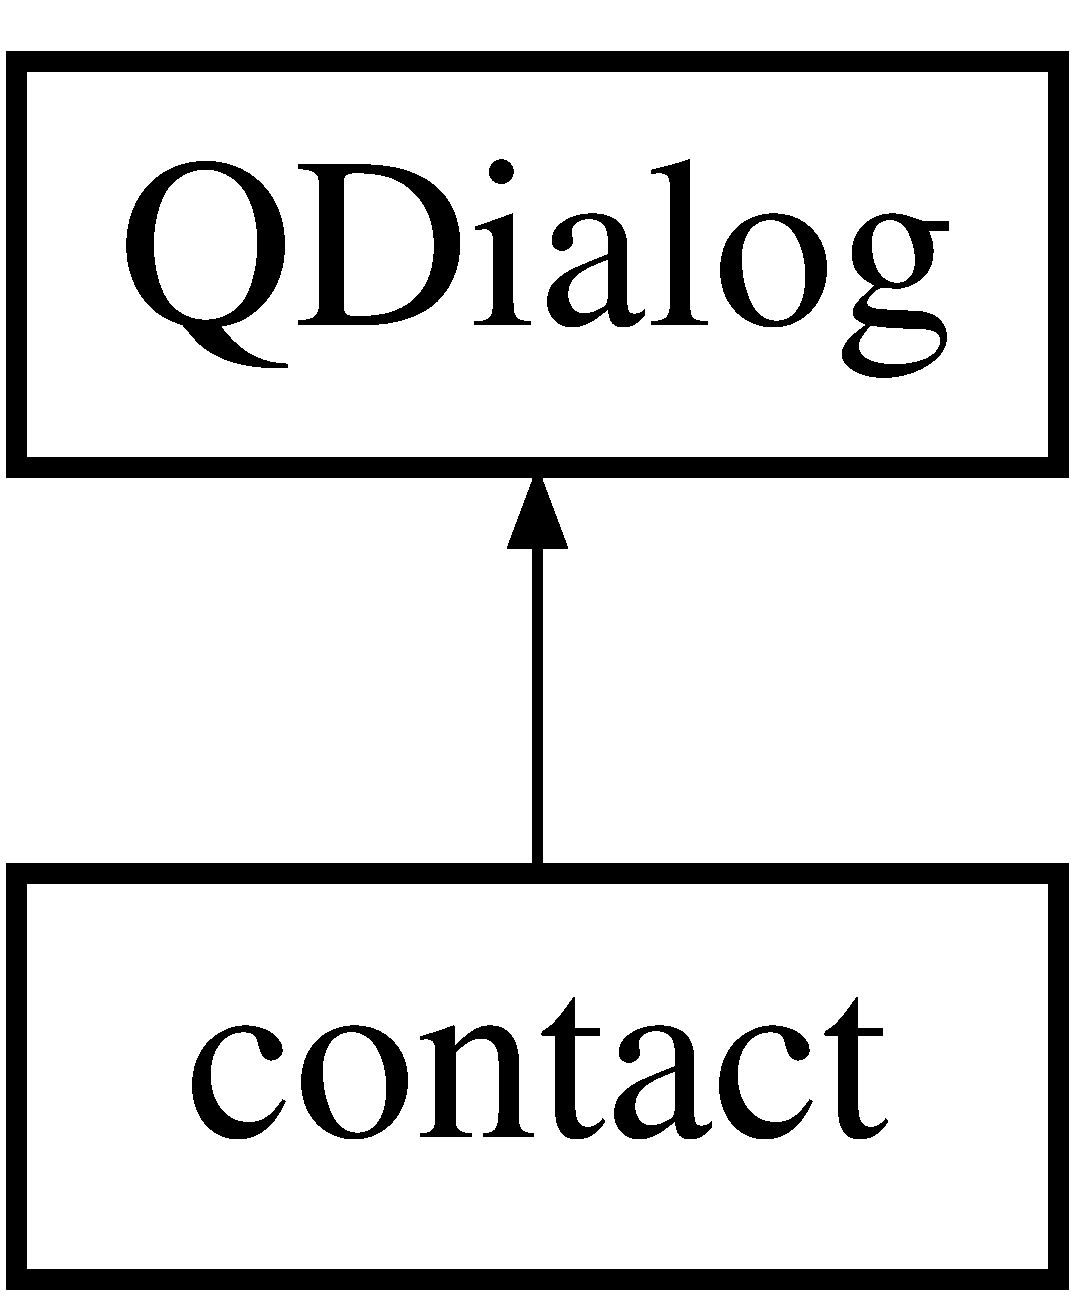
\includegraphics[height=2.000000cm]{classcontact}
\end{center}
\end{figure}
\subsection*{Public Member Functions}
\begin{DoxyCompactItemize}
\item 
\hyperlink{classcontact_a530a040af99efa8cb80a0e97fbd1bf34}{contact} (Q\-Widget $\ast$parent=0)
\item 
\hyperlink{classcontact_a326b92dd9a083dac47e636557d346195}{$\sim$contact} ()
\end{DoxyCompactItemize}


\subsection{Detailed Description}
Contact class -\/ holds information for \char`\"{}\-Contact Us\char`\"{} dialog

\begin{DoxyAuthor}{Author}
richard (5/13/18) 
\end{DoxyAuthor}


\subsection{Constructor \& Destructor Documentation}
\hypertarget{classcontact_a530a040af99efa8cb80a0e97fbd1bf34}{\index{contact@{contact}!contact@{contact}}
\index{contact@{contact}!contact@{contact}}
\subsubsection[{contact}]{\setlength{\rightskip}{0pt plus 5cm}contact\-::contact (
\begin{DoxyParamCaption}
\item[{Q\-Widget $\ast$}]{parent = {\ttfamily 0}}
\end{DoxyParamCaption}
)\hspace{0.3cm}{\ttfamily [explicit]}}}\label{classcontact_a530a040af99efa8cb80a0e97fbd1bf34}
contact constructor -\/ requires a Qwidgit to draw on

\begin{DoxyAuthor}{Author}
richard (5/13/18)
\end{DoxyAuthor}

\begin{DoxyParams}{Parameters}
{\em parent} & \\
\hline
\end{DoxyParams}
\hypertarget{classcontact_a326b92dd9a083dac47e636557d346195}{\index{contact@{contact}!$\sim$contact@{$\sim$contact}}
\index{$\sim$contact@{$\sim$contact}!contact@{contact}}
\subsubsection[{$\sim$contact}]{\setlength{\rightskip}{0pt plus 5cm}contact\-::$\sim$contact (
\begin{DoxyParamCaption}
{}
\end{DoxyParamCaption}
)}}\label{classcontact_a326b92dd9a083dac47e636557d346195}
contact destructor -\/ release space

\begin{DoxyAuthor}{Author}
richard (5/13/18) 
\end{DoxyAuthor}


The documentation for this class was generated from the following files\-:\begin{DoxyCompactItemize}
\item 
/home/edt/\-C\-S1\-C/\-Class\-Project/\-Main\-Window/contact.\-h\item 
/home/edt/\-C\-S1\-C/\-Class\-Project/\-Main\-Window/contact.\-cpp\end{DoxyCompactItemize}

\hypertarget{classEllipse}{\section{Ellipse Class Reference}
\label{classEllipse}\index{Ellipse@{Ellipse}}
}


{\ttfamily \#include $<$ellipse.\-h$>$}

Inheritance diagram for Ellipse\-:\begin{figure}[H]
\begin{center}
\leavevmode
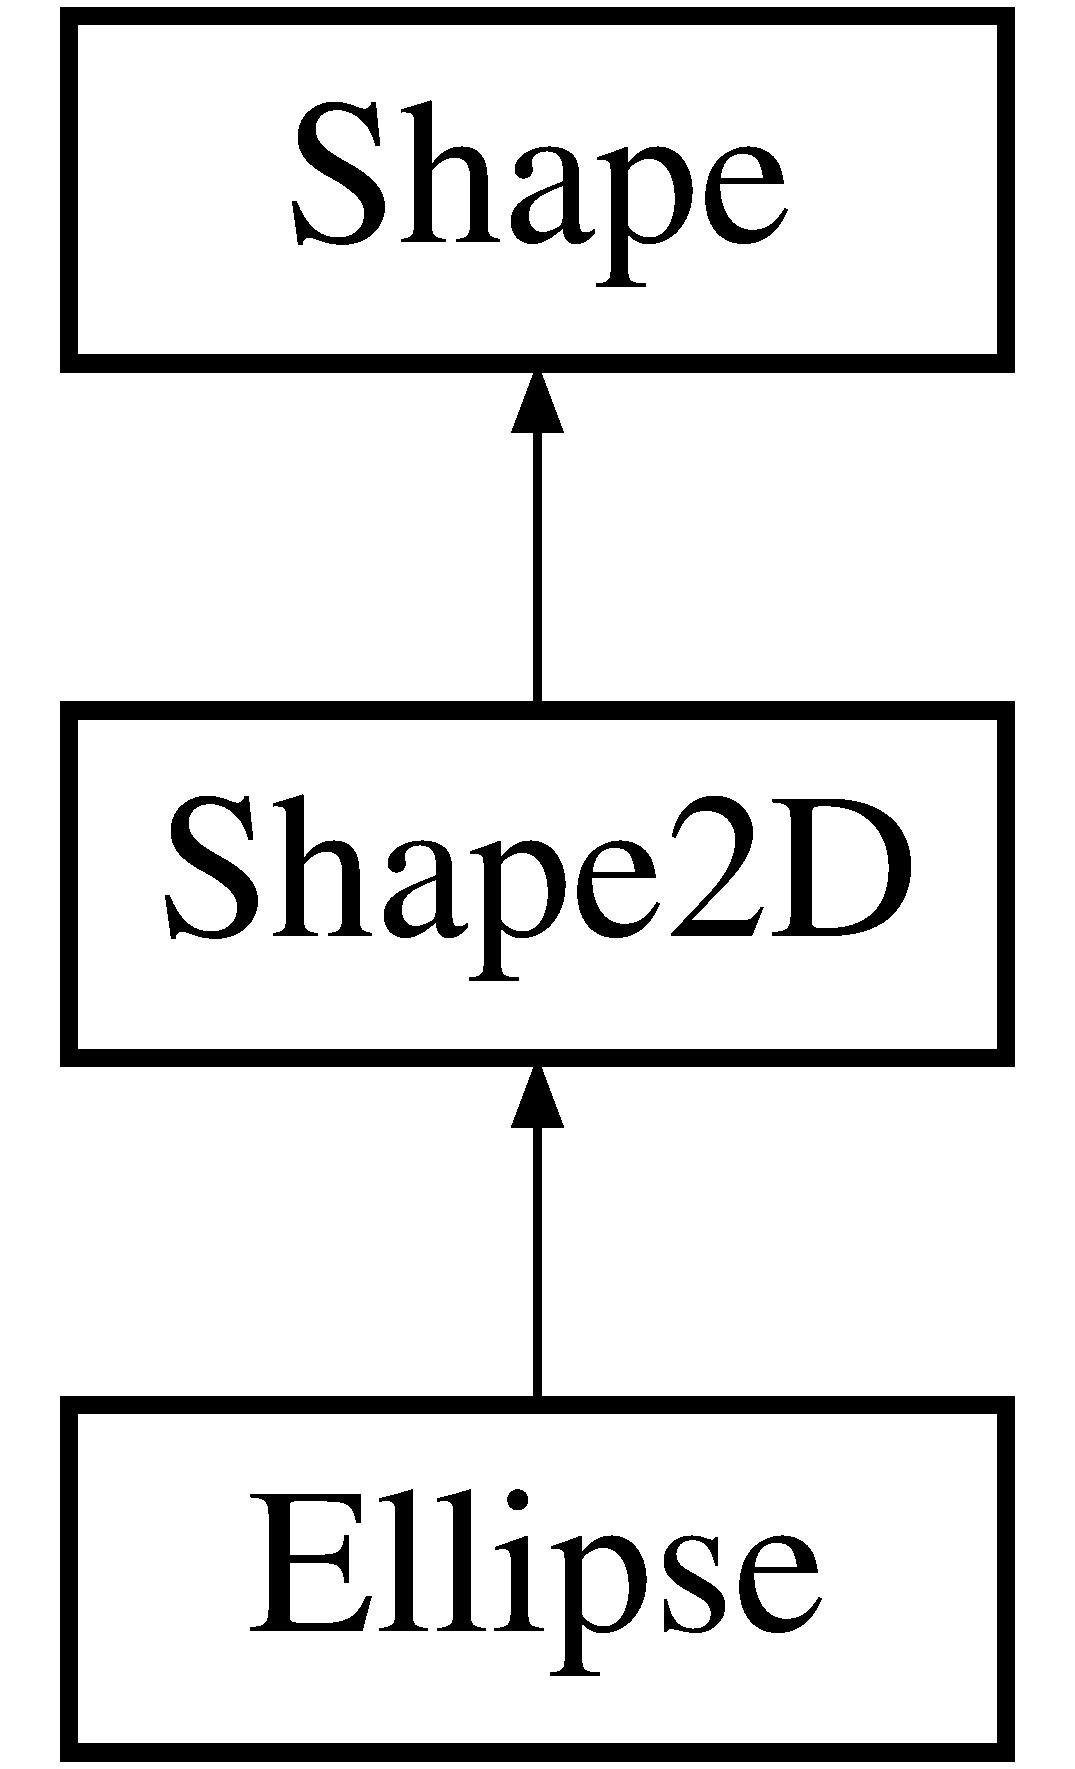
\includegraphics[height=3.000000cm]{classEllipse}
\end{center}
\end{figure}
\subsection*{Public Member Functions}
\begin{DoxyCompactItemize}
\item 
\hyperlink{classEllipse_acec99b1c3bac3534d5c1c9ded420e29f}{Ellipse} (Q\-Paint\-Device $\ast$device, int x\-Id, Q\-Color x\-Pen\-Color, qreal x\-Pen\-Width, Qt\-::\-Pen\-Style x\-Pen\-Style, Qt\-::\-Pen\-Cap\-Style x\-Pen\-Cap\-Style, Qt\-::\-Pen\-Join\-Style x\-Pen\-Join\-Style, Q\-Color x\-Brush\-Color, Qt\-::\-Brush\-Style x\-Brush\-Style, int x\-Top\-Left\-X, int x\-Top\-Left\-Y, int x\-Width, int x\-Height)
\item 
\hypertarget{classEllipse_ad9a01ff7963a3bb34becaa0849510f5f}{\hyperlink{classEllipse}{Ellipse} \& {\bfseries operator=} (const \hyperlink{classEllipse}{Ellipse} \&)=delete}\label{classEllipse_ad9a01ff7963a3bb34becaa0849510f5f}

\item 
\hypertarget{classEllipse_ae9069aaff10df80436665806fa3fd441}{{\bfseries Ellipse} (const \hyperlink{classEllipse}{Ellipse} \&)=delete}\label{classEllipse_ae9069aaff10df80436665806fa3fd441}

\item 
\hyperlink{classEllipse_a94271a8a2b16101a52491b7e81e28547}{$\sim$\-Ellipse} ()
\item 
std\-::ostream \& \hyperlink{classEllipse_a6cd8da652c6e66f465fb23253deab458}{print} (std\-::ostream \&os) const 
\item 
void \hyperlink{classEllipse_a15ee15d60a77d8b0bb1711d96b5dd062}{draw} (Q\-Paint\-Device $\ast$device)
\item 
void \hyperlink{classEllipse_a29e9857d31cd33aa127c7ab171575c88}{move} (Q\-Point \&new\-Upper\-Left)
\item 
void \hyperlink{classEllipse_a49d149cb6210f1b2fb58b10fbd8bed18}{update} (void)
\item 
double \hyperlink{classEllipse_a70f7a8edec42201d11c6fae43714c4c2}{calc\-Perimeter} () const 
\item 
double \hyperlink{classEllipse_a955141666e258fc582889a5f9298d798}{calc\-Area} () const 
\end{DoxyCompactItemize}
\subsection*{Additional Inherited Members}


\subsection{Detailed Description}
ellipse class derived from \hyperlink{classShape2D}{Shape2\-D}

\begin{DoxyAuthor}{Author}
edt (5/13/18) 
\end{DoxyAuthor}


\subsection{Constructor \& Destructor Documentation}
\hypertarget{classEllipse_acec99b1c3bac3534d5c1c9ded420e29f}{\index{Ellipse@{Ellipse}!Ellipse@{Ellipse}}
\index{Ellipse@{Ellipse}!Ellipse@{Ellipse}}
\subsubsection[{Ellipse}]{\setlength{\rightskip}{0pt plus 5cm}Ellipse\-::\-Ellipse (
\begin{DoxyParamCaption}
\item[{Q\-Paint\-Device $\ast$}]{device, }
\item[{int}]{x\-Id, }
\item[{Q\-Color}]{x\-Pen\-Color, }
\item[{qreal}]{x\-Pen\-Width, }
\item[{Qt\-::\-Pen\-Style}]{x\-Pen\-Style, }
\item[{Qt\-::\-Pen\-Cap\-Style}]{x\-Pen\-Cap\-Style, }
\item[{Qt\-::\-Pen\-Join\-Style}]{x\-Pen\-Join\-Style, }
\item[{Q\-Color}]{x\-Brush\-Color, }
\item[{Qt\-::\-Brush\-Style}]{x\-Brush\-Style, }
\item[{int}]{x\-Top\-Left\-X, }
\item[{int}]{x\-Top\-Left\-Y, }
\item[{int}]{x\-Width, }
\item[{int}]{x\-Height}
\end{DoxyParamCaption}
)}}\label{classEllipse_acec99b1c3bac3534d5c1c9ded420e29f}
ellipse constructor -\/ create Q\-T drawable object

\begin{DoxyAuthor}{Author}
edt (5/13/18)
\end{DoxyAuthor}

\begin{DoxyParams}{Parameters}
{\em device} & -\/ Q\-Paint\-Device \\
\hline
{\em x\-Id} & -\/ shape I\-D \\
\hline
{\em x\-Pen\-Color} & \\
\hline
{\em x\-Pen\-Width} & \\
\hline
{\em x\-Pen\-Style} & \\
\hline
{\em x\-Pen\-Cap\-Style} & \\
\hline
{\em x\-Pen\-Join\-Style} & \\
\hline
{\em x\-Brush\-Color} & \\
\hline
{\em x\-Brush\-Style} & \\
\hline
{\em x\-Top\-Left\-X} & \\
\hline
{\em x\-Top\-Left\-Y} & \\
\hline
{\em x\-Width} & \\
\hline
{\em x\-Height} & \\
\hline
\end{DoxyParams}
\hypertarget{classEllipse_a94271a8a2b16101a52491b7e81e28547}{\index{Ellipse@{Ellipse}!$\sim$\-Ellipse@{$\sim$\-Ellipse}}
\index{$\sim$\-Ellipse@{$\sim$\-Ellipse}!Ellipse@{Ellipse}}
\subsubsection[{$\sim$\-Ellipse}]{\setlength{\rightskip}{0pt plus 5cm}Ellipse\-::$\sim$\-Ellipse (
\begin{DoxyParamCaption}
{}
\end{DoxyParamCaption}
)}}\label{classEllipse_a94271a8a2b16101a52491b7e81e28547}
Destructor -\/ simply free the object space

\begin{DoxyAuthor}{Author}
edt (5/13/18) 
\end{DoxyAuthor}


\subsection{Member Function Documentation}
\hypertarget{classEllipse_a955141666e258fc582889a5f9298d798}{\index{Ellipse@{Ellipse}!calc\-Area@{calc\-Area}}
\index{calc\-Area@{calc\-Area}!Ellipse@{Ellipse}}
\subsubsection[{calc\-Area}]{\setlength{\rightskip}{0pt plus 5cm}double Ellipse\-::calc\-Area (
\begin{DoxyParamCaption}
\item[{void}]{}
\end{DoxyParamCaption}
) const\hspace{0.3cm}{\ttfamily [virtual]}}}\label{classEllipse_a955141666e258fc582889a5f9298d798}
calc\-Area -\/ determine area enclosed by object

\begin{DoxyAuthor}{Author}
edt (5/13/18)
\end{DoxyAuthor}
\begin{DoxyReturn}{Returns}
double 
\end{DoxyReturn}


Implements \hyperlink{classShape}{Shape}.

\hypertarget{classEllipse_a70f7a8edec42201d11c6fae43714c4c2}{\index{Ellipse@{Ellipse}!calc\-Perimeter@{calc\-Perimeter}}
\index{calc\-Perimeter@{calc\-Perimeter}!Ellipse@{Ellipse}}
\subsubsection[{calc\-Perimeter}]{\setlength{\rightskip}{0pt plus 5cm}double Ellipse\-::calc\-Perimeter (
\begin{DoxyParamCaption}
\item[{void}]{}
\end{DoxyParamCaption}
) const\hspace{0.3cm}{\ttfamily [virtual]}}}\label{classEllipse_a70f7a8edec42201d11c6fae43714c4c2}
calc\-Perimeter -\/ determine object outline length using Ramanujan Forumla \#1

\begin{DoxyAuthor}{Author}
edt (5/13/18)
\end{DoxyAuthor}
\begin{DoxyReturn}{Returns}
double 
\end{DoxyReturn}


Implements \hyperlink{classShape}{Shape}.

\hypertarget{classEllipse_a15ee15d60a77d8b0bb1711d96b5dd062}{\index{Ellipse@{Ellipse}!draw@{draw}}
\index{draw@{draw}!Ellipse@{Ellipse}}
\subsubsection[{draw}]{\setlength{\rightskip}{0pt plus 5cm}void Ellipse\-::draw (
\begin{DoxyParamCaption}
\item[{Q\-Paint\-Device $\ast$}]{device}
\end{DoxyParamCaption}
)\hspace{0.3cm}{\ttfamily [virtual]}}}\label{classEllipse_a15ee15d60a77d8b0bb1711d96b5dd062}
draw -\/ output object onto Q\-T canvas using Q\-Paint\-Device

\begin{DoxyAuthor}{Author}
edt (5/13/18)
\end{DoxyAuthor}

\begin{DoxyParams}{Parameters}
{\em device} & \\
\hline
\end{DoxyParams}


Implements \hyperlink{classShape}{Shape}.

\hypertarget{classEllipse_a29e9857d31cd33aa127c7ab171575c88}{\index{Ellipse@{Ellipse}!move@{move}}
\index{move@{move}!Ellipse@{Ellipse}}
\subsubsection[{move}]{\setlength{\rightskip}{0pt plus 5cm}void Ellipse\-::move (
\begin{DoxyParamCaption}
\item[{Q\-Point \&}]{new\-Upper\-Left}
\end{DoxyParamCaption}
)\hspace{0.3cm}{\ttfamily [virtual]}}}\label{classEllipse_a29e9857d31cd33aa127c7ab171575c88}
move -\/ relocate circle to new upper left coordinate

\begin{DoxyAuthor}{Author}
edt (5/13/18)
\end{DoxyAuthor}

\begin{DoxyParams}{Parameters}
{\em new\-Upper\-Left} & -\/ new location of upper left of enclosing rectangle \\
\hline
\end{DoxyParams}


Implements \hyperlink{classShape}{Shape}.

\hypertarget{classEllipse_a6cd8da652c6e66f465fb23253deab458}{\index{Ellipse@{Ellipse}!print@{print}}
\index{print@{print}!Ellipse@{Ellipse}}
\subsubsection[{print}]{\setlength{\rightskip}{0pt plus 5cm}std\-::ostream \& Ellipse\-::print (
\begin{DoxyParamCaption}
\item[{std\-::ostream \&}]{os}
\end{DoxyParamCaption}
) const\hspace{0.3cm}{\ttfamily [virtual]}}}\label{classEllipse_a6cd8da652c6e66f465fb23253deab458}
print -\/ print limited information about derived instance for debugging

\begin{DoxyAuthor}{Author}
edt (5/13/18)
\end{DoxyAuthor}

\begin{DoxyParams}{Parameters}
{\em os} & -\/ output stream pointer\\
\hline
\end{DoxyParams}
\begin{DoxyReturn}{Returns}
std\-::ostream\& 
\end{DoxyReturn}


Implements \hyperlink{classShape2D_a6faf0b7950ea77a2ec6f29a31d65a624}{Shape2\-D}.

\hypertarget{classEllipse_a49d149cb6210f1b2fb58b10fbd8bed18}{\index{Ellipse@{Ellipse}!update@{update}}
\index{update@{update}!Ellipse@{Ellipse}}
\subsubsection[{update}]{\setlength{\rightskip}{0pt plus 5cm}void Ellipse\-::update (
\begin{DoxyParamCaption}
\item[{void}]{}
\end{DoxyParamCaption}
)\hspace{0.3cm}{\ttfamily [virtual]}}}\label{classEllipse_a49d149cb6210f1b2fb58b10fbd8bed18}
update -\/ force redraw of object

\begin{DoxyAuthor}{Author}
edt (5/13/18)
\end{DoxyAuthor}

\begin{DoxyParams}{Parameters}
{\em void} & \\
\hline
\end{DoxyParams}


Implements \hyperlink{classShape}{Shape}.



The documentation for this class was generated from the following files\-:\begin{DoxyCompactItemize}
\item 
/home/edt/\-C\-S1\-C/\-Class\-Project/\-Main\-Window/ellipse.\-h\item 
/home/edt/\-C\-S1\-C/\-Class\-Project/\-Main\-Window/ellipse.\-cpp\end{DoxyCompactItemize}

\hypertarget{classLine}{\section{Line Class Reference}
\label{classLine}\index{Line@{Line}}
}


{\ttfamily \#include $<$line.\-h$>$}

Inheritance diagram for Line\-:\begin{figure}[H]
\begin{center}
\leavevmode
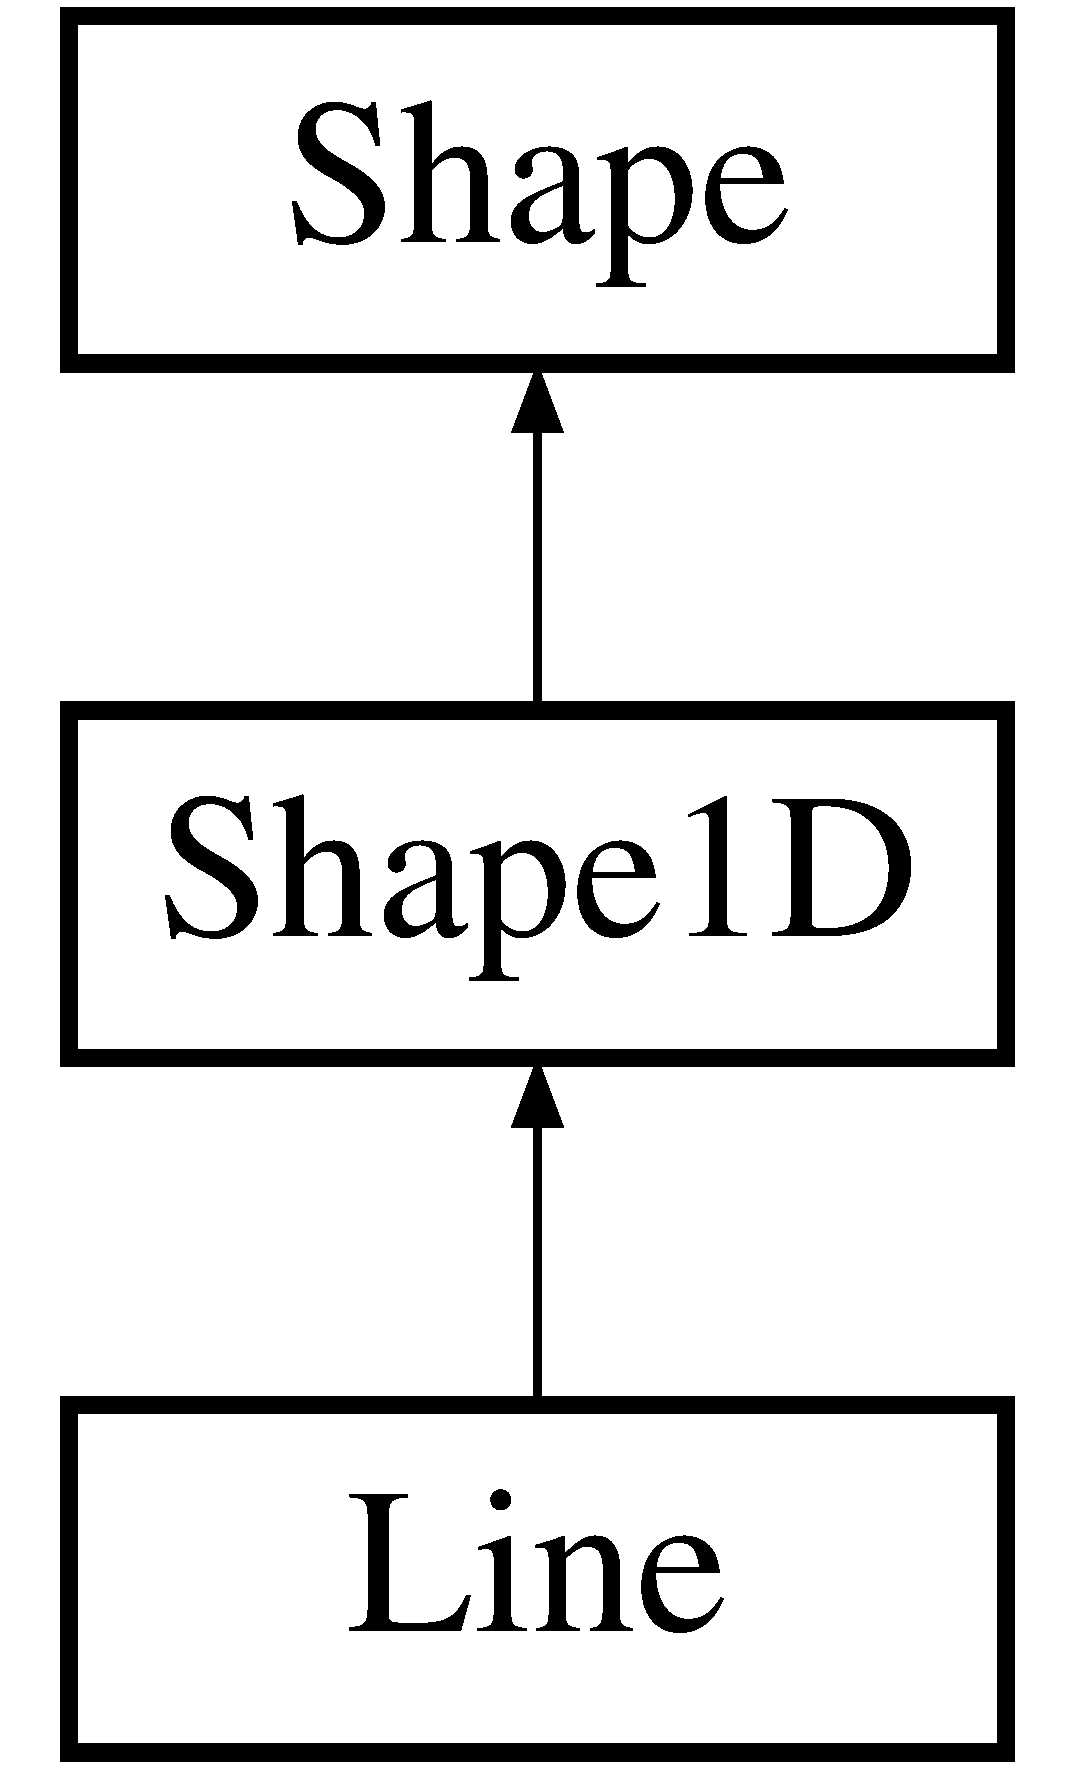
\includegraphics[height=3.000000cm]{classLine}
\end{center}
\end{figure}
\subsection*{Public Member Functions}
\begin{DoxyCompactItemize}
\item 
\hyperlink{classLine_a93d8a59e89500066516ca68a77a33d48}{Line} (Q\-Paint\-Device $\ast$device, int x\-Id, Q\-Color x\-Pen\-Color, qreal x\-Pen\-Width, Qt\-::\-Pen\-Style x\-Pen\-Style, Qt\-::\-Pen\-Cap\-Style x\-Pen\-Cap\-Style, Qt\-::\-Pen\-Join\-Style x\-Pen\-Join\-Style, int x\-Top\-Left\-X, int x\-Top\-Left\-Y, int x\-Bot\-Right\-X, int x\-Bot\-Right\-Y)
\item 
\hypertarget{classLine_a870c3c74ac53e7ce16586345b2181ad7}{\hyperlink{classLine}{Line} \& {\bfseries operator=} (const \hyperlink{classLine}{Line} \&)=delete}\label{classLine_a870c3c74ac53e7ce16586345b2181ad7}

\item 
\hypertarget{classLine_a39f1d91cfb4c01a8580d149af73c89b2}{{\bfseries Line} (const \hyperlink{classLine}{Line} \&)=delete}\label{classLine_a39f1d91cfb4c01a8580d149af73c89b2}

\item 
\hyperlink{classLine_aabe85f48d22d92b62257091f48174fac}{$\sim$\-Line} ()
\item 
std\-::ostream \& \hyperlink{classLine_a9535dc5fe2c3e66e548add6622e4b0ea}{print} (std\-::ostream \&os) const 
\item 
void \hyperlink{classLine_a5bb42c21fb963bbdca7c928f055376d5}{draw} (Q\-Paint\-Device $\ast$device)
\item 
void \hyperlink{classLine_acb2ae2fa8e058adbeea14c3966199090}{move} (Q\-Point \&new\-Upper\-Left)
\item 
void \hyperlink{classLine_a2338aa100616356ad580303478c102c2}{update} (void)
\item 
double \hyperlink{classLine_a804e2a31c02b0b5cfefe2e063e7fc52f}{calc\-Perimeter} () const 
\item 
double \hyperlink{classLine_ad4ab9f8147bd69fe385fcf5c14c5f46e}{calc\-Area} () const 
\end{DoxyCompactItemize}
\subsection*{Additional Inherited Members}


\subsection{Detailed Description}
\hyperlink{classLine}{Line} class -\/ derived from shape1\-D

\begin{DoxyAuthor}{Author}
edt (5/13/18) 
\end{DoxyAuthor}


\subsection{Constructor \& Destructor Documentation}
\hypertarget{classLine_a93d8a59e89500066516ca68a77a33d48}{\index{Line@{Line}!Line@{Line}}
\index{Line@{Line}!Line@{Line}}
\subsubsection[{Line}]{\setlength{\rightskip}{0pt plus 5cm}Line\-::\-Line (
\begin{DoxyParamCaption}
\item[{Q\-Paint\-Device $\ast$}]{device, }
\item[{int}]{x\-Id, }
\item[{Q\-Color}]{x\-Pen\-Color, }
\item[{qreal}]{x\-Pen\-Width, }
\item[{Qt\-::\-Pen\-Style}]{x\-Pen\-Style, }
\item[{Qt\-::\-Pen\-Cap\-Style}]{x\-Pen\-Cap\-Style, }
\item[{Qt\-::\-Pen\-Join\-Style}]{x\-Pen\-Join\-Style, }
\item[{int}]{x\-Top\-Left\-X, }
\item[{int}]{x\-Top\-Left\-Y, }
\item[{int}]{x\-Bot\-Right\-X, }
\item[{int}]{x\-Bot\-Right\-Y}
\end{DoxyParamCaption}
)}}\label{classLine_a93d8a59e89500066516ca68a77a33d48}
line constructor -\/ create Q\-T drawable object

\begin{DoxyAuthor}{Author}
edt (5/13/18)
\end{DoxyAuthor}

\begin{DoxyParams}{Parameters}
{\em device} & -\/ Q\-Paint\-Device \\
\hline
{\em x\-Id} & -\/ shape I\-D \\
\hline
{\em x\-Pen\-Color} & \\
\hline
{\em x\-Pen\-Width} & \\
\hline
{\em x\-Pen\-Style} & \\
\hline
{\em x\-Pen\-Cap\-Style} & \\
\hline
{\em x\-Pen\-Join\-Style} & \\
\hline
{\em x\-Top\-Left\-X} & \\
\hline
{\em x\-Top\-Left\-Y} & \\
\hline
{\em x\-Bot\-Right\-X} & \\
\hline
{\em x\-Bot\-Right\-Y} & \\
\hline
\end{DoxyParams}
\hypertarget{classLine_aabe85f48d22d92b62257091f48174fac}{\index{Line@{Line}!$\sim$\-Line@{$\sim$\-Line}}
\index{$\sim$\-Line@{$\sim$\-Line}!Line@{Line}}
\subsubsection[{$\sim$\-Line}]{\setlength{\rightskip}{0pt plus 5cm}Line\-::$\sim$\-Line (
\begin{DoxyParamCaption}
{}
\end{DoxyParamCaption}
)}}\label{classLine_aabe85f48d22d92b62257091f48174fac}
Destructor -\/ simply free the object space

\begin{DoxyAuthor}{Author}
edt (5/13/18) 
\end{DoxyAuthor}


\subsection{Member Function Documentation}
\hypertarget{classLine_ad4ab9f8147bd69fe385fcf5c14c5f46e}{\index{Line@{Line}!calc\-Area@{calc\-Area}}
\index{calc\-Area@{calc\-Area}!Line@{Line}}
\subsubsection[{calc\-Area}]{\setlength{\rightskip}{0pt plus 5cm}double Line\-::calc\-Area (
\begin{DoxyParamCaption}
\item[{void}]{}
\end{DoxyParamCaption}
) const\hspace{0.3cm}{\ttfamily [virtual]}}}\label{classLine_ad4ab9f8147bd69fe385fcf5c14c5f46e}
calc\-Area -\/ determine area enclosed by object

\begin{DoxyAuthor}{Author}
edt (5/13/18)
\end{DoxyAuthor}
\begin{DoxyReturn}{Returns}
double 
\end{DoxyReturn}


Implements \hyperlink{classShape}{Shape}.

\hypertarget{classLine_a804e2a31c02b0b5cfefe2e063e7fc52f}{\index{Line@{Line}!calc\-Perimeter@{calc\-Perimeter}}
\index{calc\-Perimeter@{calc\-Perimeter}!Line@{Line}}
\subsubsection[{calc\-Perimeter}]{\setlength{\rightskip}{0pt plus 5cm}double Line\-::calc\-Perimeter (
\begin{DoxyParamCaption}
\item[{void}]{}
\end{DoxyParamCaption}
) const\hspace{0.3cm}{\ttfamily [virtual]}}}\label{classLine_a804e2a31c02b0b5cfefe2e063e7fc52f}
calc\-Perimeter -\/ determine object outline length

\begin{DoxyAuthor}{Author}
edt (5/13/18)
\end{DoxyAuthor}
\begin{DoxyReturn}{Returns}
double 
\end{DoxyReturn}


Implements \hyperlink{classShape}{Shape}.

\hypertarget{classLine_a5bb42c21fb963bbdca7c928f055376d5}{\index{Line@{Line}!draw@{draw}}
\index{draw@{draw}!Line@{Line}}
\subsubsection[{draw}]{\setlength{\rightskip}{0pt plus 5cm}void Line\-::draw (
\begin{DoxyParamCaption}
\item[{Q\-Paint\-Device $\ast$}]{device}
\end{DoxyParamCaption}
)\hspace{0.3cm}{\ttfamily [virtual]}}}\label{classLine_a5bb42c21fb963bbdca7c928f055376d5}
draw -\/ output object onto Q\-T canvas using Q\-Paint\-Device

\begin{DoxyAuthor}{Author}
edt (5/13/18)
\end{DoxyAuthor}

\begin{DoxyParams}{Parameters}
{\em device} & \\
\hline
\end{DoxyParams}


Implements \hyperlink{classShape}{Shape}.

\hypertarget{classLine_acb2ae2fa8e058adbeea14c3966199090}{\index{Line@{Line}!move@{move}}
\index{move@{move}!Line@{Line}}
\subsubsection[{move}]{\setlength{\rightskip}{0pt plus 5cm}void Line\-::move (
\begin{DoxyParamCaption}
\item[{Q\-Point \&}]{new\-Upper\-Left}
\end{DoxyParamCaption}
)\hspace{0.3cm}{\ttfamily [virtual]}}}\label{classLine_acb2ae2fa8e058adbeea14c3966199090}
move -\/ relocate circle to new upper left coordinate

\begin{DoxyAuthor}{Author}
edt (5/13/18)
\end{DoxyAuthor}

\begin{DoxyParams}{Parameters}
{\em new\-Upper\-Left} & -\/ new location of upper left of enclosing rectangle \\
\hline
\end{DoxyParams}


Implements \hyperlink{classShape}{Shape}.

\hypertarget{classLine_a9535dc5fe2c3e66e548add6622e4b0ea}{\index{Line@{Line}!print@{print}}
\index{print@{print}!Line@{Line}}
\subsubsection[{print}]{\setlength{\rightskip}{0pt plus 5cm}std\-::ostream \& Line\-::print (
\begin{DoxyParamCaption}
\item[{std\-::ostream \&}]{os}
\end{DoxyParamCaption}
) const\hspace{0.3cm}{\ttfamily [virtual]}}}\label{classLine_a9535dc5fe2c3e66e548add6622e4b0ea}
print -\/ print limited information about derived instance for debugging

\begin{DoxyAuthor}{Author}
edt (5/13/18)
\end{DoxyAuthor}

\begin{DoxyParams}{Parameters}
{\em os} & -\/ output stream pointer\\
\hline
\end{DoxyParams}
\begin{DoxyReturn}{Returns}
std\-::ostream\& 
\end{DoxyReturn}


Implements \hyperlink{classShape1D_a20b9358df369b7b0fc4a1cdae5070836}{Shape1\-D}.

\hypertarget{classLine_a2338aa100616356ad580303478c102c2}{\index{Line@{Line}!update@{update}}
\index{update@{update}!Line@{Line}}
\subsubsection[{update}]{\setlength{\rightskip}{0pt plus 5cm}void Line\-::update (
\begin{DoxyParamCaption}
\item[{void}]{}
\end{DoxyParamCaption}
)\hspace{0.3cm}{\ttfamily [virtual]}}}\label{classLine_a2338aa100616356ad580303478c102c2}
update -\/ force redraw of object

\begin{DoxyAuthor}{Author}
edt (5/13/18)
\end{DoxyAuthor}

\begin{DoxyParams}{Parameters}
{\em void} & \\
\hline
\end{DoxyParams}


Implements \hyperlink{classShape}{Shape}.



The documentation for this class was generated from the following files\-:\begin{DoxyCompactItemize}
\item 
/home/edt/\-C\-S1\-C/\-Class\-Project/\-Main\-Window/line.\-h\item 
/home/edt/\-C\-S1\-C/\-Class\-Project/\-Main\-Window/line.\-cpp\end{DoxyCompactItemize}

\hypertarget{classlogin}{\section{login Class Reference}
\label{classlogin}\index{login@{login}}
}


{\ttfamily \#include $<$login.\-h$>$}

Inheritance diagram for login\-:\begin{figure}[H]
\begin{center}
\leavevmode
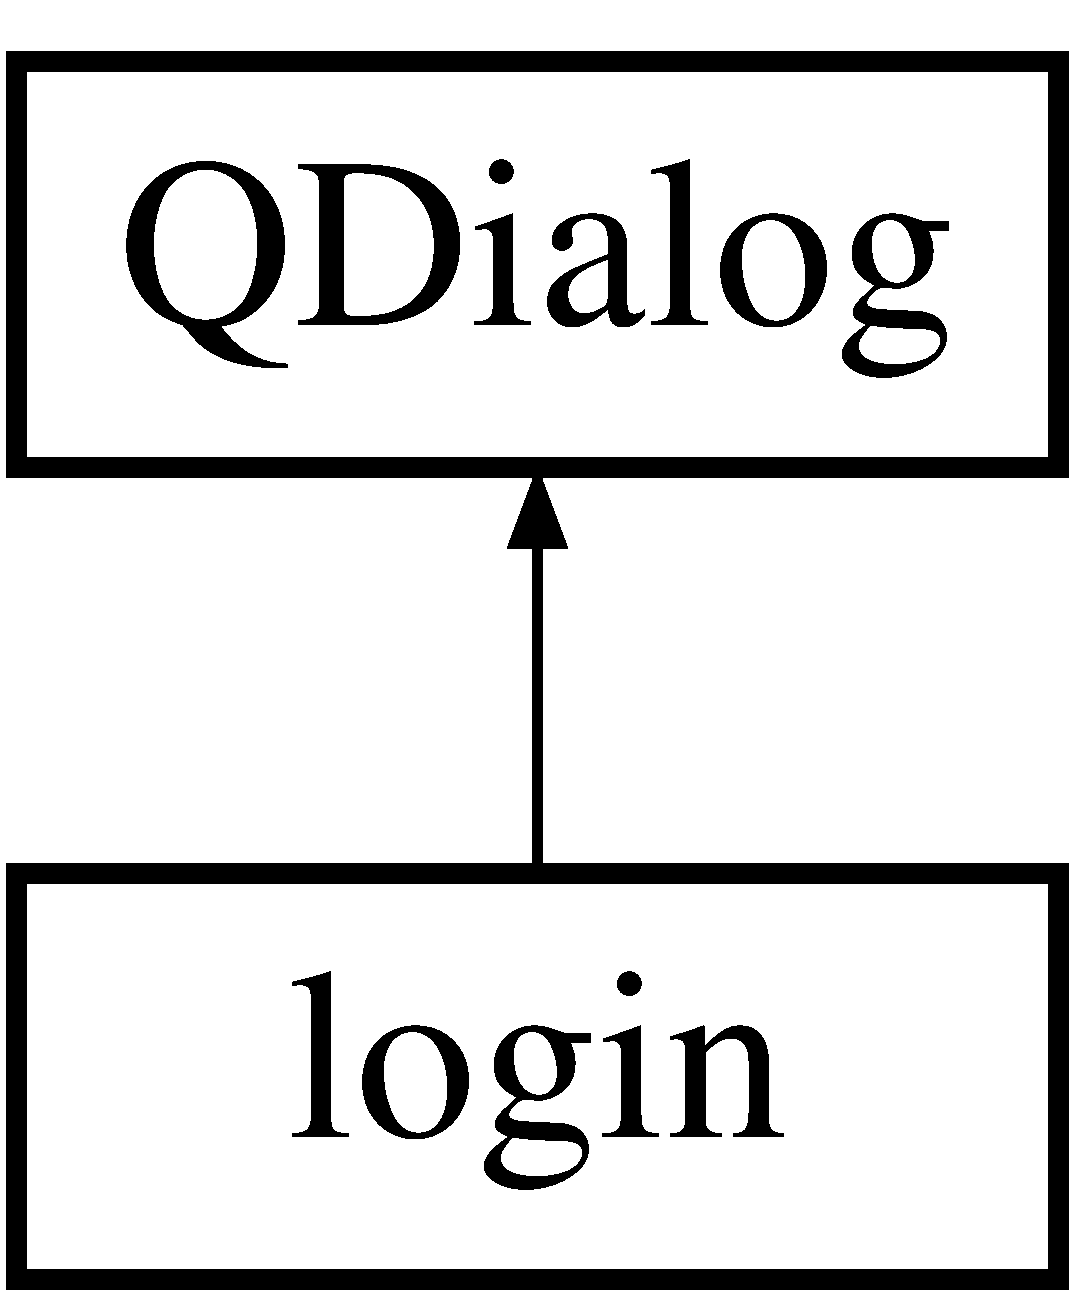
\includegraphics[height=2.000000cm]{classlogin}
\end{center}
\end{figure}
\subsection*{Public Member Functions}
\begin{DoxyCompactItemize}
\item 
\hyperlink{classlogin_a4bea95f394a7f5709d79b13455881602}{login} (Q\-Widget $\ast$parent=0)
\item 
int \hyperlink{classlogin_a42f5740b1023557256c4877abbb6e30d}{confirm\-User} (Q\-String username, Q\-String password)
\item 
int \hyperlink{classlogin_a1a62aa506d3b5e64710a74fc5b9a4beb}{add\-User} (Q\-String username, Q\-String password, int access\-Level)
\item 
\hyperlink{classlogin_a4086fe44ad1e40447a0bebbc9b8b3c14}{$\sim$login} ()
\end{DoxyCompactItemize}


\subsection{Detailed Description}
Login Class -\/ holds information for the user login dialog

\begin{DoxyAuthor}{Author}
richard (5/14/18) 
\end{DoxyAuthor}


\subsection{Constructor \& Destructor Documentation}
\hypertarget{classlogin_a4bea95f394a7f5709d79b13455881602}{\index{login@{login}!login@{login}}
\index{login@{login}!login@{login}}
\subsubsection[{login}]{\setlength{\rightskip}{0pt plus 5cm}login\-::login (
\begin{DoxyParamCaption}
\item[{Q\-Widget $\ast$}]{parent = {\ttfamily 0}}
\end{DoxyParamCaption}
)\hspace{0.3cm}{\ttfamily [explicit]}}}\label{classlogin_a4bea95f394a7f5709d79b13455881602}
contact constructor -\/ requires a Qwidgit to draw on

\begin{DoxyAuthor}{Author}
richard (5/13/18)
\end{DoxyAuthor}

\begin{DoxyParams}{Parameters}
{\em parent} & \\
\hline
\end{DoxyParams}
\hypertarget{classlogin_a4086fe44ad1e40447a0bebbc9b8b3c14}{\index{login@{login}!$\sim$login@{$\sim$login}}
\index{$\sim$login@{$\sim$login}!login@{login}}
\subsubsection[{$\sim$login}]{\setlength{\rightskip}{0pt plus 5cm}login\-::$\sim$login (
\begin{DoxyParamCaption}
{}
\end{DoxyParamCaption}
)}}\label{classlogin_a4086fe44ad1e40447a0bebbc9b8b3c14}
login destructor -\/ release allocated space

\begin{DoxyAuthor}{Author}
richard (5/14/18) 
\end{DoxyAuthor}


\subsection{Member Function Documentation}
\hypertarget{classlogin_a1a62aa506d3b5e64710a74fc5b9a4beb}{\index{login@{login}!add\-User@{add\-User}}
\index{add\-User@{add\-User}!login@{login}}
\subsubsection[{add\-User}]{\setlength{\rightskip}{0pt plus 5cm}int login\-::add\-User (
\begin{DoxyParamCaption}
\item[{Q\-String}]{username, }
\item[{Q\-String}]{password, }
\item[{int}]{access\-Level}
\end{DoxyParamCaption}
)}}\label{classlogin_a1a62aa506d3b5e64710a74fc5b9a4beb}
add\-User -\/ Checks if there are any duplicate usernames in file
\begin{DoxyItemize}
\item Appends user information into the file
\end{DoxyItemize}

\begin{DoxyAuthor}{Author}
richard (5/14/18)
\end{DoxyAuthor}

\begin{DoxyParams}{Parameters}
{\em username} & \\
\hline
{\em password} & \\
\hline
{\em access\-Level} & \\
\hline
\end{DoxyParams}
\begin{DoxyReturn}{Returns}
int 0 = no file found; 1= duplicate information (reenter); 2 = Valid/\-O\-K 
\end{DoxyReturn}
\hypertarget{classlogin_a42f5740b1023557256c4877abbb6e30d}{\index{login@{login}!confirm\-User@{confirm\-User}}
\index{confirm\-User@{confirm\-User}!login@{login}}
\subsubsection[{confirm\-User}]{\setlength{\rightskip}{0pt plus 5cm}int login\-::confirm\-User (
\begin{DoxyParamCaption}
\item[{Q\-String}]{username, }
\item[{Q\-String}]{password}
\end{DoxyParamCaption}
)}}\label{classlogin_a42f5740b1023557256c4877abbb6e30d}
confirm\-User -\/ Confirms if user and password is a matching pair in file

\begin{DoxyAuthor}{Author}
richard (5/14/18)
\end{DoxyAuthor}

\begin{DoxyParams}{Parameters}
{\em username} & \\
\hline
{\em password} & \\
\hline
\end{DoxyParams}
\begin{DoxyReturn}{Returns}
int 0 = Invalid user; 1 = guest user; 2 = administrator 
\end{DoxyReturn}


The documentation for this class was generated from the following files\-:\begin{DoxyCompactItemize}
\item 
/home/edt/\-C\-S1\-C/\-Class\-Project/\-Main\-Window/login.\-h\item 
/home/edt/\-C\-S1\-C/\-Class\-Project/\-Main\-Window/login.\-cpp\end{DoxyCompactItemize}

\hypertarget{classMainWindow}{\section{Main\-Window Class Reference}
\label{classMainWindow}\index{Main\-Window@{Main\-Window}}
}
Inheritance diagram for Main\-Window\-:\begin{figure}[H]
\begin{center}
\leavevmode
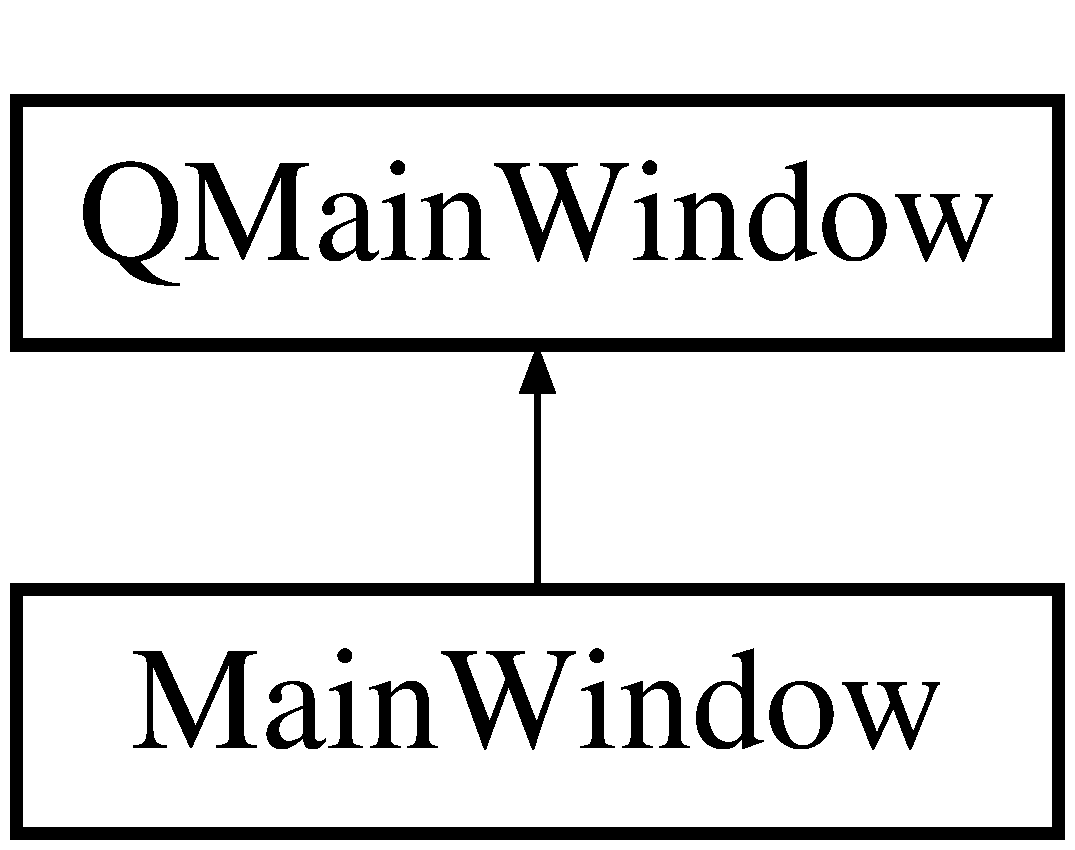
\includegraphics[height=2.000000cm]{classMainWindow}
\end{center}
\end{figure}
\subsection*{Public Types}
\begin{DoxyCompactItemize}
\item 
enum {\bfseries base} \{ {\bfseries base\-Select}, 
{\bfseries base\-Line}, 
{\bfseries base2\-D}, 
{\bfseries base\-Text}
 \}
\end{DoxyCompactItemize}
\subsection*{Public Member Functions}
\begin{DoxyCompactItemize}
\item 
\hypertarget{classMainWindow_a8b244be8b7b7db1b08de2a2acb9409db}{{\bfseries Main\-Window} (Q\-Widget $\ast$parent=0)}\label{classMainWindow_a8b244be8b7b7db1b08de2a2acb9409db}

\item 
\hypertarget{classMainWindow_a5fb4bbae0c6be3fcc88900c8956173db}{void {\bfseries set\-Vector} (\hyperlink{classnserkkvector_1_1MyVector}{My\-Vector}$<$ \hyperlink{classShape}{Shape} $\ast$ $>$ $\ast$temp)}\label{classMainWindow_a5fb4bbae0c6be3fcc88900c8956173db}

\item 
\hypertarget{classMainWindow_a4205e879c75cff5f992f0f9c9accffc7}{void {\bfseries reload\-Vector} ()}\label{classMainWindow_a4205e879c75cff5f992f0f9c9accffc7}

\item 
\hypertarget{classMainWindow_a3dfe834b2836b316908ace3f38c06db2}{void {\bfseries show\-Event} (Q\-Show\-Event $\ast$event)}\label{classMainWindow_a3dfe834b2836b316908ace3f38c06db2}

\item 
\hypertarget{classMainWindow_afb9c74c4702c602f4b60e669b76cf339}{void {\bfseries combo\-Box\-Base\-Shape} (int index, base \&cur\-Shape)}\label{classMainWindow_afb9c74c4702c602f4b60e669b76cf339}

\item 
\hypertarget{classMainWindow_af54a660c334cabf6add34d5e8c048cc1}{int {\bfseries parse\-Pen\-Color} (Q\-Color color)}\label{classMainWindow_af54a660c334cabf6add34d5e8c048cc1}

\item 
\hypertarget{classMainWindow_a82e285c2886a18a76aa0ed47c45ab566}{int {\bfseries parse\-Pen\-Style} (int counter)}\label{classMainWindow_a82e285c2886a18a76aa0ed47c45ab566}

\item 
\hypertarget{classMainWindow_a24fc2fa76e0d386c0562947b55786129}{void {\bfseries update\-Add\-Tab} ()}\label{classMainWindow_a24fc2fa76e0d386c0562947b55786129}

\item 
\hypertarget{classMainWindow_a9c5df82c43a4ef712a17e8f8503f2cc8}{void {\bfseries update\-Mod\-Tab} ()}\label{classMainWindow_a9c5df82c43a4ef712a17e8f8503f2cc8}

\end{DoxyCompactItemize}
\subsection*{Public Attributes}
\begin{DoxyCompactItemize}
\item 
\hypertarget{classMainWindow_aae71fe8e7810224f27c78b6417f46606}{enum Main\-Window\-::base {\bfseries mod\-Cur\-Shape}}\label{classMainWindow_aae71fe8e7810224f27c78b6417f46606}

\item 
\hypertarget{classMainWindow_afb1baef08726f6699edc677c29418560}{enum Main\-Window\-::base {\bfseries add\-Cur\-Shape}}\label{classMainWindow_afb1baef08726f6699edc677c29418560}

\end{DoxyCompactItemize}


The documentation for this class was generated from the following files\-:\begin{DoxyCompactItemize}
\item 
/home/edt/\-C\-S1\-C/\-Class\-Project/\-Main\-Window/mainwindow.\-h\item 
/home/edt/\-C\-S1\-C/\-Class\-Project/\-Main\-Window/mainwindow.\-cpp\end{DoxyCompactItemize}

\hypertarget{classnserkkvector_1_1MyVector}{\section{nserkkvector\-:\-:My\-Vector$<$ T $>$ Class Template Reference}
\label{classnserkkvector_1_1MyVector}\index{nserkkvector\-::\-My\-Vector$<$ T $>$@{nserkkvector\-::\-My\-Vector$<$ T $>$}}
}


{\ttfamily \#include $<$vector.\-h$>$}

\subsection*{Public Types}
\begin{DoxyCompactItemize}
\item 
\hypertarget{classnserkkvector_1_1MyVector_af2532d112ac2aba9021f39363b0bcc85}{using {\bfseries iterator} = T $\ast$}\label{classnserkkvector_1_1MyVector_af2532d112ac2aba9021f39363b0bcc85}

\item 
\hypertarget{classnserkkvector_1_1MyVector_a86745c2740ee00848df38e9c38d9d1d2}{using {\bfseries const\-\_\-iterator} = const T $\ast$}\label{classnserkkvector_1_1MyVector_a86745c2740ee00848df38e9c38d9d1d2}

\end{DoxyCompactItemize}
\subsection*{Public Member Functions}
\begin{DoxyCompactItemize}
\item 
\hyperlink{classnserkkvector_1_1MyVector_a08c4f3b0452a7b948575be6e314fb1e5}{My\-Vector} ()
\item 
\hyperlink{classnserkkvector_1_1MyVector_a28304d57842aa7d53c82f1dc1609571a}{My\-Vector} (int alloc\-\_\-size, T \&fill\-Elem=T())
\item 
\hyperlink{classnserkkvector_1_1MyVector_a3a6a68ac048925dd90787c4ef7394d9d}{My\-Vector} (const \hyperlink{classnserkkvector_1_1MyVector}{My\-Vector}$<$ T $>$ \&src)
\item 
\hyperlink{classnserkkvector_1_1MyVector}{My\-Vector} \& \hyperlink{classnserkkvector_1_1MyVector_a2fb5d92fbe96180a02000e26b74e2322}{operator=} (const \hyperlink{classnserkkvector_1_1MyVector}{My\-Vector} \&rhs)
\item 
\hyperlink{classnserkkvector_1_1MyVector_ad9756f4689fe2b67b7b90ae54352d537}{$\sim$\-My\-Vector} ()
\item 
iterator \hyperlink{classnserkkvector_1_1MyVector_acbc69c4ebe8b558f2501288defc408f3}{begin} ()
\item 
const\-\_\-iterator \hyperlink{classnserkkvector_1_1MyVector_a75db7328d5f9b832ddefc5b150400b31}{begin} () const 
\item 
iterator \hyperlink{classnserkkvector_1_1MyVector_a7d9303b06eef419159d069a04b14aa62}{end} ()
\item 
const\-\_\-iterator \hyperlink{classnserkkvector_1_1MyVector_a02b21caae0eb09bb743da7a0377332a7}{end} () const 
\item 
void \hyperlink{classnserkkvector_1_1MyVector_adcd5abe3736336323650ac82177a735b}{reserve} (int alloc\-\_\-size)
\item 
iterator \hyperlink{classnserkkvector_1_1MyVector_af4dabeb13a9f939dbac185e8612a9c97}{insert} (iterator position, const T \&newval)
\item 
iterator \hyperlink{classnserkkvector_1_1MyVector_a1277bd066bb9d1c4710de998c8c1794a}{erase} (iterator position)
\item 
T \hyperlink{classnserkkvector_1_1MyVector_a701323e9da33aba5e3177e9a5bfe9d8c}{operator\mbox{[}$\,$\mbox{]}} (int n)
\item 
const T \& \hyperlink{classnserkkvector_1_1MyVector_a541e75a1fe77de2ec8e4d3b01e71a8de}{operator\mbox{[}$\,$\mbox{]}} (int n) const 
\item 
int \hyperlink{classnserkkvector_1_1MyVector_ad13ecb704153390b12149a5fb620bec6}{size} () const 
\item 
int \hyperlink{classnserkkvector_1_1MyVector_adf37bc0a5ec865e90a26653fce8168fc}{capacity} () const 
\item 
void \hyperlink{classnserkkvector_1_1MyVector_a1ba1aa4622327c812e5fe82babdae347}{resize} (int alloc\-\_\-size)
\item 
void \hyperlink{classnserkkvector_1_1MyVector_ade60c7713d1fd226e64ee208e00a0f53}{push\-\_\-back} (const T \&new\-\_\-elem)
\item 
void \hyperlink{classnserkkvector_1_1MyVector_a5a329025df9d93fba598208961e2b9c6}{print\-As\-Debug} (bool printeol, bool printcontent) const 
\end{DoxyCompactItemize}


\subsection{Detailed Description}
\subsubsection*{template$<$class T$>$class nserkkvector\-::\-My\-Vector$<$ T $>$}

\hyperlink{classnserkkvector_1_1MyVector}{My\-Vector} -\/ minimal vector class -\/ partial implementation of S\-T\-L vector

\begin{DoxyAuthor}{Author}
edt (5/14/18) 
\end{DoxyAuthor}


\subsection{Constructor \& Destructor Documentation}
\hypertarget{classnserkkvector_1_1MyVector_a08c4f3b0452a7b948575be6e314fb1e5}{\index{nserkkvector\-::\-My\-Vector@{nserkkvector\-::\-My\-Vector}!My\-Vector@{My\-Vector}}
\index{My\-Vector@{My\-Vector}!nserkkvector::MyVector@{nserkkvector\-::\-My\-Vector}}
\subsubsection[{My\-Vector}]{\setlength{\rightskip}{0pt plus 5cm}template$<$class T$>$ {\bf nserkkvector\-::\-My\-Vector}$<$ T $>$\-::{\bf My\-Vector} (
\begin{DoxyParamCaption}
{}
\end{DoxyParamCaption}
)\hspace{0.3cm}{\ttfamily [inline]}}}\label{classnserkkvector_1_1MyVector_a08c4f3b0452a7b948575be6e314fb1e5}
\hyperlink{classnserkkvector_1_1MyVector}{My\-Vector} default constructor -\/ create an empty vector

\begin{DoxyAuthor}{Author}
edt (5/14/18) 
\end{DoxyAuthor}
\hypertarget{classnserkkvector_1_1MyVector_a28304d57842aa7d53c82f1dc1609571a}{\index{nserkkvector\-::\-My\-Vector@{nserkkvector\-::\-My\-Vector}!My\-Vector@{My\-Vector}}
\index{My\-Vector@{My\-Vector}!nserkkvector::MyVector@{nserkkvector\-::\-My\-Vector}}
\subsubsection[{My\-Vector}]{\setlength{\rightskip}{0pt plus 5cm}template$<$class T$>$ {\bf nserkkvector\-::\-My\-Vector}$<$ T $>$\-::{\bf My\-Vector} (
\begin{DoxyParamCaption}
\item[{int}]{alloc\-\_\-size, }
\item[{T \&}]{fill\-Elem = {\ttfamily T()}}
\end{DoxyParamCaption}
)\hspace{0.3cm}{\ttfamily [inline]}, {\ttfamily [explicit]}}}\label{classnserkkvector_1_1MyVector_a28304d57842aa7d53c82f1dc1609571a}
\hyperlink{classnserkkvector_1_1MyVector}{My\-Vector} constructor -\/ create a vector of specified size

\begin{DoxyAuthor}{Author}
edt (5/14/18)
\end{DoxyAuthor}

\begin{DoxyParams}{Parameters}
{\em size} & -\/ number of elements -\/1 that vector may contain \\
\hline
{\em fill\-Elem} & -\/ sample element to put in each entry in vector \\
\hline
\end{DoxyParams}
\hypertarget{classnserkkvector_1_1MyVector_a3a6a68ac048925dd90787c4ef7394d9d}{\index{nserkkvector\-::\-My\-Vector@{nserkkvector\-::\-My\-Vector}!My\-Vector@{My\-Vector}}
\index{My\-Vector@{My\-Vector}!nserkkvector::MyVector@{nserkkvector\-::\-My\-Vector}}
\subsubsection[{My\-Vector}]{\setlength{\rightskip}{0pt plus 5cm}template$<$class T$>$ {\bf nserkkvector\-::\-My\-Vector}$<$ T $>$\-::{\bf My\-Vector} (
\begin{DoxyParamCaption}
\item[{const {\bf My\-Vector}$<$ T $>$ \&}]{src}
\end{DoxyParamCaption}
)\hspace{0.3cm}{\ttfamily [inline]}}}\label{classnserkkvector_1_1MyVector_a3a6a68ac048925dd90787c4ef7394d9d}
\hyperlink{classnserkkvector_1_1MyVector}{My\-Vector} copy constructor

\begin{DoxyAuthor}{Author}
edt (5/14/18)
\end{DoxyAuthor}

\begin{DoxyParams}{Parameters}
{\em src\&amp;} & -\/ vector to copy elements from \\
\hline
\end{DoxyParams}
\hypertarget{classnserkkvector_1_1MyVector_ad9756f4689fe2b67b7b90ae54352d537}{\index{nserkkvector\-::\-My\-Vector@{nserkkvector\-::\-My\-Vector}!$\sim$\-My\-Vector@{$\sim$\-My\-Vector}}
\index{$\sim$\-My\-Vector@{$\sim$\-My\-Vector}!nserkkvector::MyVector@{nserkkvector\-::\-My\-Vector}}
\subsubsection[{$\sim$\-My\-Vector}]{\setlength{\rightskip}{0pt plus 5cm}template$<$class T$>$ {\bf nserkkvector\-::\-My\-Vector}$<$ T $>$\-::$\sim${\bf My\-Vector} (
\begin{DoxyParamCaption}
{}
\end{DoxyParamCaption}
)\hspace{0.3cm}{\ttfamily [inline]}}}\label{classnserkkvector_1_1MyVector_ad9756f4689fe2b67b7b90ae54352d537}
Destructor -\/ simply free the object space and array of elements

\begin{DoxyAuthor}{Author}
edt (5/13/18) 
\end{DoxyAuthor}


\subsection{Member Function Documentation}
\hypertarget{classnserkkvector_1_1MyVector_acbc69c4ebe8b558f2501288defc408f3}{\index{nserkkvector\-::\-My\-Vector@{nserkkvector\-::\-My\-Vector}!begin@{begin}}
\index{begin@{begin}!nserkkvector::MyVector@{nserkkvector\-::\-My\-Vector}}
\subsubsection[{begin}]{\setlength{\rightskip}{0pt plus 5cm}template$<$class T$>$ iterator {\bf nserkkvector\-::\-My\-Vector}$<$ T $>$\-::begin (
\begin{DoxyParamCaption}
{}
\end{DoxyParamCaption}
)\hspace{0.3cm}{\ttfamily [inline]}}}\label{classnserkkvector_1_1MyVector_acbc69c4ebe8b558f2501288defc408f3}
\hyperlink{classnserkkvector_1_1MyVector}{My\-Vector} iterator -\/ get first element address

\begin{DoxyAuthor}{Author}
edt (5/14/18)
\end{DoxyAuthor}
\begin{DoxyReturn}{Returns}
pointer to first element 
\end{DoxyReturn}
\hypertarget{classnserkkvector_1_1MyVector_a75db7328d5f9b832ddefc5b150400b31}{\index{nserkkvector\-::\-My\-Vector@{nserkkvector\-::\-My\-Vector}!begin@{begin}}
\index{begin@{begin}!nserkkvector::MyVector@{nserkkvector\-::\-My\-Vector}}
\subsubsection[{begin}]{\setlength{\rightskip}{0pt plus 5cm}template$<$class T$>$ const\-\_\-iterator {\bf nserkkvector\-::\-My\-Vector}$<$ T $>$\-::begin (
\begin{DoxyParamCaption}
{}
\end{DoxyParamCaption}
) const\hspace{0.3cm}{\ttfamily [inline]}}}\label{classnserkkvector_1_1MyVector_a75db7328d5f9b832ddefc5b150400b31}
\hyperlink{classnserkkvector_1_1MyVector}{My\-Vector} iterator -\/ get first element address -\/ const

\begin{DoxyAuthor}{Author}
edt (5/14/18)
\end{DoxyAuthor}
\begin{DoxyReturn}{Returns}
pointer to const first element 
\end{DoxyReturn}
\hypertarget{classnserkkvector_1_1MyVector_adf37bc0a5ec865e90a26653fce8168fc}{\index{nserkkvector\-::\-My\-Vector@{nserkkvector\-::\-My\-Vector}!capacity@{capacity}}
\index{capacity@{capacity}!nserkkvector::MyVector@{nserkkvector\-::\-My\-Vector}}
\subsubsection[{capacity}]{\setlength{\rightskip}{0pt plus 5cm}template$<$class T$>$ int {\bf nserkkvector\-::\-My\-Vector}$<$ T $>$\-::capacity (
\begin{DoxyParamCaption}
{}
\end{DoxyParamCaption}
) const\hspace{0.3cm}{\ttfamily [inline]}}}\label{classnserkkvector_1_1MyVector_adf37bc0a5ec865e90a26653fce8168fc}
capacity -\/ return number of possible elements in the vector + 1

\begin{DoxyAuthor}{Author}
edt (5/14/18)
\end{DoxyAuthor}
\begin{DoxyReturn}{Returns}
int 
\end{DoxyReturn}
\hypertarget{classnserkkvector_1_1MyVector_a7d9303b06eef419159d069a04b14aa62}{\index{nserkkvector\-::\-My\-Vector@{nserkkvector\-::\-My\-Vector}!end@{end}}
\index{end@{end}!nserkkvector::MyVector@{nserkkvector\-::\-My\-Vector}}
\subsubsection[{end}]{\setlength{\rightskip}{0pt plus 5cm}template$<$class T$>$ iterator {\bf nserkkvector\-::\-My\-Vector}$<$ T $>$\-::end (
\begin{DoxyParamCaption}
{}
\end{DoxyParamCaption}
)\hspace{0.3cm}{\ttfamily [inline]}}}\label{classnserkkvector_1_1MyVector_a7d9303b06eef419159d069a04b14aa62}
\hyperlink{classnserkkvector_1_1MyVector}{My\-Vector} iterator -\/ get last element address

\begin{DoxyAuthor}{Author}
edt (5/14/18)
\end{DoxyAuthor}
\begin{DoxyReturn}{Returns}
pointer to last element 
\end{DoxyReturn}
\hypertarget{classnserkkvector_1_1MyVector_a02b21caae0eb09bb743da7a0377332a7}{\index{nserkkvector\-::\-My\-Vector@{nserkkvector\-::\-My\-Vector}!end@{end}}
\index{end@{end}!nserkkvector::MyVector@{nserkkvector\-::\-My\-Vector}}
\subsubsection[{end}]{\setlength{\rightskip}{0pt plus 5cm}template$<$class T$>$ const\-\_\-iterator {\bf nserkkvector\-::\-My\-Vector}$<$ T $>$\-::end (
\begin{DoxyParamCaption}
{}
\end{DoxyParamCaption}
) const\hspace{0.3cm}{\ttfamily [inline]}}}\label{classnserkkvector_1_1MyVector_a02b21caae0eb09bb743da7a0377332a7}
\hyperlink{classnserkkvector_1_1MyVector}{My\-Vector} iterator -\/ get last element address -\/ const

\begin{DoxyAuthor}{Author}
edt (5/14/18)
\end{DoxyAuthor}
\begin{DoxyReturn}{Returns}
pointer to const lst element 
\end{DoxyReturn}
\hypertarget{classnserkkvector_1_1MyVector_a1277bd066bb9d1c4710de998c8c1794a}{\index{nserkkvector\-::\-My\-Vector@{nserkkvector\-::\-My\-Vector}!erase@{erase}}
\index{erase@{erase}!nserkkvector::MyVector@{nserkkvector\-::\-My\-Vector}}
\subsubsection[{erase}]{\setlength{\rightskip}{0pt plus 5cm}template$<$class T$>$ iterator {\bf nserkkvector\-::\-My\-Vector}$<$ T $>$\-::erase (
\begin{DoxyParamCaption}
\item[{iterator}]{position}
\end{DoxyParamCaption}
)\hspace{0.3cm}{\ttfamily [inline]}}}\label{classnserkkvector_1_1MyVector_a1277bd066bb9d1c4710de998c8c1794a}
erase -\/ remove element specifieed

\begin{DoxyAuthor}{Author}
edt (5/14/18)
\end{DoxyAuthor}

\begin{DoxyParams}{Parameters}
{\em position} & -\/ location of element to delete\\
\hline
\end{DoxyParams}
\begin{DoxyReturn}{Returns}
iterator\& -\/ location of element now at specified location 
\end{DoxyReturn}
\hypertarget{classnserkkvector_1_1MyVector_af4dabeb13a9f939dbac185e8612a9c97}{\index{nserkkvector\-::\-My\-Vector@{nserkkvector\-::\-My\-Vector}!insert@{insert}}
\index{insert@{insert}!nserkkvector::MyVector@{nserkkvector\-::\-My\-Vector}}
\subsubsection[{insert}]{\setlength{\rightskip}{0pt plus 5cm}template$<$class T$>$ iterator {\bf nserkkvector\-::\-My\-Vector}$<$ T $>$\-::insert (
\begin{DoxyParamCaption}
\item[{iterator}]{position, }
\item[{const T \&}]{newval}
\end{DoxyParamCaption}
)\hspace{0.3cm}{\ttfamily [inline]}}}\label{classnserkkvector_1_1MyVector_af4dabeb13a9f939dbac185e8612a9c97}
insert -\/ place new element into vector before element specified by iterator

\begin{DoxyAuthor}{Author}
edt (5/14/18)
\end{DoxyAuthor}

\begin{DoxyParams}{Parameters}
{\em position} & -\/ location before which to insert new element \\
\hline
{\em newval} & -\/ element to insert\\
\hline
\end{DoxyParams}
\begin{DoxyReturn}{Returns}
iterator\& -\/ location of new element 
\end{DoxyReturn}
\hypertarget{classnserkkvector_1_1MyVector_a2fb5d92fbe96180a02000e26b74e2322}{\index{nserkkvector\-::\-My\-Vector@{nserkkvector\-::\-My\-Vector}!operator=@{operator=}}
\index{operator=@{operator=}!nserkkvector::MyVector@{nserkkvector\-::\-My\-Vector}}
\subsubsection[{operator=}]{\setlength{\rightskip}{0pt plus 5cm}template$<$class T$>$ {\bf My\-Vector}\& {\bf nserkkvector\-::\-My\-Vector}$<$ T $>$\-::operator= (
\begin{DoxyParamCaption}
\item[{const {\bf My\-Vector}$<$ T $>$ \&}]{rhs}
\end{DoxyParamCaption}
)\hspace{0.3cm}{\ttfamily [inline]}}}\label{classnserkkvector_1_1MyVector_a2fb5d92fbe96180a02000e26b74e2322}
\hyperlink{classnserkkvector_1_1MyVector}{My\-Vector} copy constructor

\begin{DoxyAuthor}{Author}
edt (5/14/18)
\end{DoxyAuthor}

\begin{DoxyParams}{Parameters}
{\em rhs\&amp;} & -\/ vector to copy elements from\\
\hline
\end{DoxyParams}
\begin{DoxyReturn}{Returns}
\hyperlink{classnserkkvector_1_1MyVector}{My\-Vector}\& 
\end{DoxyReturn}
\hypertarget{classnserkkvector_1_1MyVector_a701323e9da33aba5e3177e9a5bfe9d8c}{\index{nserkkvector\-::\-My\-Vector@{nserkkvector\-::\-My\-Vector}!operator\mbox{[}$\,$\mbox{]}@{operator[]}}
\index{operator\mbox{[}$\,$\mbox{]}@{operator[]}!nserkkvector::MyVector@{nserkkvector\-::\-My\-Vector}}
\subsubsection[{operator[]}]{\setlength{\rightskip}{0pt plus 5cm}template$<$class T$>$ T {\bf nserkkvector\-::\-My\-Vector}$<$ T $>$\-::operator\mbox{[}$\,$\mbox{]} (
\begin{DoxyParamCaption}
\item[{int}]{n}
\end{DoxyParamCaption}
)\hspace{0.3cm}{\ttfamily [inline]}}}\label{classnserkkvector_1_1MyVector_a701323e9da33aba5e3177e9a5bfe9d8c}
operator\mbox{[}\mbox{]} -\/ return pointer to specified element

\begin{DoxyAuthor}{Author}
edt (5/14/18)
\end{DoxyAuthor}

\begin{DoxyParams}{Parameters}
{\em n} & -\/ element number (0 based) to return\\
\hline
\end{DoxyParams}
\begin{DoxyReturn}{Returns}
iterator\& -\/ location of element at specified location 
\end{DoxyReturn}
\hypertarget{classnserkkvector_1_1MyVector_a541e75a1fe77de2ec8e4d3b01e71a8de}{\index{nserkkvector\-::\-My\-Vector@{nserkkvector\-::\-My\-Vector}!operator\mbox{[}$\,$\mbox{]}@{operator[]}}
\index{operator\mbox{[}$\,$\mbox{]}@{operator[]}!nserkkvector::MyVector@{nserkkvector\-::\-My\-Vector}}
\subsubsection[{operator[]}]{\setlength{\rightskip}{0pt plus 5cm}template$<$class T$>$ const T\& {\bf nserkkvector\-::\-My\-Vector}$<$ T $>$\-::operator\mbox{[}$\,$\mbox{]} (
\begin{DoxyParamCaption}
\item[{int}]{n}
\end{DoxyParamCaption}
) const\hspace{0.3cm}{\ttfamily [inline]}}}\label{classnserkkvector_1_1MyVector_a541e75a1fe77de2ec8e4d3b01e71a8de}
operator\mbox{[}\mbox{]} -\/ return pointer to specified element -\/ pointer to const

\begin{DoxyAuthor}{Author}
edt (5/14/18)
\end{DoxyAuthor}

\begin{DoxyParams}{Parameters}
{\em n} & -\/ element number (0 based) to return\\
\hline
\end{DoxyParams}
\begin{DoxyReturn}{Returns}
iterator\& -\/ location of element at specified location 
\end{DoxyReturn}
\hypertarget{classnserkkvector_1_1MyVector_a5a329025df9d93fba598208961e2b9c6}{\index{nserkkvector\-::\-My\-Vector@{nserkkvector\-::\-My\-Vector}!print\-As\-Debug@{print\-As\-Debug}}
\index{print\-As\-Debug@{print\-As\-Debug}!nserkkvector::MyVector@{nserkkvector\-::\-My\-Vector}}
\subsubsection[{print\-As\-Debug}]{\setlength{\rightskip}{0pt plus 5cm}template$<$class T$>$ void {\bf nserkkvector\-::\-My\-Vector}$<$ T $>$\-::print\-As\-Debug (
\begin{DoxyParamCaption}
\item[{bool}]{printeol, }
\item[{bool}]{printcontent}
\end{DoxyParamCaption}
) const\hspace{0.3cm}{\ttfamily [inline]}}}\label{classnserkkvector_1_1MyVector_a5a329025df9d93fba598208961e2b9c6}
print\-As\-Debug -\/ print control structures and elements, if desired for debugging

\begin{DoxyAuthor}{Author}
edt (5/14/18)
\end{DoxyAuthor}

\begin{DoxyParams}{Parameters}
{\em printeol} & -\/ print end of line after each feild/element being printed \\
\hline
{\em printcontent} & -\/ print information about elements in the vector \\
\hline
\end{DoxyParams}
\hypertarget{classnserkkvector_1_1MyVector_ade60c7713d1fd226e64ee208e00a0f53}{\index{nserkkvector\-::\-My\-Vector@{nserkkvector\-::\-My\-Vector}!push\-\_\-back@{push\-\_\-back}}
\index{push\-\_\-back@{push\-\_\-back}!nserkkvector::MyVector@{nserkkvector\-::\-My\-Vector}}
\subsubsection[{push\-\_\-back}]{\setlength{\rightskip}{0pt plus 5cm}template$<$class T$>$ void {\bf nserkkvector\-::\-My\-Vector}$<$ T $>$\-::push\-\_\-back (
\begin{DoxyParamCaption}
\item[{const T \&}]{new\-\_\-elem}
\end{DoxyParamCaption}
)\hspace{0.3cm}{\ttfamily [inline]}}}\label{classnserkkvector_1_1MyVector_ade60c7713d1fd226e64ee208e00a0f53}
push\-\_\-back -\/ add element to end of vector -\/ resize if needed

\begin{DoxyAuthor}{Author}
edt (5/14/18)
\end{DoxyAuthor}

\begin{DoxyParams}{Parameters}
{\em alloc\-\_\-size} & -\/ number of elements desired -\/1 \\
\hline
\end{DoxyParams}
\hypertarget{classnserkkvector_1_1MyVector_adcd5abe3736336323650ac82177a735b}{\index{nserkkvector\-::\-My\-Vector@{nserkkvector\-::\-My\-Vector}!reserve@{reserve}}
\index{reserve@{reserve}!nserkkvector::MyVector@{nserkkvector\-::\-My\-Vector}}
\subsubsection[{reserve}]{\setlength{\rightskip}{0pt plus 5cm}template$<$class T$>$ void {\bf nserkkvector\-::\-My\-Vector}$<$ T $>$\-::reserve (
\begin{DoxyParamCaption}
\item[{int}]{alloc\-\_\-size}
\end{DoxyParamCaption}
)\hspace{0.3cm}{\ttfamily [inline]}}}\label{classnserkkvector_1_1MyVector_adcd5abe3736336323650ac82177a735b}
reserve -\/ allocate more space to vector

\begin{DoxyAuthor}{Author}
edt (5/14/18)
\end{DoxyAuthor}

\begin{DoxyParams}{Parameters}
{\em alloc\-\_\-size} & -\/ number of elements -\/1 that can be contained \\
\hline
\end{DoxyParams}
\hypertarget{classnserkkvector_1_1MyVector_a1ba1aa4622327c812e5fe82babdae347}{\index{nserkkvector\-::\-My\-Vector@{nserkkvector\-::\-My\-Vector}!resize@{resize}}
\index{resize@{resize}!nserkkvector::MyVector@{nserkkvector\-::\-My\-Vector}}
\subsubsection[{resize}]{\setlength{\rightskip}{0pt plus 5cm}template$<$class T$>$ void {\bf nserkkvector\-::\-My\-Vector}$<$ T $>$\-::resize (
\begin{DoxyParamCaption}
\item[{int}]{alloc\-\_\-size}
\end{DoxyParamCaption}
)\hspace{0.3cm}{\ttfamily [inline]}}}\label{classnserkkvector_1_1MyVector_a1ba1aa4622327c812e5fe82babdae347}
resize -\/ add storage to contain specified number of elements -\/ 1

\begin{DoxyAuthor}{Author}
edt (5/14/18)
\end{DoxyAuthor}

\begin{DoxyParams}{Parameters}
{\em alloc\-\_\-size} & -\/ number of elements desired -\/1 \\
\hline
\end{DoxyParams}
\hypertarget{classnserkkvector_1_1MyVector_ad13ecb704153390b12149a5fb620bec6}{\index{nserkkvector\-::\-My\-Vector@{nserkkvector\-::\-My\-Vector}!size@{size}}
\index{size@{size}!nserkkvector::MyVector@{nserkkvector\-::\-My\-Vector}}
\subsubsection[{size}]{\setlength{\rightskip}{0pt plus 5cm}template$<$class T$>$ int {\bf nserkkvector\-::\-My\-Vector}$<$ T $>$\-::size (
\begin{DoxyParamCaption}
{}
\end{DoxyParamCaption}
) const\hspace{0.3cm}{\ttfamily [inline]}}}\label{classnserkkvector_1_1MyVector_ad13ecb704153390b12149a5fb620bec6}
size -\/ return number of elements in the vector

\begin{DoxyAuthor}{Author}
edt (5/14/18)
\end{DoxyAuthor}
\begin{DoxyReturn}{Returns}
int 
\end{DoxyReturn}


The documentation for this class was generated from the following file\-:\begin{DoxyCompactItemize}
\item 
/home/edt/\-C\-S1\-C/\-Class\-Project/\-Main\-Window/vector.\-h\end{DoxyCompactItemize}

\hypertarget{classPolygon}{\section{Polygon Class Reference}
\label{classPolygon}\index{Polygon@{Polygon}}
}
Inheritance diagram for Polygon\-:\begin{figure}[H]
\begin{center}
\leavevmode
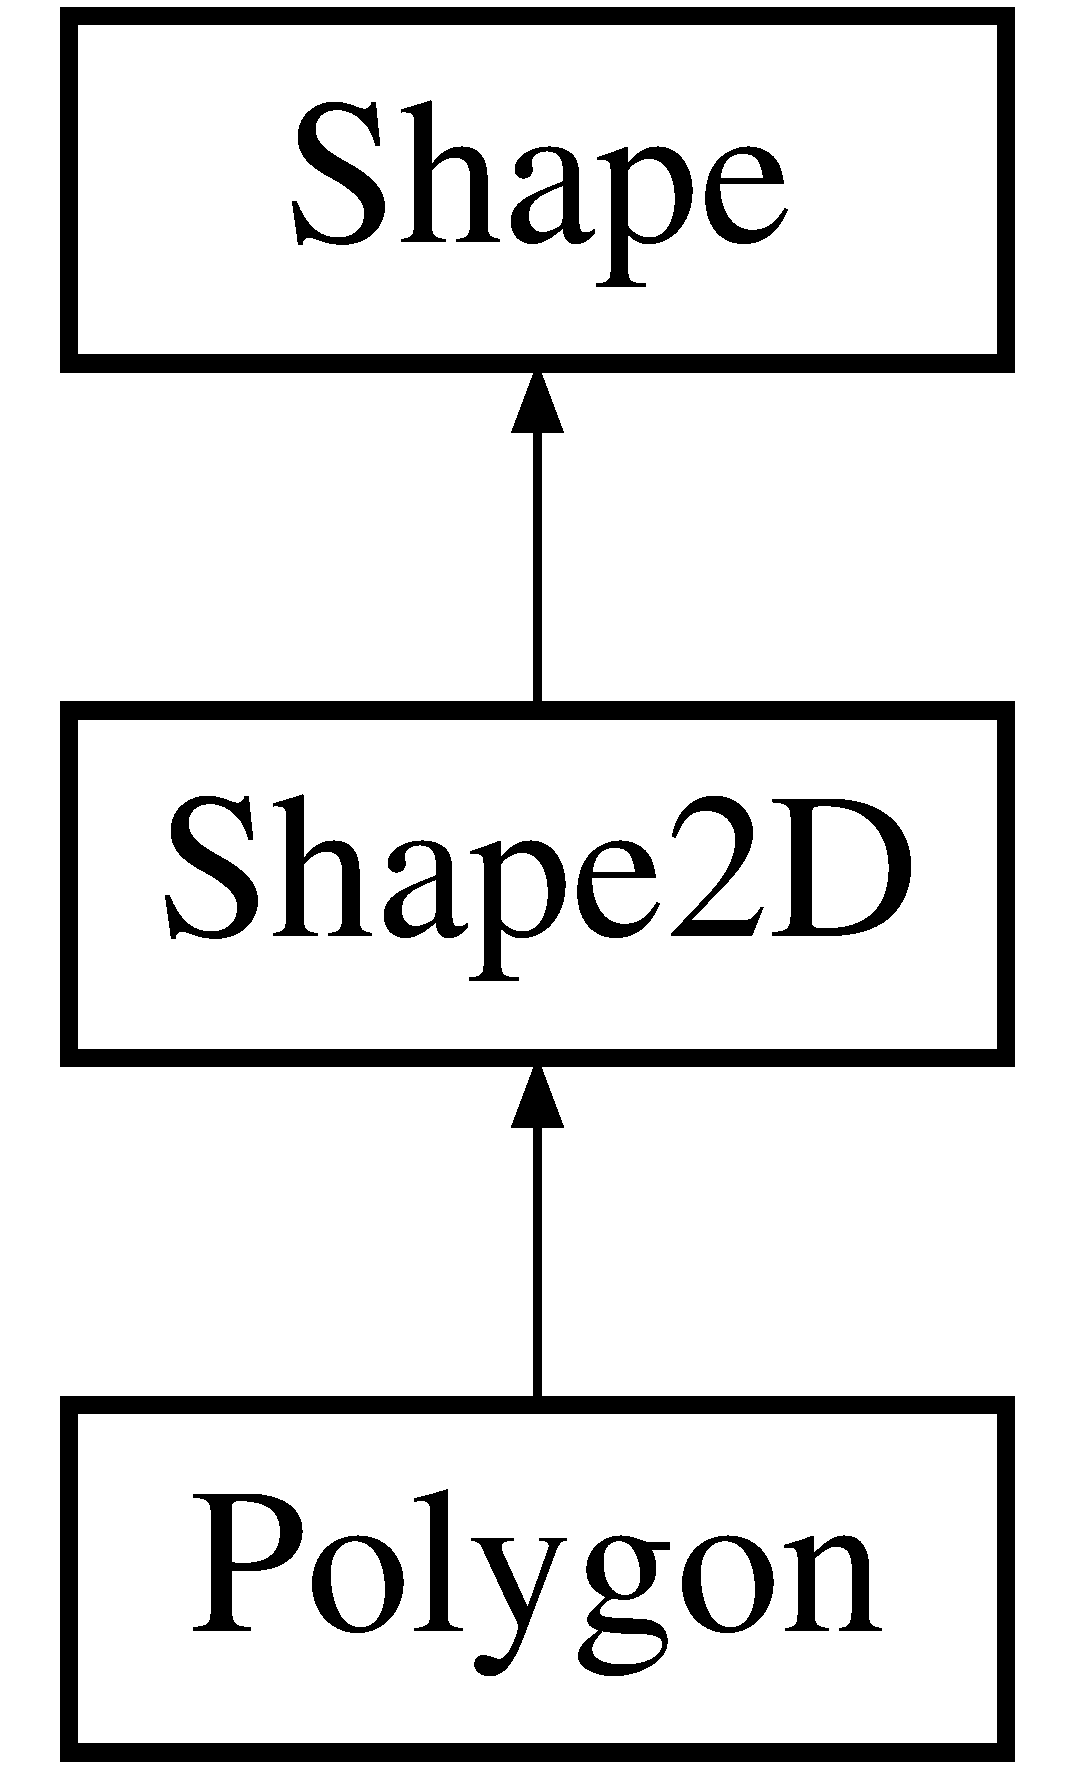
\includegraphics[height=3.000000cm]{classPolygon}
\end{center}
\end{figure}
\subsection*{Public Member Functions}
\begin{DoxyCompactItemize}
\item 
\hyperlink{classPolygon_a0a64a72fe34ecf25776b1bf0b33af9c9}{Polygon} (Q\-Paint\-Device $\ast$device, int x\-Id, Q\-Color x\-Pen\-Color, qreal x\-Pen\-Width, Qt\-::\-Pen\-Style x\-Pen\-Style, Qt\-::\-Pen\-Cap\-Style x\-Pen\-Cap\-Style, Qt\-::\-Pen\-Join\-Style x\-Pen\-Join\-Style, Q\-Color x\-Brush\-Color, Qt\-::\-Brush\-Style x\-Brush\-Style, const std\-::vector$<$ Q\-Point $>$ \&x\-Points)
\item 
\hypertarget{classPolygon_af39b679040579defec4a84276303c8f3}{\hyperlink{classPolygon}{Polygon} \& {\bfseries operator=} (const \hyperlink{classPolygon}{Polygon} \&)=delete}\label{classPolygon_af39b679040579defec4a84276303c8f3}

\item 
\hypertarget{classPolygon_a34540c02f39c27d1f140f47a92f58afb}{{\bfseries Polygon} (const \hyperlink{classPolygon}{Polygon} \&)=delete}\label{classPolygon_a34540c02f39c27d1f140f47a92f58afb}

\item 
\hyperlink{classPolygon_ace39c67107966db12e13a183f496c3b0}{$\sim$\-Polygon} ()
\item 
std\-::ostream \& \hyperlink{classPolygon_ae1d7135748131313fac844463013931e}{print} (std\-::ostream \&os) const 
\item 
void \hyperlink{classPolygon_a7161b79ad403b975423f73e0cd073343}{draw} (Q\-Paint\-Device $\ast$device)
\item 
void \hyperlink{classPolygon_a8972edcc7d98e79ac828905c4a52a272}{move} (Q\-Point \&new\-Upper\-Left)
\item 
void \hyperlink{classPolygon_a723d9ffbebe8964da953dcd52aafeec2}{update} (void)
\item 
double \hyperlink{classPolygon_a6756ed58b8fabebf1f02c89ea821fe78}{calc\-Perimeter} () const 
\item 
double \hyperlink{classPolygon_ac325f8f1af8622d7314b887b31603ba1}{calc\-Area} () const 
\end{DoxyCompactItemize}
\subsection*{Public Attributes}
\begin{DoxyCompactItemize}
\item 
vector$<$ Q\-Point $>$ \hyperlink{classPolygon_a2b9f4ab753cc0a4e8e844fac8c3d05a2}{points}
\end{DoxyCompactItemize}
\subsection*{Additional Inherited Members}


\subsection{Constructor \& Destructor Documentation}
\hypertarget{classPolygon_a0a64a72fe34ecf25776b1bf0b33af9c9}{\index{Polygon@{Polygon}!Polygon@{Polygon}}
\index{Polygon@{Polygon}!Polygon@{Polygon}}
\subsubsection[{Polygon}]{\setlength{\rightskip}{0pt plus 5cm}Polygon\-::\-Polygon (
\begin{DoxyParamCaption}
\item[{Q\-Paint\-Device $\ast$}]{device, }
\item[{int}]{x\-Id, }
\item[{Q\-Color}]{x\-Pen\-Color, }
\item[{qreal}]{x\-Pen\-Width, }
\item[{Qt\-::\-Pen\-Style}]{x\-Pen\-Style, }
\item[{Qt\-::\-Pen\-Cap\-Style}]{x\-Pen\-Cap\-Style, }
\item[{Qt\-::\-Pen\-Join\-Style}]{x\-Pen\-Join\-Style, }
\item[{Q\-Color}]{x\-Brush\-Color, }
\item[{Qt\-::\-Brush\-Style}]{x\-Brush\-Style, }
\item[{const std\-::vector$<$ Q\-Point $>$ \&}]{x\-Points}
\end{DoxyParamCaption}
)}}\label{classPolygon_a0a64a72fe34ecf25776b1bf0b33af9c9}
constructor -\/ create a Q\-T drawable polygon 2\-D

\begin{DoxyAuthor}{Author}
edt (5/14/18)
\end{DoxyAuthor}

\begin{DoxyParams}{Parameters}
{\em device} & \\
\hline
{\em x\-Id} & \\
\hline
{\em x\-Pen\-Color} & \\
\hline
{\em x\-Pen\-Width} & \\
\hline
{\em x\-Pen\-Style} & \\
\hline
{\em x\-Pen\-Cap\-Style} & \\
\hline
{\em x\-Pen\-Join\-Style} & \\
\hline
{\em x\-Brush\-Color} & \\
\hline
{\em x\-Brush\-Style} & \\
\hline
{\em x\-Points} & \\
\hline
\end{DoxyParams}
\hypertarget{classPolygon_ace39c67107966db12e13a183f496c3b0}{\index{Polygon@{Polygon}!$\sim$\-Polygon@{$\sim$\-Polygon}}
\index{$\sim$\-Polygon@{$\sim$\-Polygon}!Polygon@{Polygon}}
\subsubsection[{$\sim$\-Polygon}]{\setlength{\rightskip}{0pt plus 5cm}Polygon\-::$\sim$\-Polygon (
\begin{DoxyParamCaption}
{}
\end{DoxyParamCaption}
)}}\label{classPolygon_ace39c67107966db12e13a183f496c3b0}
Destructor -\/ simply free the object space

\begin{DoxyAuthor}{Author}
edt (5/13/18) 
\end{DoxyAuthor}


\subsection{Member Function Documentation}
\hypertarget{classPolygon_ac325f8f1af8622d7314b887b31603ba1}{\index{Polygon@{Polygon}!calc\-Area@{calc\-Area}}
\index{calc\-Area@{calc\-Area}!Polygon@{Polygon}}
\subsubsection[{calc\-Area}]{\setlength{\rightskip}{0pt plus 5cm}double Polygon\-::calc\-Area (
\begin{DoxyParamCaption}
\item[{void}]{}
\end{DoxyParamCaption}
) const\hspace{0.3cm}{\ttfamily [virtual]}}}\label{classPolygon_ac325f8f1af8622d7314b887b31603ba1}
calc\-Area -\/ determine area enclosed by object

\begin{DoxyAuthor}{Author}
edt (5/13/18)
\end{DoxyAuthor}
\begin{DoxyReturn}{Returns}
double 
\end{DoxyReturn}


Implements \hyperlink{classShape}{Shape}.

\hypertarget{classPolygon_a6756ed58b8fabebf1f02c89ea821fe78}{\index{Polygon@{Polygon}!calc\-Perimeter@{calc\-Perimeter}}
\index{calc\-Perimeter@{calc\-Perimeter}!Polygon@{Polygon}}
\subsubsection[{calc\-Perimeter}]{\setlength{\rightskip}{0pt plus 5cm}double Polygon\-::calc\-Perimeter (
\begin{DoxyParamCaption}
\item[{void}]{}
\end{DoxyParamCaption}
) const\hspace{0.3cm}{\ttfamily [virtual]}}}\label{classPolygon_a6756ed58b8fabebf1f02c89ea821fe78}
calc\-Perimeter -\/ determine object outline length

\begin{DoxyAuthor}{Author}
edt (5/13/18)
\end{DoxyAuthor}
\begin{DoxyReturn}{Returns}
double 
\end{DoxyReturn}


Implements \hyperlink{classShape}{Shape}.

\hypertarget{classPolygon_a7161b79ad403b975423f73e0cd073343}{\index{Polygon@{Polygon}!draw@{draw}}
\index{draw@{draw}!Polygon@{Polygon}}
\subsubsection[{draw}]{\setlength{\rightskip}{0pt plus 5cm}void Polygon\-::draw (
\begin{DoxyParamCaption}
\item[{Q\-Paint\-Device $\ast$}]{device}
\end{DoxyParamCaption}
)\hspace{0.3cm}{\ttfamily [virtual]}}}\label{classPolygon_a7161b79ad403b975423f73e0cd073343}
draw -\/ output object onto Q\-T canvas using Q\-Paint\-Device

\begin{DoxyAuthor}{Author}
edt (5/13/18)
\end{DoxyAuthor}

\begin{DoxyParams}{Parameters}
{\em device} & \\
\hline
\end{DoxyParams}


Implements \hyperlink{classShape}{Shape}.

\hypertarget{classPolygon_a8972edcc7d98e79ac828905c4a52a272}{\index{Polygon@{Polygon}!move@{move}}
\index{move@{move}!Polygon@{Polygon}}
\subsubsection[{move}]{\setlength{\rightskip}{0pt plus 5cm}void Polygon\-::move (
\begin{DoxyParamCaption}
\item[{Q\-Point \&}]{new\-Upper\-Left}
\end{DoxyParamCaption}
)\hspace{0.3cm}{\ttfamily [virtual]}}}\label{classPolygon_a8972edcc7d98e79ac828905c4a52a272}
move -\/ relocate polygon to new upper left coordinate

\begin{DoxyAuthor}{Author}
edt (5/13/18)
\end{DoxyAuthor}

\begin{DoxyParams}{Parameters}
{\em new\-Upper\-Left} & -\/ new location of upper left of enclosing rectangle \\
\hline
\end{DoxyParams}


Implements \hyperlink{classShape}{Shape}.

\hypertarget{classPolygon_ae1d7135748131313fac844463013931e}{\index{Polygon@{Polygon}!print@{print}}
\index{print@{print}!Polygon@{Polygon}}
\subsubsection[{print}]{\setlength{\rightskip}{0pt plus 5cm}std\-::ostream \& Polygon\-::print (
\begin{DoxyParamCaption}
\item[{std\-::ostream \&}]{os}
\end{DoxyParamCaption}
) const\hspace{0.3cm}{\ttfamily [virtual]}}}\label{classPolygon_ae1d7135748131313fac844463013931e}
print -\/ print limited information about derived instance for debugging

\begin{DoxyAuthor}{Author}
edt (5/13/18) 
\end{DoxyAuthor}


Implements \hyperlink{classShape2D_a6faf0b7950ea77a2ec6f29a31d65a624}{Shape2\-D}.

\hypertarget{classPolygon_a723d9ffbebe8964da953dcd52aafeec2}{\index{Polygon@{Polygon}!update@{update}}
\index{update@{update}!Polygon@{Polygon}}
\subsubsection[{update}]{\setlength{\rightskip}{0pt plus 5cm}void Polygon\-::update (
\begin{DoxyParamCaption}
\item[{void}]{}
\end{DoxyParamCaption}
)\hspace{0.3cm}{\ttfamily [virtual]}}}\label{classPolygon_a723d9ffbebe8964da953dcd52aafeec2}
update -\/ force redraw of object

\begin{DoxyAuthor}{Author}
edt (5/13/18)
\end{DoxyAuthor}

\begin{DoxyParams}{Parameters}
{\em void} & \\
\hline
\end{DoxyParams}


Implements \hyperlink{classShape}{Shape}.



\subsection{Member Data Documentation}
\hypertarget{classPolygon_a2b9f4ab753cc0a4e8e844fac8c3d05a2}{\index{Polygon@{Polygon}!points@{points}}
\index{points@{points}!Polygon@{Polygon}}
\subsubsection[{points}]{\setlength{\rightskip}{0pt plus 5cm}vector$<$Q\-Point$>$ Polygon\-::points}}\label{classPolygon_a2b9f4ab753cc0a4e8e844fac8c3d05a2}
points -\/ vector containing 3 or more points describing the vertices of the polygon 

The documentation for this class was generated from the following files\-:\begin{DoxyCompactItemize}
\item 
/home/edt/\-C\-S1\-C/\-Class\-Project/\-Main\-Window/polygon.\-h\item 
/home/edt/\-C\-S1\-C/\-Class\-Project/\-Main\-Window/polygon.\-cpp\end{DoxyCompactItemize}

\hypertarget{classPolyLine}{\section{Poly\-Line Class Reference}
\label{classPolyLine}\index{Poly\-Line@{Poly\-Line}}
}
Inheritance diagram for Poly\-Line\-:\begin{figure}[H]
\begin{center}
\leavevmode
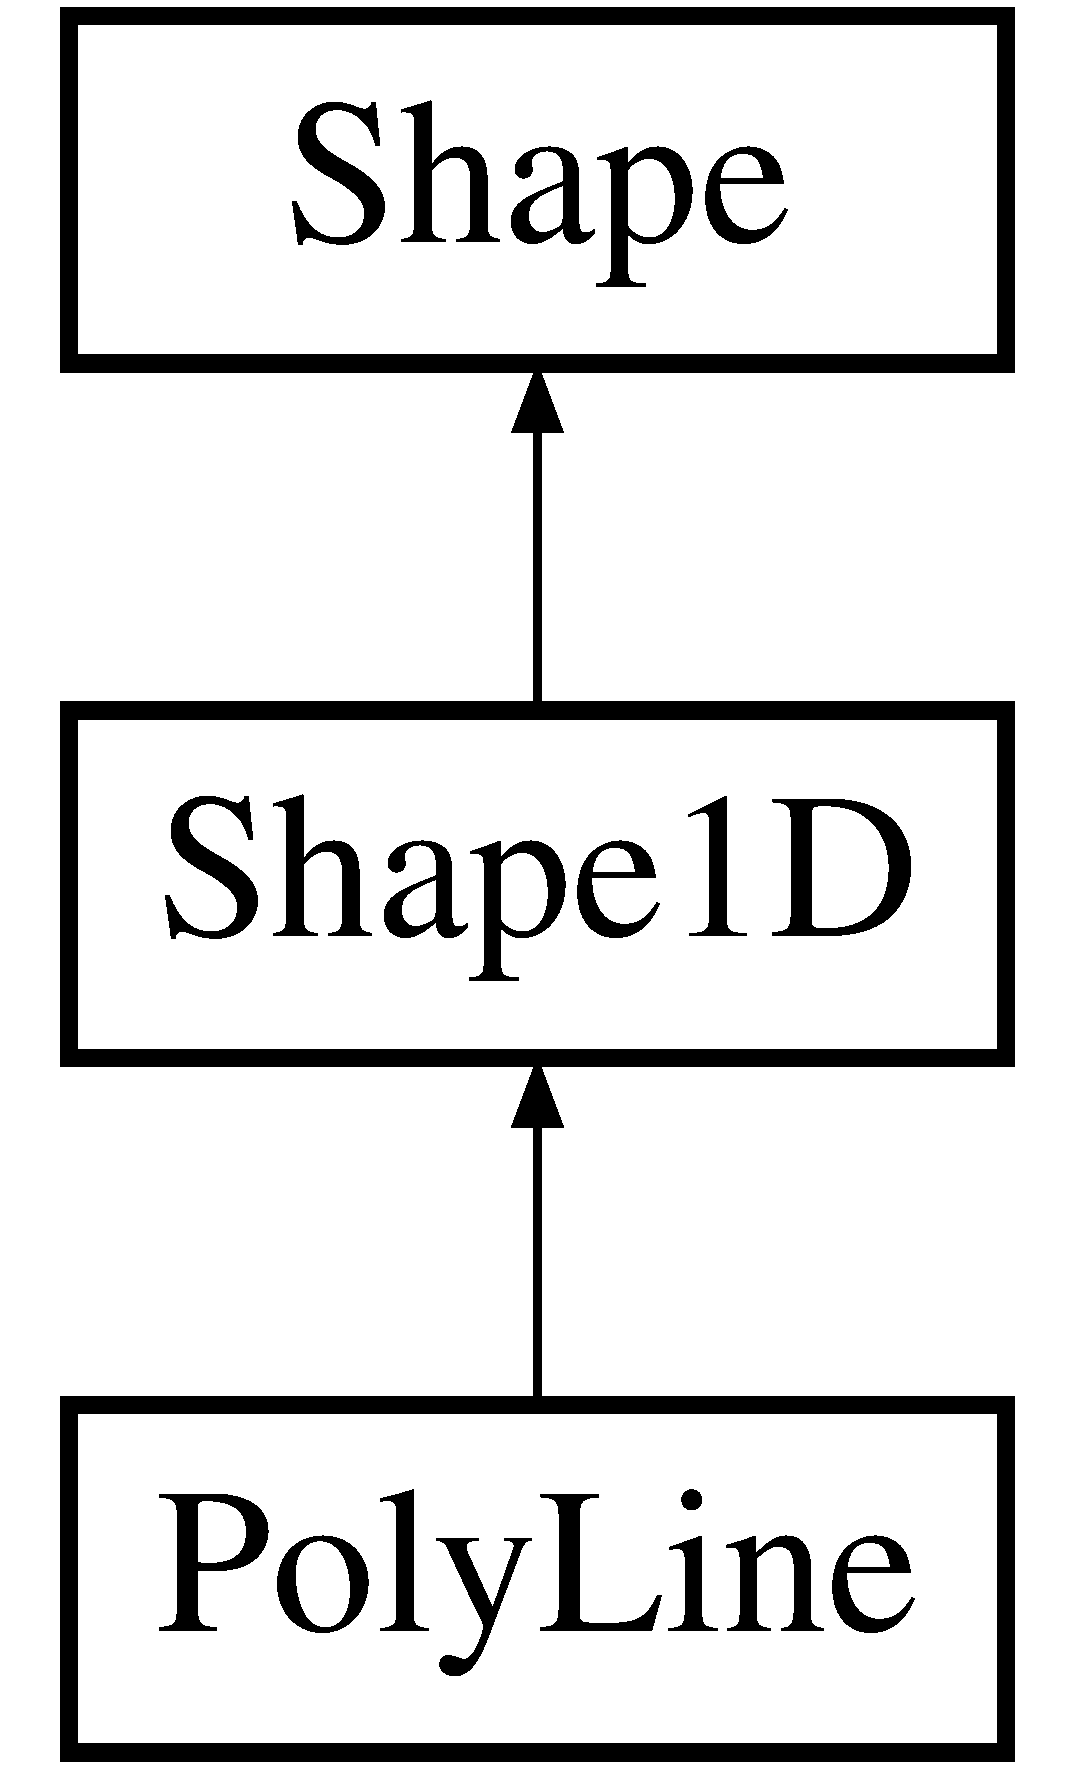
\includegraphics[height=3.000000cm]{classPolyLine}
\end{center}
\end{figure}
\subsection*{Public Member Functions}
\begin{DoxyCompactItemize}
\item 
\hyperlink{classPolyLine_a091b5af5ecbbfa2197a1b4b65274f00c}{Poly\-Line} (Q\-Paint\-Device $\ast$device, int x\-Id, Q\-Color x\-Pen\-Color, qreal x\-Pen\-Width, Qt\-::\-Pen\-Style x\-Pen\-Style, Qt\-::\-Pen\-Cap\-Style x\-Pen\-Cap\-Style, Qt\-::\-Pen\-Join\-Style x\-Pen\-Join\-Style, const std\-::vector$<$ Q\-Point $>$ \&x\-Points)
\item 
\hypertarget{classPolyLine_add038be40a45202389ee90e0d5eeb0fc}{\hyperlink{classPolyLine}{Poly\-Line} \& {\bfseries operator=} (const \hyperlink{classPolyLine}{Poly\-Line} \&)=delete}\label{classPolyLine_add038be40a45202389ee90e0d5eeb0fc}

\item 
\hypertarget{classPolyLine_a57f841f3dc099765f2d25aa07e577534}{{\bfseries Poly\-Line} (const \hyperlink{classPolyLine}{Poly\-Line} \&)=delete}\label{classPolyLine_a57f841f3dc099765f2d25aa07e577534}

\item 
\hyperlink{classPolyLine_ab086c534233b8b8c5eae909eb7a1c2dd}{$\sim$\-Poly\-Line} ()
\item 
std\-::ostream \& \hyperlink{classPolyLine_a716cc39a1e35f7538013760b0828aee6}{print} (std\-::ostream \&os) const 
\item 
void \hyperlink{classPolyLine_a6c4483740c346378276fbd70f007c3f5}{draw} (Q\-Paint\-Device $\ast$device)
\item 
void \hyperlink{classPolyLine_a6f9e35f1f05b2d50c741d09f4f653c4e}{move} (Q\-Point \&new\-Upper\-Left)
\item 
void \hyperlink{classPolyLine_a4d48598e631ad4e94a232e026f458555}{update} (void)
\item 
double \hyperlink{classPolyLine_add3cad6138ab4ccb76330360f208ab80}{calc\-Perimeter} () const 
\item 
double \hyperlink{classPolyLine_abed0b5ce3bab312119d7726c697f2fba}{calc\-Area} () const 
\end{DoxyCompactItemize}
\subsection*{Additional Inherited Members}


\subsection{Constructor \& Destructor Documentation}
\hypertarget{classPolyLine_a091b5af5ecbbfa2197a1b4b65274f00c}{\index{Poly\-Line@{Poly\-Line}!Poly\-Line@{Poly\-Line}}
\index{Poly\-Line@{Poly\-Line}!PolyLine@{Poly\-Line}}
\subsubsection[{Poly\-Line}]{\setlength{\rightskip}{0pt plus 5cm}Poly\-Line\-::\-Poly\-Line (
\begin{DoxyParamCaption}
\item[{Q\-Paint\-Device $\ast$}]{device, }
\item[{int}]{x\-Id, }
\item[{Q\-Color}]{x\-Pen\-Color, }
\item[{qreal}]{x\-Pen\-Width, }
\item[{Qt\-::\-Pen\-Style}]{x\-Pen\-Style, }
\item[{Qt\-::\-Pen\-Cap\-Style}]{x\-Pen\-Cap\-Style, }
\item[{Qt\-::\-Pen\-Join\-Style}]{x\-Pen\-Join\-Style, }
\item[{const std\-::vector$<$ Q\-Point $>$ \&}]{x\-Points}
\end{DoxyParamCaption}
)}}\label{classPolyLine_a091b5af5ecbbfa2197a1b4b65274f00c}
constructor -\/ create a Q\-T drawable line 1\-D

\begin{DoxyAuthor}{Author}
edt (5/14/18)
\end{DoxyAuthor}

\begin{DoxyParams}{Parameters}
{\em device} & -\/ Q\-Paint\-Device \\
\hline
{\em x\-Id} & -\/ shape I\-D \\
\hline
{\em x\-Pen\-Color} & \\
\hline
{\em x\-Pen\-Width} & \\
\hline
{\em x\-Pen\-Style} & \\
\hline
{\em x\-Pen\-Cap\-Style} & \\
\hline
{\em x\-Pen\-Join\-Style} & \\
\hline
{\em x\-Points} & \\
\hline
\end{DoxyParams}
\hypertarget{classPolyLine_ab086c534233b8b8c5eae909eb7a1c2dd}{\index{Poly\-Line@{Poly\-Line}!$\sim$\-Poly\-Line@{$\sim$\-Poly\-Line}}
\index{$\sim$\-Poly\-Line@{$\sim$\-Poly\-Line}!PolyLine@{Poly\-Line}}
\subsubsection[{$\sim$\-Poly\-Line}]{\setlength{\rightskip}{0pt plus 5cm}Poly\-Line\-::$\sim$\-Poly\-Line (
\begin{DoxyParamCaption}
{}
\end{DoxyParamCaption}
)}}\label{classPolyLine_ab086c534233b8b8c5eae909eb7a1c2dd}
Destructor -\/ simply free the object space

\begin{DoxyAuthor}{Author}
edt (5/13/18) 
\end{DoxyAuthor}


\subsection{Member Function Documentation}
\hypertarget{classPolyLine_abed0b5ce3bab312119d7726c697f2fba}{\index{Poly\-Line@{Poly\-Line}!calc\-Area@{calc\-Area}}
\index{calc\-Area@{calc\-Area}!PolyLine@{Poly\-Line}}
\subsubsection[{calc\-Area}]{\setlength{\rightskip}{0pt plus 5cm}double Poly\-Line\-::calc\-Area (
\begin{DoxyParamCaption}
\item[{void}]{}
\end{DoxyParamCaption}
) const\hspace{0.3cm}{\ttfamily [virtual]}}}\label{classPolyLine_abed0b5ce3bab312119d7726c697f2fba}
calc\-Area -\/ determine area enclosed by object

\begin{DoxyAuthor}{Author}
edt (5/13/18)
\end{DoxyAuthor}
\begin{DoxyReturn}{Returns}
double 
\end{DoxyReturn}


Implements \hyperlink{classShape}{Shape}.

\hypertarget{classPolyLine_add3cad6138ab4ccb76330360f208ab80}{\index{Poly\-Line@{Poly\-Line}!calc\-Perimeter@{calc\-Perimeter}}
\index{calc\-Perimeter@{calc\-Perimeter}!PolyLine@{Poly\-Line}}
\subsubsection[{calc\-Perimeter}]{\setlength{\rightskip}{0pt plus 5cm}double Poly\-Line\-::calc\-Perimeter (
\begin{DoxyParamCaption}
\item[{void}]{}
\end{DoxyParamCaption}
) const\hspace{0.3cm}{\ttfamily [virtual]}}}\label{classPolyLine_add3cad6138ab4ccb76330360f208ab80}
calc\-Perimeter -\/ determine object outline length

\begin{DoxyAuthor}{Author}
edt (5/13/18)
\end{DoxyAuthor}
\begin{DoxyReturn}{Returns}
double 
\end{DoxyReturn}


Implements \hyperlink{classShape}{Shape}.

\hypertarget{classPolyLine_a6c4483740c346378276fbd70f007c3f5}{\index{Poly\-Line@{Poly\-Line}!draw@{draw}}
\index{draw@{draw}!PolyLine@{Poly\-Line}}
\subsubsection[{draw}]{\setlength{\rightskip}{0pt plus 5cm}void Poly\-Line\-::draw (
\begin{DoxyParamCaption}
\item[{Q\-Paint\-Device $\ast$}]{device}
\end{DoxyParamCaption}
)\hspace{0.3cm}{\ttfamily [virtual]}}}\label{classPolyLine_a6c4483740c346378276fbd70f007c3f5}
draw -\/ output object onto Q\-T canvas using Q\-Paint\-Device

\begin{DoxyAuthor}{Author}
edt (5/13/18)
\end{DoxyAuthor}

\begin{DoxyParams}{Parameters}
{\em device} & \\
\hline
\end{DoxyParams}


Implements \hyperlink{classShape}{Shape}.

\hypertarget{classPolyLine_a6f9e35f1f05b2d50c741d09f4f653c4e}{\index{Poly\-Line@{Poly\-Line}!move@{move}}
\index{move@{move}!PolyLine@{Poly\-Line}}
\subsubsection[{move}]{\setlength{\rightskip}{0pt plus 5cm}void Poly\-Line\-::move (
\begin{DoxyParamCaption}
\item[{Q\-Point \&}]{new\-Upper\-Left}
\end{DoxyParamCaption}
)\hspace{0.3cm}{\ttfamily [virtual]}}}\label{classPolyLine_a6f9e35f1f05b2d50c741d09f4f653c4e}
move -\/ relocate line to new upper left coordinate

\begin{DoxyAuthor}{Author}
edt (5/13/18)
\end{DoxyAuthor}

\begin{DoxyParams}{Parameters}
{\em new\-Upper\-Left} & -\/ new location of upper left of enclosing rectangle \\
\hline
\end{DoxyParams}


Implements \hyperlink{classShape}{Shape}.

\hypertarget{classPolyLine_a716cc39a1e35f7538013760b0828aee6}{\index{Poly\-Line@{Poly\-Line}!print@{print}}
\index{print@{print}!PolyLine@{Poly\-Line}}
\subsubsection[{print}]{\setlength{\rightskip}{0pt plus 5cm}std\-::ostream \& Poly\-Line\-::print (
\begin{DoxyParamCaption}
\item[{std\-::ostream \&}]{os}
\end{DoxyParamCaption}
) const\hspace{0.3cm}{\ttfamily [virtual]}}}\label{classPolyLine_a716cc39a1e35f7538013760b0828aee6}
print -\/ print limited information about derived instance for debugging

\begin{DoxyAuthor}{Author}
edt (5/13/18)
\end{DoxyAuthor}

\begin{DoxyParams}{Parameters}
{\em os} & -\/ output stream\\
\hline
\end{DoxyParams}
\begin{DoxyReturn}{Returns}
std\-::ostream\& 
\end{DoxyReturn}


Implements \hyperlink{classShape1D_a20b9358df369b7b0fc4a1cdae5070836}{Shape1\-D}.

\hypertarget{classPolyLine_a4d48598e631ad4e94a232e026f458555}{\index{Poly\-Line@{Poly\-Line}!update@{update}}
\index{update@{update}!PolyLine@{Poly\-Line}}
\subsubsection[{update}]{\setlength{\rightskip}{0pt plus 5cm}void Poly\-Line\-::update (
\begin{DoxyParamCaption}
\item[{void}]{}
\end{DoxyParamCaption}
)\hspace{0.3cm}{\ttfamily [virtual]}}}\label{classPolyLine_a4d48598e631ad4e94a232e026f458555}
update -\/ force redraw of object

\begin{DoxyAuthor}{Author}
edt (5/13/18)
\end{DoxyAuthor}

\begin{DoxyParams}{Parameters}
{\em void} & \\
\hline
\end{DoxyParams}


Implements \hyperlink{classShape}{Shape}.



The documentation for this class was generated from the following files\-:\begin{DoxyCompactItemize}
\item 
/home/edt/\-C\-S1\-C/\-Class\-Project/\-Main\-Window/polyline.\-h\item 
/home/edt/\-C\-S1\-C/\-Class\-Project/\-Main\-Window/polyline.\-cpp\end{DoxyCompactItemize}

\hypertarget{classprivilege}{\section{privilege Class Reference}
\label{classprivilege}\index{privilege@{privilege}}
}


{\ttfamily \#include $<$privilege.\-h$>$}

Inheritance diagram for privilege\-:\begin{figure}[H]
\begin{center}
\leavevmode
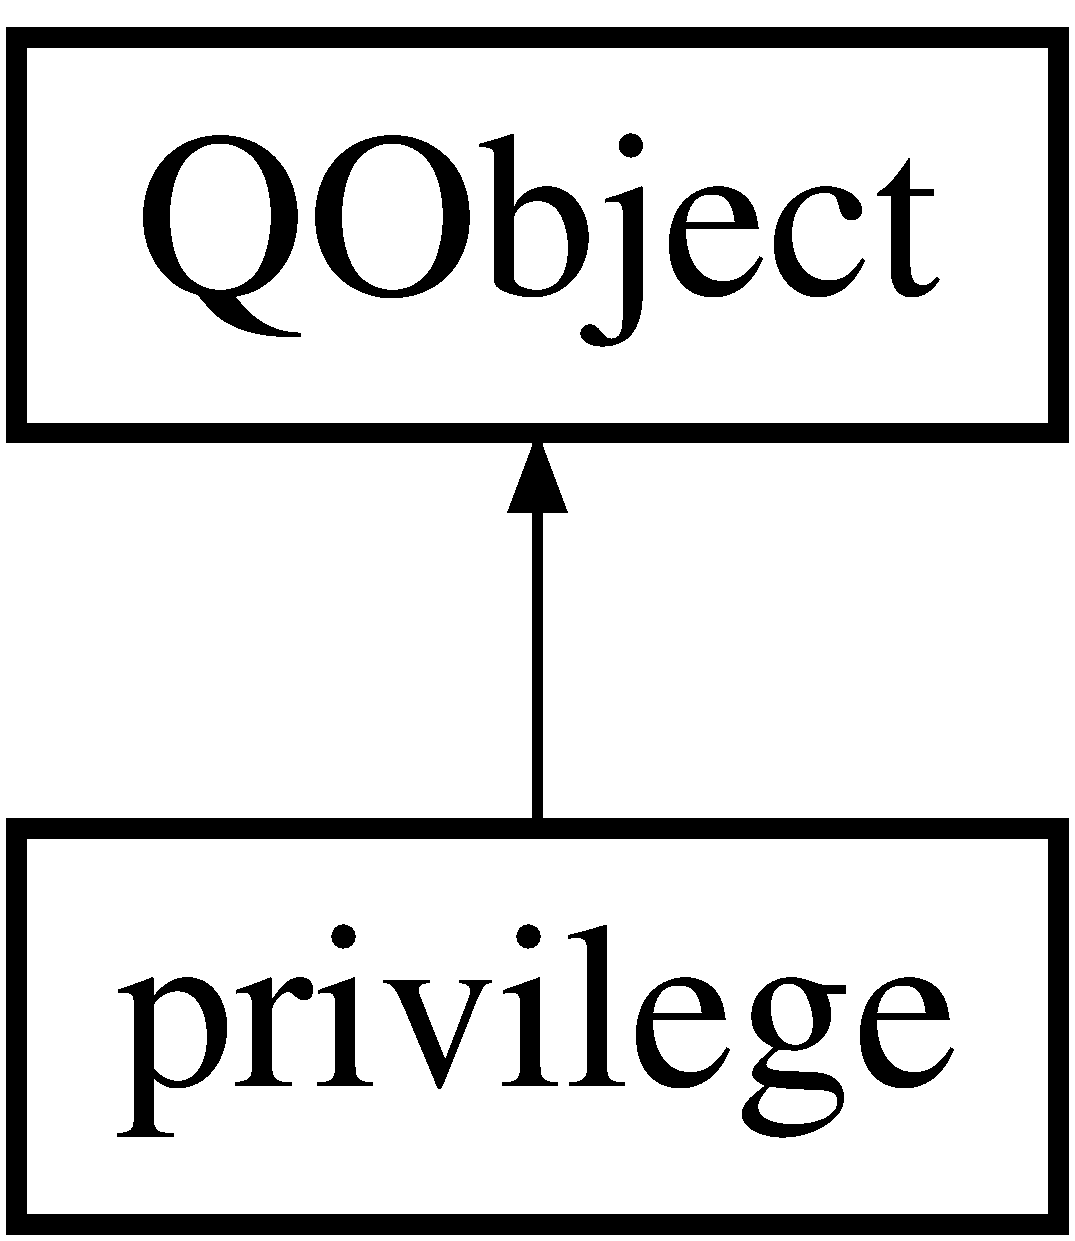
\includegraphics[height=2.000000cm]{classprivilege}
\end{center}
\end{figure}
\subsection*{Public Member Functions}
\begin{DoxyCompactItemize}
\item 
\hyperlink{classprivilege_a2b2b0d2232bc6868e6cfa9d519053ac9}{privilege} (int access=0)
\item 
bool \hyperlink{classprivilege_a3582979236988d258bbcc07fdd932d7f}{is\-Admin} () const 
\item 
bool \hyperlink{classprivilege_a640bdfa0e58d71ba1945bbd12fab1d76}{is\-User} () const 
\item 
int \hyperlink{classprivilege_a3924d6b685150666db220ea6c4f3b895}{get\-Access} () const 
\item 
void \hyperlink{classprivilege_a9fbdc8331a8c340ae8e841c01967fb15}{set\-Access} (int acc)
\end{DoxyCompactItemize}


\subsection{Detailed Description}
privilege class -\/ manage user privileges

\begin{DoxyAuthor}{Author}
richard (5/14/18) 
\end{DoxyAuthor}


\subsection{Constructor \& Destructor Documentation}
\hypertarget{classprivilege_a2b2b0d2232bc6868e6cfa9d519053ac9}{\index{privilege@{privilege}!privilege@{privilege}}
\index{privilege@{privilege}!privilege@{privilege}}
\subsubsection[{privilege}]{\setlength{\rightskip}{0pt plus 5cm}privilege\-::privilege (
\begin{DoxyParamCaption}
\item[{int}]{access = {\ttfamily 0}}
\end{DoxyParamCaption}
)\hspace{0.3cm}{\ttfamily [inline]}}}\label{classprivilege_a2b2b0d2232bc6868e6cfa9d519053ac9}
constructor -\/ create instance for user

\begin{DoxyAuthor}{Author}
richard (5/14/18)
\end{DoxyAuthor}

\begin{DoxyParams}{Parameters}
{\em access} & -\/ allowed access level \\
\hline
\end{DoxyParams}


\subsection{Member Function Documentation}
\hypertarget{classprivilege_a3924d6b685150666db220ea6c4f3b895}{\index{privilege@{privilege}!get\-Access@{get\-Access}}
\index{get\-Access@{get\-Access}!privilege@{privilege}}
\subsubsection[{get\-Access}]{\setlength{\rightskip}{0pt plus 5cm}int privilege\-::get\-Access (
\begin{DoxyParamCaption}
{}
\end{DoxyParamCaption}
) const\hspace{0.3cm}{\ttfamily [inline]}}}\label{classprivilege_a3924d6b685150666db220ea6c4f3b895}
get\-Access -\/ fetch access level

\begin{DoxyAuthor}{Author}
richard (5/14/18)
\end{DoxyAuthor}
\begin{DoxyReturn}{Returns}
int -\/ access level 
\end{DoxyReturn}
\hypertarget{classprivilege_a3582979236988d258bbcc07fdd932d7f}{\index{privilege@{privilege}!is\-Admin@{is\-Admin}}
\index{is\-Admin@{is\-Admin}!privilege@{privilege}}
\subsubsection[{is\-Admin}]{\setlength{\rightskip}{0pt plus 5cm}bool privilege\-::is\-Admin (
\begin{DoxyParamCaption}
{}
\end{DoxyParamCaption}
) const\hspace{0.3cm}{\ttfamily [inline]}}}\label{classprivilege_a3582979236988d258bbcc07fdd932d7f}
is\-Admin -\/ determine user level

\begin{DoxyAuthor}{Author}
richard (5/14/18)
\end{DoxyAuthor}
\begin{DoxyReturn}{Returns}
bool -\/ true if admin user 
\end{DoxyReturn}
\hypertarget{classprivilege_a640bdfa0e58d71ba1945bbd12fab1d76}{\index{privilege@{privilege}!is\-User@{is\-User}}
\index{is\-User@{is\-User}!privilege@{privilege}}
\subsubsection[{is\-User}]{\setlength{\rightskip}{0pt plus 5cm}bool privilege\-::is\-User (
\begin{DoxyParamCaption}
{}
\end{DoxyParamCaption}
) const\hspace{0.3cm}{\ttfamily [inline]}}}\label{classprivilege_a640bdfa0e58d71ba1945bbd12fab1d76}
is\-User -\/ detemine user level

\begin{DoxyAuthor}{Author}
richard (5/14/18)
\end{DoxyAuthor}
\begin{DoxyReturn}{Returns}
bool -\/ true if regular user 
\end{DoxyReturn}
\hypertarget{classprivilege_a9fbdc8331a8c340ae8e841c01967fb15}{\index{privilege@{privilege}!set\-Access@{set\-Access}}
\index{set\-Access@{set\-Access}!privilege@{privilege}}
\subsubsection[{set\-Access}]{\setlength{\rightskip}{0pt plus 5cm}void privilege\-::set\-Access (
\begin{DoxyParamCaption}
\item[{int}]{acc}
\end{DoxyParamCaption}
)\hspace{0.3cm}{\ttfamily [inline]}}}\label{classprivilege_a9fbdc8331a8c340ae8e841c01967fb15}
set\-Access -\/ store access level

\begin{DoxyAuthor}{Author}
richard (5/14/18)
\end{DoxyAuthor}

\begin{DoxyParams}{Parameters}
{\em acc} & -\/ access level to store \\
\hline
\end{DoxyParams}


The documentation for this class was generated from the following file\-:\begin{DoxyCompactItemize}
\item 
/home/edt/\-C\-S1\-C/\-Class\-Project/\-Main\-Window/privilege.\-h\end{DoxyCompactItemize}

\hypertarget{classRectangle}{\section{Rectangle Class Reference}
\label{classRectangle}\index{Rectangle@{Rectangle}}
}
Inheritance diagram for Rectangle\-:\begin{figure}[H]
\begin{center}
\leavevmode
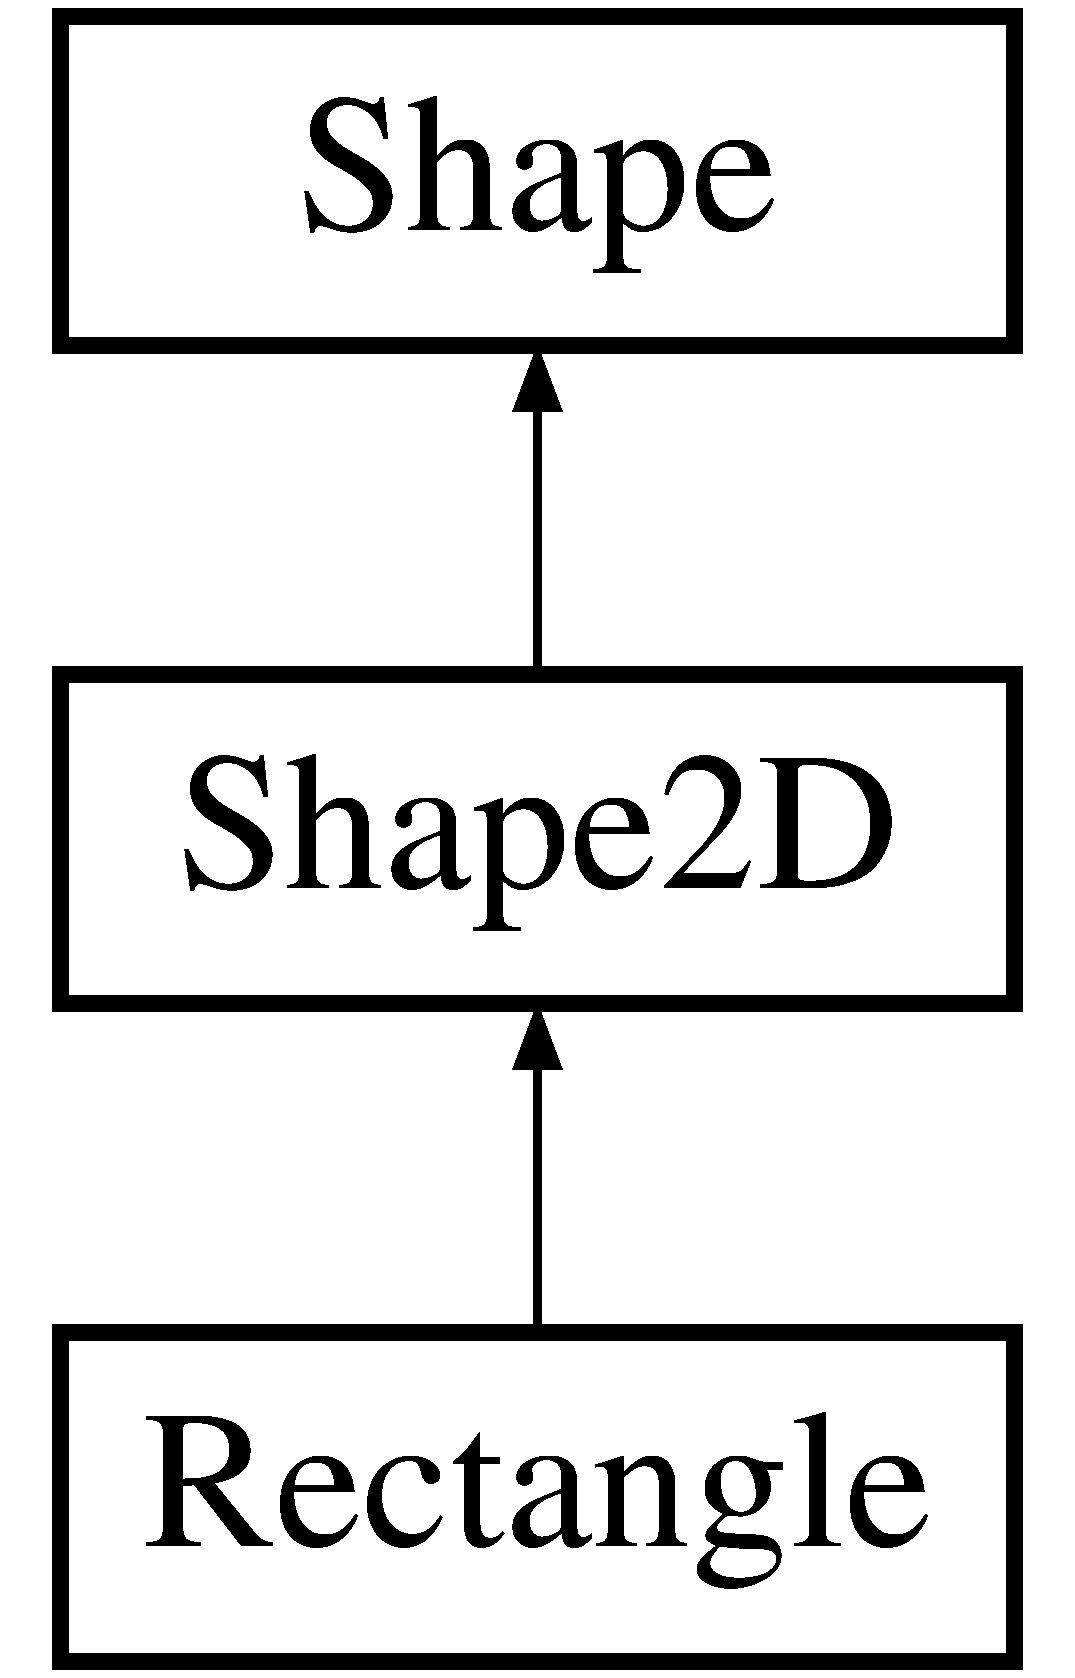
\includegraphics[height=3.000000cm]{classRectangle}
\end{center}
\end{figure}
\subsection*{Public Member Functions}
\begin{DoxyCompactItemize}
\item 
\hyperlink{classRectangle_a6e0872acf1be9c941846e9b2548e04af}{Rectangle} (Q\-Paint\-Device $\ast$device, int x\-Id, Q\-Color x\-Pen\-Color, qreal x\-Pen\-Width, Qt\-::\-Pen\-Style x\-Pen\-Style, Qt\-::\-Pen\-Cap\-Style x\-Pen\-Cap\-Style, Qt\-::\-Pen\-Join\-Style x\-Pen\-Join\-Style, Q\-Color x\-Brush\-Color, Qt\-::\-Brush\-Style x\-Brush\-Style, int x\-Top\-Left\-X, int x\-Top\-Left\-Y, int x\-Width, int x\-Height)
\item 
\hypertarget{classRectangle_a493870acad785dd377201c06c28003e4}{\hyperlink{classRectangle}{Rectangle} \& {\bfseries operator=} (const \hyperlink{classRectangle}{Rectangle} \&)=delete}\label{classRectangle_a493870acad785dd377201c06c28003e4}

\item 
\hypertarget{classRectangle_aee647897178612d4e18b9496bed0b58d}{{\bfseries Rectangle} (const \hyperlink{classRectangle}{Rectangle} \&)=delete}\label{classRectangle_aee647897178612d4e18b9496bed0b58d}

\item 
\hyperlink{classRectangle_a494c076b13aadf26efdce07d23c61ddd}{$\sim$\-Rectangle} ()
\item 
std\-::ostream \& \hyperlink{classRectangle_a06528cd92243f56f5eca551c5d637657}{print} (std\-::ostream \&os) const 
\item 
void \hyperlink{classRectangle_acd4e738aca00c23c0f1b15d77fec5dd8}{draw} (Q\-Paint\-Device $\ast$device)
\item 
void \hyperlink{classRectangle_a1fbeb44ec8b9400a5bfa7c0124fb29ee}{move} (Q\-Point \&new\-Upper\-Left)
\item 
void \hyperlink{classRectangle_a1679d95f9c3f0794a9fc54ca26509b6f}{update} (void)
\item 
double \hyperlink{classRectangle_af839a919dea3752e1d3dfad0282d19a1}{calc\-Perimeter} () const 
\item 
double \hyperlink{classRectangle_afa0bed5922c9517f5f771ed821f8623b}{calc\-Area} () const 
\end{DoxyCompactItemize}
\subsection*{Additional Inherited Members}


\subsection{Constructor \& Destructor Documentation}
\hypertarget{classRectangle_a6e0872acf1be9c941846e9b2548e04af}{\index{Rectangle@{Rectangle}!Rectangle@{Rectangle}}
\index{Rectangle@{Rectangle}!Rectangle@{Rectangle}}
\subsubsection[{Rectangle}]{\setlength{\rightskip}{0pt plus 5cm}Rectangle\-::\-Rectangle (
\begin{DoxyParamCaption}
\item[{Q\-Paint\-Device $\ast$}]{device, }
\item[{int}]{x\-Id, }
\item[{Q\-Color}]{x\-Pen\-Color, }
\item[{qreal}]{x\-Pen\-Width, }
\item[{Qt\-::\-Pen\-Style}]{x\-Pen\-Style, }
\item[{Qt\-::\-Pen\-Cap\-Style}]{x\-Pen\-Cap\-Style, }
\item[{Qt\-::\-Pen\-Join\-Style}]{x\-Pen\-Join\-Style, }
\item[{Q\-Color}]{x\-Brush\-Color, }
\item[{Qt\-::\-Brush\-Style}]{x\-Brush\-Style, }
\item[{int}]{x\-Top\-Left\-X, }
\item[{int}]{x\-Top\-Left\-Y, }
\item[{int}]{x\-Width, }
\item[{int}]{x\-Height}
\end{DoxyParamCaption}
)}}\label{classRectangle_a6e0872acf1be9c941846e9b2548e04af}
Constructor -\/ create a Q\-T drawable rectangle 2\-D

\begin{DoxyAuthor}{Author}
edt (5/14/18)
\end{DoxyAuthor}

\begin{DoxyParams}{Parameters}
{\em device} & -\/ Q\-Paint\-Device \\
\hline
{\em x\-Id} & -\/ shape I\-D \\
\hline
{\em x\-Pen\-Color} & \\
\hline
{\em x\-Pen\-Width} & \\
\hline
{\em x\-Pen\-Style} & \\
\hline
{\em x\-Pen\-Cap\-Style} & \\
\hline
{\em x\-Pen\-Join\-Style} & \\
\hline
{\em x\-Brush\-Color} & \\
\hline
{\em x\-Brush\-Style} & \\
\hline
{\em x\-Top\-Left\-X} & \\
\hline
{\em x\-Top\-Left\-Y} & \\
\hline
{\em x\-Width} & \\
\hline
{\em x\-Height} & \\
\hline
\end{DoxyParams}
\hypertarget{classRectangle_a494c076b13aadf26efdce07d23c61ddd}{\index{Rectangle@{Rectangle}!$\sim$\-Rectangle@{$\sim$\-Rectangle}}
\index{$\sim$\-Rectangle@{$\sim$\-Rectangle}!Rectangle@{Rectangle}}
\subsubsection[{$\sim$\-Rectangle}]{\setlength{\rightskip}{0pt plus 5cm}Rectangle\-::$\sim$\-Rectangle (
\begin{DoxyParamCaption}
{}
\end{DoxyParamCaption}
)}}\label{classRectangle_a494c076b13aadf26efdce07d23c61ddd}
Destructor -\/ simply free the object space

\begin{DoxyAuthor}{Author}
edt (5/13/18) 
\end{DoxyAuthor}


\subsection{Member Function Documentation}
\hypertarget{classRectangle_afa0bed5922c9517f5f771ed821f8623b}{\index{Rectangle@{Rectangle}!calc\-Area@{calc\-Area}}
\index{calc\-Area@{calc\-Area}!Rectangle@{Rectangle}}
\subsubsection[{calc\-Area}]{\setlength{\rightskip}{0pt plus 5cm}double Rectangle\-::calc\-Area (
\begin{DoxyParamCaption}
\item[{void}]{}
\end{DoxyParamCaption}
) const\hspace{0.3cm}{\ttfamily [virtual]}}}\label{classRectangle_afa0bed5922c9517f5f771ed821f8623b}
calc\-Area -\/ determine area enclosed by object

\begin{DoxyAuthor}{Author}
edt (5/13/18)
\end{DoxyAuthor}
\begin{DoxyReturn}{Returns}
double 
\end{DoxyReturn}


Implements \hyperlink{classShape}{Shape}.

\hypertarget{classRectangle_af839a919dea3752e1d3dfad0282d19a1}{\index{Rectangle@{Rectangle}!calc\-Perimeter@{calc\-Perimeter}}
\index{calc\-Perimeter@{calc\-Perimeter}!Rectangle@{Rectangle}}
\subsubsection[{calc\-Perimeter}]{\setlength{\rightskip}{0pt plus 5cm}double Rectangle\-::calc\-Perimeter (
\begin{DoxyParamCaption}
\item[{void}]{}
\end{DoxyParamCaption}
) const\hspace{0.3cm}{\ttfamily [virtual]}}}\label{classRectangle_af839a919dea3752e1d3dfad0282d19a1}
calc\-Perimeter -\/ determine object outline length

\begin{DoxyAuthor}{Author}
edt (5/13/18)
\end{DoxyAuthor}
\begin{DoxyReturn}{Returns}
double 
\end{DoxyReturn}


Implements \hyperlink{classShape}{Shape}.

\hypertarget{classRectangle_acd4e738aca00c23c0f1b15d77fec5dd8}{\index{Rectangle@{Rectangle}!draw@{draw}}
\index{draw@{draw}!Rectangle@{Rectangle}}
\subsubsection[{draw}]{\setlength{\rightskip}{0pt plus 5cm}void Rectangle\-::draw (
\begin{DoxyParamCaption}
\item[{Q\-Paint\-Device $\ast$}]{device}
\end{DoxyParamCaption}
)\hspace{0.3cm}{\ttfamily [virtual]}}}\label{classRectangle_acd4e738aca00c23c0f1b15d77fec5dd8}
draw -\/ output object onto Q\-T canvas using Q\-Paint\-Device

\begin{DoxyAuthor}{Author}
edt (5/13/18)
\end{DoxyAuthor}

\begin{DoxyParams}{Parameters}
{\em device} & \\
\hline
\end{DoxyParams}


Implements \hyperlink{classShape}{Shape}.

\hypertarget{classRectangle_a1fbeb44ec8b9400a5bfa7c0124fb29ee}{\index{Rectangle@{Rectangle}!move@{move}}
\index{move@{move}!Rectangle@{Rectangle}}
\subsubsection[{move}]{\setlength{\rightskip}{0pt plus 5cm}void Rectangle\-::move (
\begin{DoxyParamCaption}
\item[{Q\-Point \&}]{new\-Upper\-Left}
\end{DoxyParamCaption}
)\hspace{0.3cm}{\ttfamily [virtual]}}}\label{classRectangle_a1fbeb44ec8b9400a5bfa7c0124fb29ee}
move -\/ relocate rectangle to new upper left coordinate

\begin{DoxyAuthor}{Author}
edt (5/13/18)
\end{DoxyAuthor}

\begin{DoxyParams}{Parameters}
{\em new\-Upper\-Left} & -\/ new location of upper left of enclosing rectangle \\
\hline
\end{DoxyParams}


Implements \hyperlink{classShape}{Shape}.

\hypertarget{classRectangle_a06528cd92243f56f5eca551c5d637657}{\index{Rectangle@{Rectangle}!print@{print}}
\index{print@{print}!Rectangle@{Rectangle}}
\subsubsection[{print}]{\setlength{\rightskip}{0pt plus 5cm}std\-::ostream \& Rectangle\-::print (
\begin{DoxyParamCaption}
\item[{std\-::ostream \&}]{os}
\end{DoxyParamCaption}
) const\hspace{0.3cm}{\ttfamily [virtual]}}}\label{classRectangle_a06528cd92243f56f5eca551c5d637657}
print -\/ print limited information about derived instance for debugging

\begin{DoxyAuthor}{Author}
edt (5/13/18)
\end{DoxyAuthor}

\begin{DoxyParams}{Parameters}
{\em os} & -\/ output stream\\
\hline
\end{DoxyParams}
\begin{DoxyReturn}{Returns}
std\-::ostream\& 
\end{DoxyReturn}


Implements \hyperlink{classShape2D_a6faf0b7950ea77a2ec6f29a31d65a624}{Shape2\-D}.

\hypertarget{classRectangle_a1679d95f9c3f0794a9fc54ca26509b6f}{\index{Rectangle@{Rectangle}!update@{update}}
\index{update@{update}!Rectangle@{Rectangle}}
\subsubsection[{update}]{\setlength{\rightskip}{0pt plus 5cm}void Rectangle\-::update (
\begin{DoxyParamCaption}
\item[{void}]{}
\end{DoxyParamCaption}
)\hspace{0.3cm}{\ttfamily [virtual]}}}\label{classRectangle_a1679d95f9c3f0794a9fc54ca26509b6f}
update -\/ force redraw of object

\begin{DoxyAuthor}{Author}
edt (5/13/18)
\end{DoxyAuthor}

\begin{DoxyParams}{Parameters}
{\em void} & \\
\hline
\end{DoxyParams}


Implements \hyperlink{classShape}{Shape}.



The documentation for this class was generated from the following files\-:\begin{DoxyCompactItemize}
\item 
/home/edt/\-C\-S1\-C/\-Class\-Project/\-Main\-Window/rectangle.\-h\item 
/home/edt/\-C\-S1\-C/\-Class\-Project/\-Main\-Window/rectangle.\-cpp\end{DoxyCompactItemize}

\hypertarget{classrenderArea}{\section{render\-Area Class Reference}
\label{classrenderArea}\index{render\-Area@{render\-Area}}
}
Inheritance diagram for render\-Area\-:\begin{figure}[H]
\begin{center}
\leavevmode
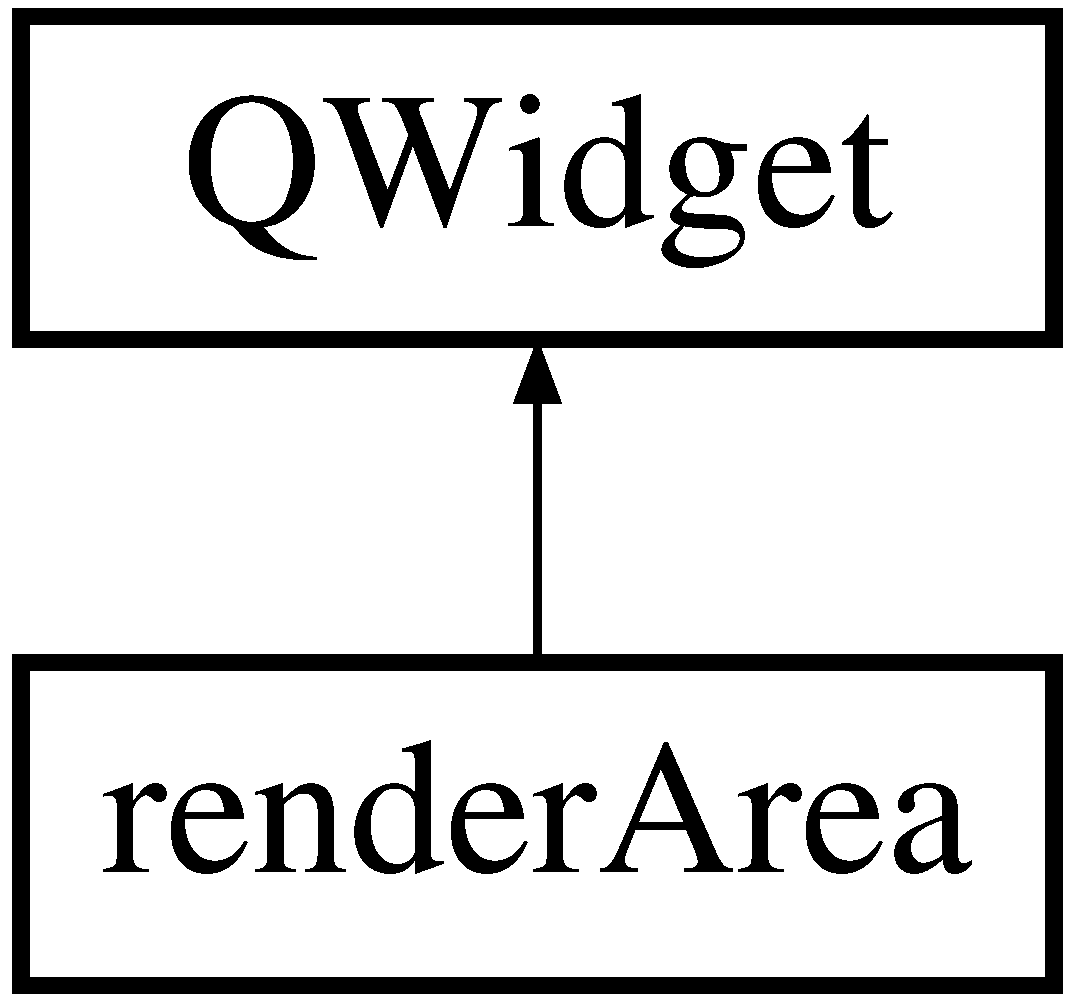
\includegraphics[height=2.000000cm]{classrenderArea}
\end{center}
\end{figure}


The documentation for this class was generated from the following files\-:\begin{DoxyCompactItemize}
\item 
/home/edt/\-C\-S1\-C/\-Class\-Project/\-Main\-Window/renderarea.\-h\item 
/home/edt/\-C\-S1\-C/\-Class\-Project/\-Main\-Window/renderarea.\-cpp\end{DoxyCompactItemize}

\hypertarget{classreports}{\section{reports Class Reference}
\label{classreports}\index{reports@{reports}}
}
Inheritance diagram for reports\-:\begin{figure}[H]
\begin{center}
\leavevmode
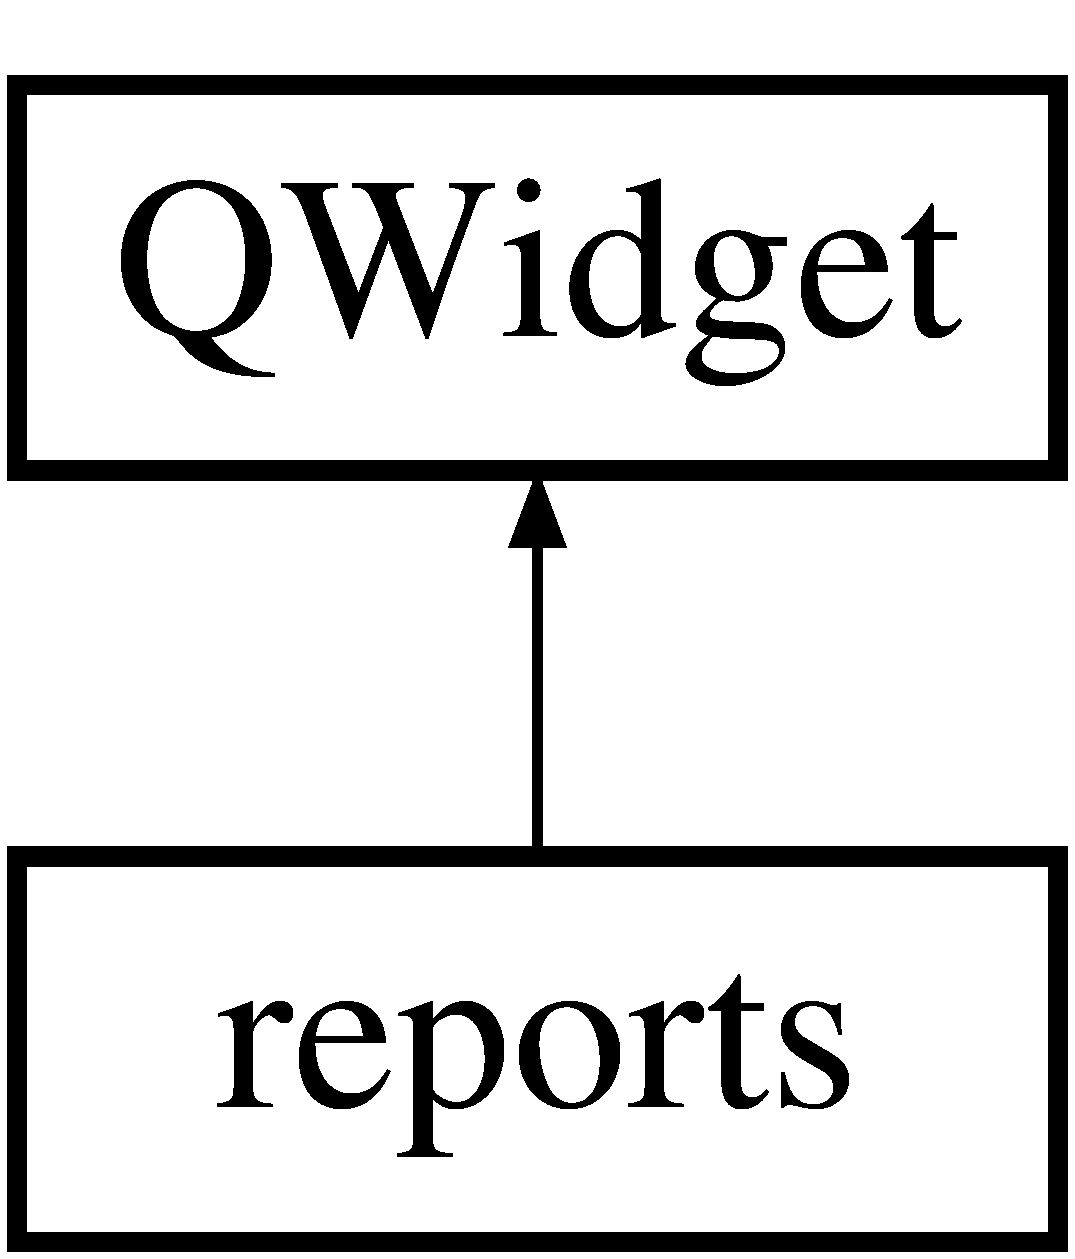
\includegraphics[height=2.000000cm]{classreports}
\end{center}
\end{figure}
\subsection*{Public Member Functions}
\begin{DoxyCompactItemize}
\item 
\hypertarget{classreports_aa1efd01d6a2a715cad88423fac7380f6}{{\bfseries reports} (Q\-Widget $\ast$parent=0)}\label{classreports_aa1efd01d6a2a715cad88423fac7380f6}

\end{DoxyCompactItemize}


The documentation for this class was generated from the following files\-:\begin{DoxyCompactItemize}
\item 
/home/edt/\-C\-S1\-C/\-Class\-Project/\-Main\-Window/reports.\-h\item 
/home/edt/\-C\-S1\-C/\-Class\-Project/\-Main\-Window/reports.\-cpp\end{DoxyCompactItemize}

\hypertarget{classShape}{\section{Shape Class Reference}
\label{classShape}\index{Shape@{Shape}}
}
Inheritance diagram for Shape\-:\begin{figure}[H]
\begin{center}
\leavevmode
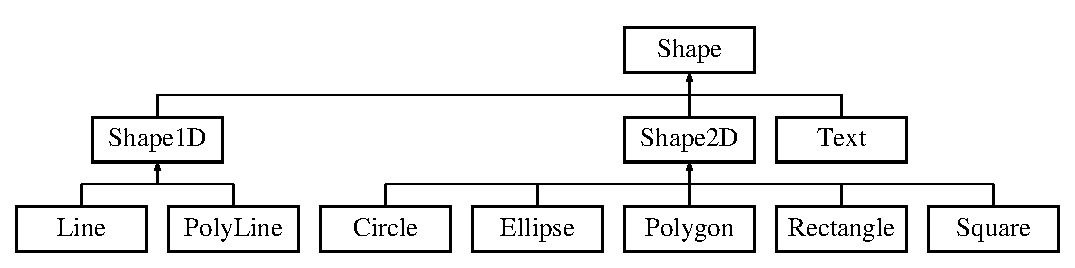
\includegraphics[height=3.000000cm]{classShape}
\end{center}
\end{figure}
\subsection*{Public Types}
\begin{DoxyCompactItemize}
\item 
enum \hyperlink{classShape_aaac58aa2f6760d0f06ec1710d5123e9b}{shape\-Type} \{ \\*
{\bfseries Line}, 
{\bfseries Polyline}, 
{\bfseries Polygon}, 
{\bfseries Rectangle}, 
\\*
{\bfseries Square}, 
{\bfseries Ellipse}, 
{\bfseries Circle}, 
{\bfseries Text}
 \}
\end{DoxyCompactItemize}
\subsection*{Public Member Functions}
\begin{DoxyCompactItemize}
\item 
\hypertarget{classShape_a299b81fd56576b079f942a6a2c2f64e7}{{\bfseries Shape} (Q\-Paint\-Device $\ast$p\-Device, int x\-Id, \hyperlink{classShape_aaac58aa2f6760d0f06ec1710d5123e9b}{shape\-Type} s)}\label{classShape_a299b81fd56576b079f942a6a2c2f64e7}

\item 
\hypertarget{classShape_a9b9942917d6e6c359a8751156ed52423}{\hyperlink{classShape}{Shape} \& {\bfseries operator=} (const \hyperlink{classShape}{Shape} \&)=delete}\label{classShape_a9b9942917d6e6c359a8751156ed52423}

\item 
\hypertarget{classShape_a44d91c7621d4d7af60fe3320a2e07279}{{\bfseries Shape} (const \hyperlink{classShape}{Shape} \&)=delete}\label{classShape_a44d91c7621d4d7af60fe3320a2e07279}

\item 
int \hyperlink{classShape_a8783318515d368f9ba7b8f73a343e59b}{get\-Id} () const 
\item 
\hyperlink{classShape_aaac58aa2f6760d0f06ec1710d5123e9b}{shape\-Type} \hyperlink{classShape_a76eade96838eac557423a4ca8c0d9aef}{get\-Shape\-Type} () const 
\item 
\hypertarget{classShape_a0605dd98087b8566090acd67dc71eaa9}{virtual void {\bfseries draw} (Q\-Paint\-Device $\ast$p\-Device)=0}\label{classShape_a0605dd98087b8566090acd67dc71eaa9}

\item 
\hypertarget{classShape_a7314802497e54a2e3394eb5c9eacf06c}{virtual void {\bfseries move} (Q\-Point \&new\-Upper\-Left)=0}\label{classShape_a7314802497e54a2e3394eb5c9eacf06c}

\item 
\hypertarget{classShape_ad17bd222fddba504d2b995dede3ce1ba}{virtual void {\bfseries update} (void)=0}\label{classShape_ad17bd222fddba504d2b995dede3ce1ba}

\item 
\hypertarget{classShape_a3167ca12d1199e9f3a0d768c203658e8}{virtual std\-::ostream \& {\bfseries print} (std\-::ostream \&os) const =0}\label{classShape_a3167ca12d1199e9f3a0d768c203658e8}

\item 
\hypertarget{classShape_a7d01998091abdfeb3f0caa225abae8a1}{virtual double {\bfseries calc\-Perimeter} (void) const =0}\label{classShape_a7d01998091abdfeb3f0caa225abae8a1}

\item 
\hypertarget{classShape_a0cd5eee63d3be3431412bdb3929d9d5d}{virtual double {\bfseries calc\-Area} (void) const =0}\label{classShape_a0cd5eee63d3be3431412bdb3929d9d5d}

\end{DoxyCompactItemize}
\subsection*{Protected Member Functions}
\begin{DoxyCompactItemize}
\item 
Q\-Painter \& \hyperlink{classShape_a517f7b1e67d2a3aeac8a093a873d5674}{get\-\_\-q\-Painter} ()
\item 
Q\-Paint\-Device $\ast$ \hyperlink{classShape_a7c3eb344a269d95e48ecd102cd46938e}{get\-\_\-q\-Paint\-Device} (void) const 
\end{DoxyCompactItemize}


\subsection{Member Enumeration Documentation}
\hypertarget{classShape_aaac58aa2f6760d0f06ec1710d5123e9b}{\index{Shape@{Shape}!shape\-Type@{shape\-Type}}
\index{shape\-Type@{shape\-Type}!Shape@{Shape}}
\subsubsection[{shape\-Type}]{\setlength{\rightskip}{0pt plus 5cm}enum {\bf Shape\-::shape\-Type}}}\label{classShape_aaac58aa2f6760d0f06ec1710d5123e9b}
shape\-Type -\/ enumeration of all support shape types

\begin{DoxyAuthor}{Author}
edt (5/14/18) 
\end{DoxyAuthor}


\subsection{Member Function Documentation}
\hypertarget{classShape_a7c3eb344a269d95e48ecd102cd46938e}{\index{Shape@{Shape}!get\-\_\-q\-Paint\-Device@{get\-\_\-q\-Paint\-Device}}
\index{get\-\_\-q\-Paint\-Device@{get\-\_\-q\-Paint\-Device}!Shape@{Shape}}
\subsubsection[{get\-\_\-q\-Paint\-Device}]{\setlength{\rightskip}{0pt plus 5cm}Q\-Paint\-Device $\ast$ Shape\-::get\-\_\-q\-Paint\-Device (
\begin{DoxyParamCaption}
\item[{void}]{}
\end{DoxyParamCaption}
) const\hspace{0.3cm}{\ttfamily [protected]}}}\label{classShape_a7c3eb344a269d95e48ecd102cd46938e}
get\-\_\-q\-Paint\-Device -\/ fetch base class of paintable object

\begin{DoxyAuthor}{Author}
edt (5/14/18)
\end{DoxyAuthor}

\begin{DoxyParams}{Parameters}
{\em void} & \\
\hline
\end{DoxyParams}
\begin{DoxyReturn}{Returns}
Q\-Paint\-Device$\ast$ 
\end{DoxyReturn}
\hypertarget{classShape_a517f7b1e67d2a3aeac8a093a873d5674}{\index{Shape@{Shape}!get\-\_\-q\-Painter@{get\-\_\-q\-Painter}}
\index{get\-\_\-q\-Painter@{get\-\_\-q\-Painter}!Shape@{Shape}}
\subsubsection[{get\-\_\-q\-Painter}]{\setlength{\rightskip}{0pt plus 5cm}Q\-Painter \& Shape\-::get\-\_\-q\-Painter (
\begin{DoxyParamCaption}
{}
\end{DoxyParamCaption}
)\hspace{0.3cm}{\ttfamily [protected]}}}\label{classShape_a517f7b1e67d2a3aeac8a093a873d5674}
get\-Q\-Painter -\/ fetch Q\-Painter rendering engine

\begin{DoxyAuthor}{Author}
edt (5/14/18)
\end{DoxyAuthor}
\begin{DoxyReturn}{Returns}
Q\-Painter\& 
\end{DoxyReturn}
\hypertarget{classShape_a8783318515d368f9ba7b8f73a343e59b}{\index{Shape@{Shape}!get\-Id@{get\-Id}}
\index{get\-Id@{get\-Id}!Shape@{Shape}}
\subsubsection[{get\-Id}]{\setlength{\rightskip}{0pt plus 5cm}int Shape\-::get\-Id (
\begin{DoxyParamCaption}
{}
\end{DoxyParamCaption}
) const}}\label{classShape_a8783318515d368f9ba7b8f73a343e59b}
get\-I\-D -\/ fetch shape I\-D

\begin{DoxyAuthor}{Author}
edt (5/14/18)
\end{DoxyAuthor}
\begin{DoxyReturn}{Returns}
int 
\end{DoxyReturn}
\hypertarget{classShape_a76eade96838eac557423a4ca8c0d9aef}{\index{Shape@{Shape}!get\-Shape\-Type@{get\-Shape\-Type}}
\index{get\-Shape\-Type@{get\-Shape\-Type}!Shape@{Shape}}
\subsubsection[{get\-Shape\-Type}]{\setlength{\rightskip}{0pt plus 5cm}{\bf Shape\-::shape\-Type} Shape\-::get\-Shape\-Type (
\begin{DoxyParamCaption}
{}
\end{DoxyParamCaption}
) const}}\label{classShape_a76eade96838eac557423a4ca8c0d9aef}
get\-Shape\-Type -\/ fetch type as specified in enum shape\-Type

\begin{DoxyAuthor}{Author}
edt (5/14/18)
\end{DoxyAuthor}
\begin{DoxyReturn}{Returns}
\hyperlink{classShape_aaac58aa2f6760d0f06ec1710d5123e9b}{Shape\-::shape\-Type} 
\end{DoxyReturn}


The documentation for this class was generated from the following files\-:\begin{DoxyCompactItemize}
\item 
/home/edt/\-C\-S1\-C/\-Class\-Project/\-Main\-Window/shape.\-h\item 
/home/edt/\-C\-S1\-C/\-Class\-Project/\-Main\-Window/shape.\-cpp\end{DoxyCompactItemize}

\hypertarget{classShape1D}{\section{Shape1\-D Class Reference}
\label{classShape1D}\index{Shape1\-D@{Shape1\-D}}
}
Inheritance diagram for Shape1\-D\-:\begin{figure}[H]
\begin{center}
\leavevmode
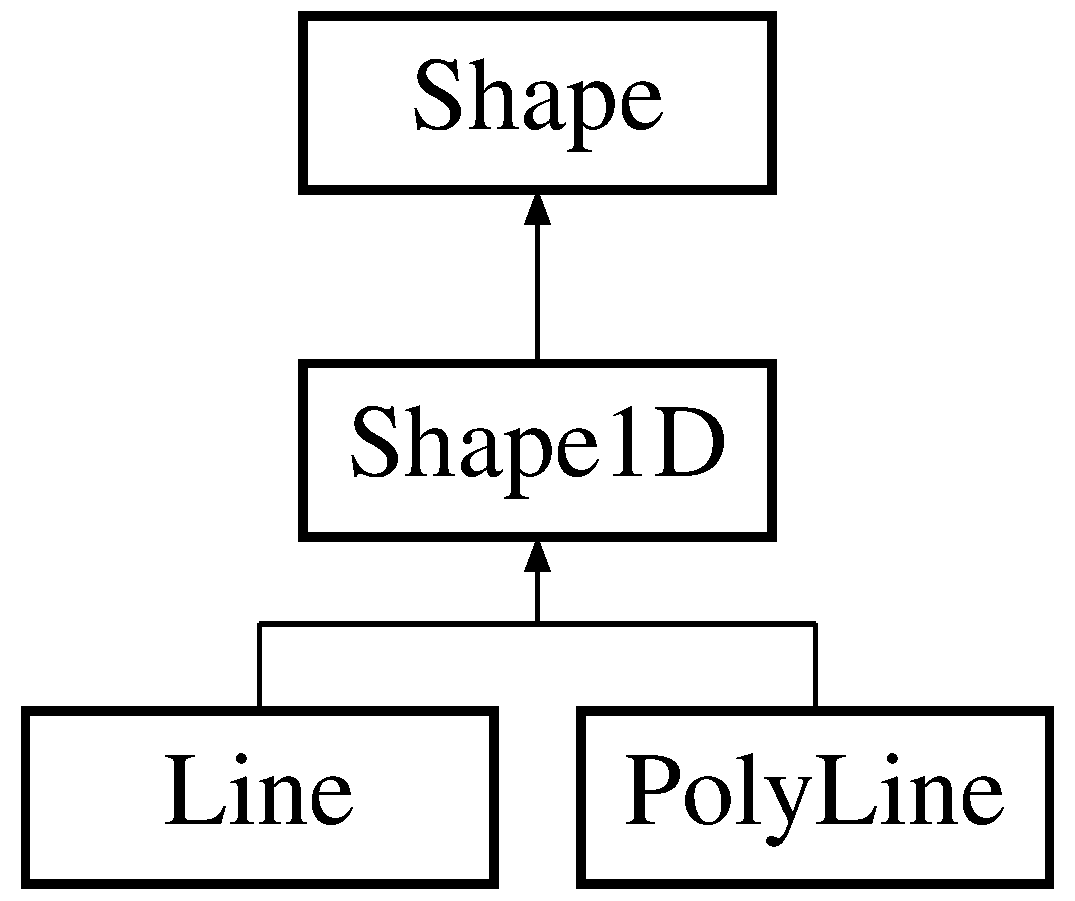
\includegraphics[height=3.000000cm]{classShape1D}
\end{center}
\end{figure}
\subsection*{Public Member Functions}
\begin{DoxyCompactItemize}
\item 
\hyperlink{classShape1D_a2dd4df43f1a9c8530e5346465f638011}{Shape1\-D} (Q\-Paint\-Device $\ast$device, int x\-Id, \hyperlink{classShape_aaac58aa2f6760d0f06ec1710d5123e9b}{shape\-Type} x\-Type, Q\-Color x\-Pen\-Color, qreal x\-Pen\-Width, Qt\-::\-Pen\-Style x\-Pen\-Style, Qt\-::\-Pen\-Cap\-Style x\-Pen\-Cap\-Style, Qt\-::\-Pen\-Join\-Style x\-Pen\-Join\-Style)
\item 
\hypertarget{classShape1D_a58711e617f2cbc92b5732586f0ff96b8}{\hyperlink{classShape1D}{Shape1\-D} \& {\bfseries operator=} (const \hyperlink{classShape1D}{Shape1\-D} \&)=delete}\label{classShape1D_a58711e617f2cbc92b5732586f0ff96b8}

\item 
\hypertarget{classShape1D_ad0be726f3444d3d76484ce9afa3c8214}{{\bfseries Shape1\-D} (const \hyperlink{classShape1D}{Shape1\-D} \&)=delete}\label{classShape1D_ad0be726f3444d3d76484ce9afa3c8214}

\item 
virtual \hyperlink{classShape1D_aef223c181450f2dd0f304072e2fa0382}{$\sim$\-Shape1\-D} ()
\item 
virtual std\-::ostream \& \hyperlink{classShape1D_a20b9358df369b7b0fc4a1cdae5070836}{print} (std\-::ostream \&os) const =0
\end{DoxyCompactItemize}
\subsection*{Public Attributes}
\begin{DoxyCompactItemize}
\item 
\hypertarget{classShape1D_add0a527e431b0d5a216b600a2c60903a}{Q\-Pen \hyperlink{classShape1D_add0a527e431b0d5a216b600a2c60903a}{pen}}\label{classShape1D_add0a527e431b0d5a216b600a2c60903a}

\begin{DoxyCompactList}\small\item\em Pen used to draw shape outline. \end{DoxyCompactList}\item 
\hypertarget{classShape1D_a2a00297b7ebd6dcd64beb0474e6cd42d}{Q\-Point \hyperlink{classShape1D_a2a00297b7ebd6dcd64beb0474e6cd42d}{upperleft}}\label{classShape1D_a2a00297b7ebd6dcd64beb0474e6cd42d}

\begin{DoxyCompactList}\small\item\em Upper left anchor of bounding rectangle. \end{DoxyCompactList}\item 
\hypertarget{classShape1D_a5783a298129c1797b89c38fba3ab1888}{Q\-Point \hyperlink{classShape1D_a5783a298129c1797b89c38fba3ab1888}{lowerright}}\label{classShape1D_a5783a298129c1797b89c38fba3ab1888}

\begin{DoxyCompactList}\small\item\em Lower right anchor for bounding rectangle. \end{DoxyCompactList}\item 
\hypertarget{classShape1D_a5cafd442acdfe031e4fd9db08a119e23}{std\-::vector$<$ Q\-Point $>$ \hyperlink{classShape1D_a5cafd442acdfe031e4fd9db08a119e23}{points}}\label{classShape1D_a5cafd442acdfe031e4fd9db08a119e23}

\begin{DoxyCompactList}\small\item\em vector containing endpints and vertices of line objects \end{DoxyCompactList}\end{DoxyCompactItemize}
\subsection*{Additional Inherited Members}


\subsection{Constructor \& Destructor Documentation}
\hypertarget{classShape1D_a2dd4df43f1a9c8530e5346465f638011}{\index{Shape1\-D@{Shape1\-D}!Shape1\-D@{Shape1\-D}}
\index{Shape1\-D@{Shape1\-D}!Shape1D@{Shape1\-D}}
\subsubsection[{Shape1\-D}]{\setlength{\rightskip}{0pt plus 5cm}Shape1\-D\-::\-Shape1\-D (
\begin{DoxyParamCaption}
\item[{Q\-Paint\-Device $\ast$}]{device, }
\item[{int}]{x\-Id, }
\item[{{\bf shape\-Type}}]{x\-Type, }
\item[{Q\-Color}]{x\-Pen\-Color, }
\item[{qreal}]{x\-Pen\-Width, }
\item[{Qt\-::\-Pen\-Style}]{x\-Pen\-Style, }
\item[{Qt\-::\-Pen\-Cap\-Style}]{x\-Pen\-Cap\-Style, }
\item[{Qt\-::\-Pen\-Join\-Style}]{x\-Pen\-Join\-Style}
\end{DoxyParamCaption}
)\hspace{0.3cm}{\ttfamily [inline]}}}\label{classShape1D_a2dd4df43f1a9c8530e5346465f638011}
Constructor -\/ abstract class for 1\-D (line) objects

\begin{DoxyAuthor}{Author}
edt (5/14/18)
\end{DoxyAuthor}

\begin{DoxyParams}{Parameters}
{\em device} & -\/ Q\-Paint\-Device \\
\hline
{\em x\-Id} & -\/ shape I\-D \\
\hline
{\em x\-Type} & \\
\hline
{\em x\-Pen\-Color} & \\
\hline
{\em x\-Pen\-Width} & \\
\hline
{\em x\-Pen\-Style} & \\
\hline
{\em x\-Pen\-Cap\-Style} & \\
\hline
{\em x\-Pen\-Join\-Style} & \\
\hline
\end{DoxyParams}
\hypertarget{classShape1D_aef223c181450f2dd0f304072e2fa0382}{\index{Shape1\-D@{Shape1\-D}!$\sim$\-Shape1\-D@{$\sim$\-Shape1\-D}}
\index{$\sim$\-Shape1\-D@{$\sim$\-Shape1\-D}!Shape1D@{Shape1\-D}}
\subsubsection[{$\sim$\-Shape1\-D}]{\setlength{\rightskip}{0pt plus 5cm}virtual Shape1\-D\-::$\sim$\-Shape1\-D (
\begin{DoxyParamCaption}
{}
\end{DoxyParamCaption}
)\hspace{0.3cm}{\ttfamily [inline]}, {\ttfamily [virtual]}}}\label{classShape1D_aef223c181450f2dd0f304072e2fa0382}
Destructor -\/ simply free the object space

\begin{DoxyAuthor}{Author}
edt (5/13/18) 
\end{DoxyAuthor}


\subsection{Member Function Documentation}
\hypertarget{classShape1D_a20b9358df369b7b0fc4a1cdae5070836}{\index{Shape1\-D@{Shape1\-D}!print@{print}}
\index{print@{print}!Shape1D@{Shape1\-D}}
\subsubsection[{print}]{\setlength{\rightskip}{0pt plus 5cm}virtual std\-::ostream\& Shape1\-D\-::print (
\begin{DoxyParamCaption}
\item[{std\-::ostream \&}]{os}
\end{DoxyParamCaption}
) const\hspace{0.3cm}{\ttfamily [pure virtual]}}}\label{classShape1D_a20b9358df369b7b0fc4a1cdae5070836}
print -\/ print limited information about derived instance for debugging

\begin{DoxyAuthor}{Author}
edt (5/13/18)
\end{DoxyAuthor}

\begin{DoxyParams}{Parameters}
{\em os} & -\/ output stream\\
\hline
\end{DoxyParams}
\begin{DoxyReturn}{Returns}
std\-::ostream\& 
\end{DoxyReturn}


Implements \hyperlink{classShape}{Shape}.



Implemented in \hyperlink{classLine_a9535dc5fe2c3e66e548add6622e4b0ea}{Line}, and \hyperlink{classPolyLine_a716cc39a1e35f7538013760b0828aee6}{Poly\-Line}.



The documentation for this class was generated from the following file\-:\begin{DoxyCompactItemize}
\item 
/home/edt/\-C\-S1\-C/\-Class\-Project/\-Main\-Window/shape1d.\-h\end{DoxyCompactItemize}

\hypertarget{classShape2D}{\section{Shape2\-D Class Reference}
\label{classShape2D}\index{Shape2\-D@{Shape2\-D}}
}
Inheritance diagram for Shape2\-D\-:\begin{figure}[H]
\begin{center}
\leavevmode
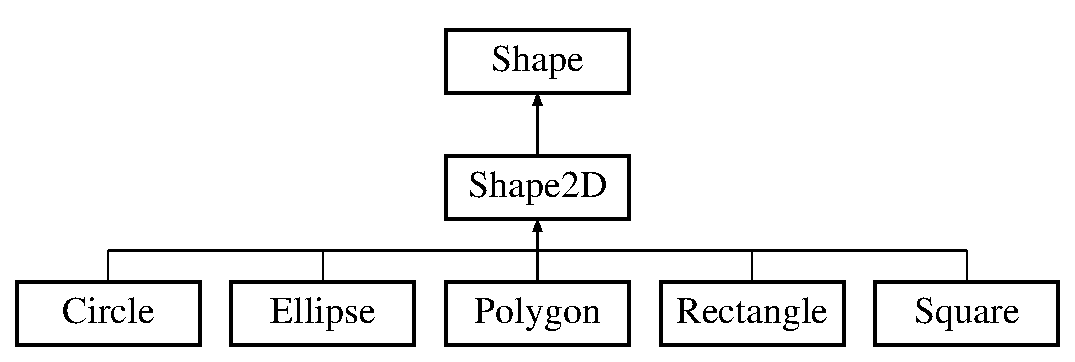
\includegraphics[height=3.000000cm]{classShape2D}
\end{center}
\end{figure}
\subsection*{Public Member Functions}
\begin{DoxyCompactItemize}
\item 
\hyperlink{classShape2D_ac890aa93495c70461761925145232d11}{Shape2\-D} (Q\-Paint\-Device $\ast$device, int x\-Id, \hyperlink{classShape_aaac58aa2f6760d0f06ec1710d5123e9b}{shape\-Type} x\-Type, Q\-Color x\-Pen\-Color, qreal x\-Pen\-Width, Qt\-::\-Pen\-Style x\-Pen\-Style, Qt\-::\-Pen\-Cap\-Style x\-Pen\-Cap\-Style, Qt\-::\-Pen\-Join\-Style x\-Pen\-Join\-Style, Q\-Color x\-Brush\-Color, Qt\-::\-Brush\-Style x\-Brush\-Style)
\item 
\hypertarget{classShape2D_a54dbc4873b59a4521937add746c2153e}{\hyperlink{classShape2D}{Shape2\-D} \& {\bfseries operator=} (const \hyperlink{classShape}{Shape} \&)=delete}\label{classShape2D_a54dbc4873b59a4521937add746c2153e}

\item 
\hypertarget{classShape2D_ae8b380001f180357fa4e80196eb3d20b}{{\bfseries Shape2\-D} (const \hyperlink{classShape}{Shape} \&)=delete}\label{classShape2D_ae8b380001f180357fa4e80196eb3d20b}

\item 
virtual \hyperlink{classShape2D_ad151443d27b1861c3de7b6b7147c1019}{$\sim$\-Shape2\-D} ()
\item 
virtual std\-::ostream \& \hyperlink{classShape2D_a6faf0b7950ea77a2ec6f29a31d65a624}{print} (std\-::ostream \&os) const =0
\end{DoxyCompactItemize}
\subsection*{Public Attributes}
\begin{DoxyCompactItemize}
\item 
\hypertarget{classShape2D_a703b6a05045fdfdd01a362fe80c6db73}{Q\-Pen \hyperlink{classShape2D_a703b6a05045fdfdd01a362fe80c6db73}{pen}}\label{classShape2D_a703b6a05045fdfdd01a362fe80c6db73}

\begin{DoxyCompactList}\small\item\em Pen used to draw shape outline. \end{DoxyCompactList}\item 
\hypertarget{classShape2D_ad2a39e54a4cce0f95547225ad6282f54}{Q\-Brush \hyperlink{classShape2D_ad2a39e54a4cce0f95547225ad6282f54}{brush}}\label{classShape2D_ad2a39e54a4cce0f95547225ad6282f54}

\begin{DoxyCompactList}\small\item\em Brush used to fill 2\-D object interior. \end{DoxyCompactList}\item 
\hypertarget{classShape2D_a04ff6cd950715ef89ecea1d4004e2cab}{Q\-Point \hyperlink{classShape2D_a04ff6cd950715ef89ecea1d4004e2cab}{upperleft}}\label{classShape2D_a04ff6cd950715ef89ecea1d4004e2cab}

\begin{DoxyCompactList}\small\item\em Lower right anchor for bounding rectangle. \end{DoxyCompactList}\item 
\hypertarget{classShape2D_ac09b295b11d1668f6c696ac8480e9466}{Q\-Point \hyperlink{classShape2D_ac09b295b11d1668f6c696ac8480e9466}{lowerright}}\label{classShape2D_ac09b295b11d1668f6c696ac8480e9466}

\begin{DoxyCompactList}\small\item\em vector containing endpints and vertices of line objects \end{DoxyCompactList}\end{DoxyCompactItemize}
\subsection*{Additional Inherited Members}


\subsection{Constructor \& Destructor Documentation}
\hypertarget{classShape2D_ac890aa93495c70461761925145232d11}{\index{Shape2\-D@{Shape2\-D}!Shape2\-D@{Shape2\-D}}
\index{Shape2\-D@{Shape2\-D}!Shape2D@{Shape2\-D}}
\subsubsection[{Shape2\-D}]{\setlength{\rightskip}{0pt plus 5cm}Shape2\-D\-::\-Shape2\-D (
\begin{DoxyParamCaption}
\item[{Q\-Paint\-Device $\ast$}]{device, }
\item[{int}]{x\-Id, }
\item[{{\bf shape\-Type}}]{x\-Type, }
\item[{Q\-Color}]{x\-Pen\-Color, }
\item[{qreal}]{x\-Pen\-Width, }
\item[{Qt\-::\-Pen\-Style}]{x\-Pen\-Style, }
\item[{Qt\-::\-Pen\-Cap\-Style}]{x\-Pen\-Cap\-Style, }
\item[{Qt\-::\-Pen\-Join\-Style}]{x\-Pen\-Join\-Style, }
\item[{Q\-Color}]{x\-Brush\-Color, }
\item[{Qt\-::\-Brush\-Style}]{x\-Brush\-Style}
\end{DoxyParamCaption}
)\hspace{0.3cm}{\ttfamily [inline]}}}\label{classShape2D_ac890aa93495c70461761925145232d11}
Constructor -\/ abstract class for 2\-D (circle, square, etc) objects

\begin{DoxyAuthor}{Author}
edt (5/14/18)
\end{DoxyAuthor}

\begin{DoxyParams}{Parameters}
{\em device} & -\/ Q\-Paint\-Device \\
\hline
{\em x\-Id} & -\/ shape I\-D \\
\hline
{\em x\-Type} & \\
\hline
{\em x\-Pen\-Color} & \\
\hline
{\em x\-Pen\-Width} & \\
\hline
{\em x\-Pen\-Style} & \\
\hline
{\em x\-Pen\-Cap\-Style} & \\
\hline
{\em x\-Pen\-Join\-Style} & \\
\hline
{\em x\-Brush\-Color} & \\
\hline
{\em x\-Brush\-Style} & \\
\hline
\end{DoxyParams}
\hypertarget{classShape2D_ad151443d27b1861c3de7b6b7147c1019}{\index{Shape2\-D@{Shape2\-D}!$\sim$\-Shape2\-D@{$\sim$\-Shape2\-D}}
\index{$\sim$\-Shape2\-D@{$\sim$\-Shape2\-D}!Shape2D@{Shape2\-D}}
\subsubsection[{$\sim$\-Shape2\-D}]{\setlength{\rightskip}{0pt plus 5cm}virtual Shape2\-D\-::$\sim$\-Shape2\-D (
\begin{DoxyParamCaption}
{}
\end{DoxyParamCaption}
)\hspace{0.3cm}{\ttfamily [inline]}, {\ttfamily [virtual]}}}\label{classShape2D_ad151443d27b1861c3de7b6b7147c1019}
Destructor -\/ simply free the object space

\begin{DoxyAuthor}{Author}
edt (5/13/18) 
\end{DoxyAuthor}


\subsection{Member Function Documentation}
\hypertarget{classShape2D_a6faf0b7950ea77a2ec6f29a31d65a624}{\index{Shape2\-D@{Shape2\-D}!print@{print}}
\index{print@{print}!Shape2D@{Shape2\-D}}
\subsubsection[{print}]{\setlength{\rightskip}{0pt plus 5cm}virtual std\-::ostream\& Shape2\-D\-::print (
\begin{DoxyParamCaption}
\item[{std\-::ostream \&}]{os}
\end{DoxyParamCaption}
) const\hspace{0.3cm}{\ttfamily [pure virtual]}}}\label{classShape2D_a6faf0b7950ea77a2ec6f29a31d65a624}
print -\/ print limited information about derived instance for debugging

\begin{DoxyAuthor}{Author}
edt (5/13/18)
\end{DoxyAuthor}

\begin{DoxyParams}{Parameters}
{\em os} & -\/ output stream\\
\hline
\end{DoxyParams}
\begin{DoxyReturn}{Returns}
std\-::ostream\& 
\end{DoxyReturn}


Implements \hyperlink{classShape}{Shape}.



Implemented in \hyperlink{classRectangle_a06528cd92243f56f5eca551c5d637657}{Rectangle}, \hyperlink{classEllipse_a6cd8da652c6e66f465fb23253deab458}{Ellipse}, \hyperlink{classCircle_a8afb61e2e5b24c95d0d4514da1d45bb2}{Circle}, \hyperlink{classPolygon_ae1d7135748131313fac844463013931e}{Polygon}, and \hyperlink{classSquare_af2b00ed5022d4eefcbafe31cc77535f6}{Square}.



The documentation for this class was generated from the following file\-:\begin{DoxyCompactItemize}
\item 
/home/edt/\-C\-S1\-C/\-Class\-Project/\-Main\-Window/shape2d.\-h\end{DoxyCompactItemize}

\hypertarget{classSquare}{\section{Square Class Reference}
\label{classSquare}\index{Square@{Square}}
}
Inheritance diagram for Square\-:\begin{figure}[H]
\begin{center}
\leavevmode
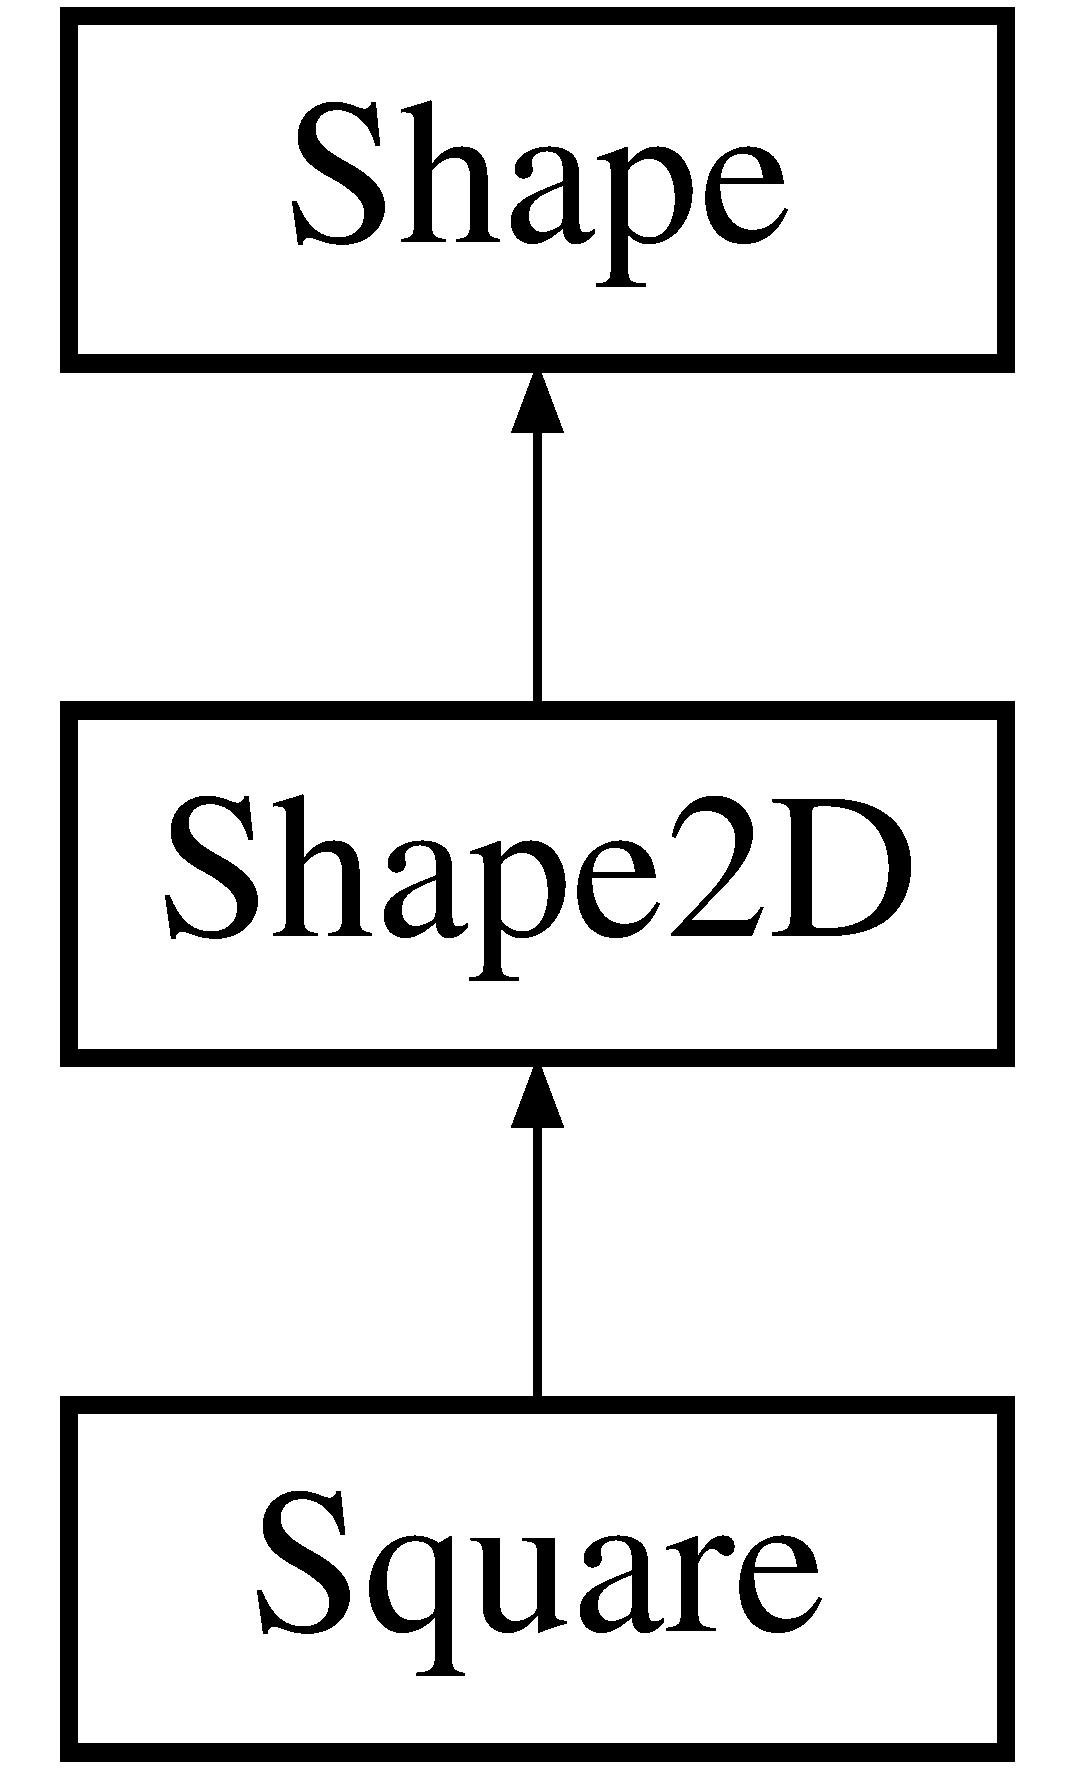
\includegraphics[height=3.000000cm]{classSquare}
\end{center}
\end{figure}
\subsection*{Public Member Functions}
\begin{DoxyCompactItemize}
\item 
\hyperlink{classSquare_aa8ee6128744d0bf3bc697c035acf4441}{Square} (Q\-Paint\-Device $\ast$device, int x\-Id, Q\-Color x\-Pen\-Color, qreal x\-Pen\-Width, Qt\-::\-Pen\-Style x\-Pen\-Style, Qt\-::\-Pen\-Cap\-Style x\-Pen\-Cap\-Style, Qt\-::\-Pen\-Join\-Style x\-Pen\-Join\-Style, Q\-Color x\-Brush\-Color, Qt\-::\-Brush\-Style x\-Brush\-Style, int x\-Top\-Left\-X, int x\-Top\-Left\-Y, int x\-Side)
\item 
\hypertarget{classSquare_abea50130b033d31a45d1ec4fa2c3aab6}{\hyperlink{classSquare}{Square} \& {\bfseries operator=} (const \hyperlink{classSquare}{Square} \&)=delete}\label{classSquare_abea50130b033d31a45d1ec4fa2c3aab6}

\item 
\hypertarget{classSquare_a0b76cd4153675ea610cd495a2eabbd65}{{\bfseries Square} (const \hyperlink{classSquare}{Square} \&)=delete}\label{classSquare_a0b76cd4153675ea610cd495a2eabbd65}

\item 
\hyperlink{classSquare_a90af7ce1060cff7b717ceddb333846b8}{$\sim$\-Square} ()
\item 
std\-::ostream \& \hyperlink{classSquare_af2b00ed5022d4eefcbafe31cc77535f6}{print} (std\-::ostream \&os) const 
\item 
void \hyperlink{classSquare_aa7119d995068a665c84712f1673cf413}{draw} (Q\-Paint\-Device $\ast$device)
\item 
void \hyperlink{classSquare_a90610398a48ef62bb9d948c37d2ec7cc}{move} (Q\-Point \&new\-Upper\-Left)
\item 
void \hyperlink{classSquare_acfd8a9b71e6cf950c34eb022cbe3ae11}{update} (void)
\item 
double \hyperlink{classSquare_adc4486c61e47855be176c4c38db7e2df}{calc\-Perimeter} () const 
\item 
double \hyperlink{classSquare_a203f54d90c5c3282579725ca8354d882}{calc\-Area} () const 
\end{DoxyCompactItemize}
\subsection*{Additional Inherited Members}


\subsection{Constructor \& Destructor Documentation}
\hypertarget{classSquare_aa8ee6128744d0bf3bc697c035acf4441}{\index{Square@{Square}!Square@{Square}}
\index{Square@{Square}!Square@{Square}}
\subsubsection[{Square}]{\setlength{\rightskip}{0pt plus 5cm}Square\-::\-Square (
\begin{DoxyParamCaption}
\item[{Q\-Paint\-Device $\ast$}]{device, }
\item[{int}]{x\-Id, }
\item[{Q\-Color}]{x\-Pen\-Color, }
\item[{qreal}]{x\-Pen\-Width, }
\item[{Qt\-::\-Pen\-Style}]{x\-Pen\-Style, }
\item[{Qt\-::\-Pen\-Cap\-Style}]{x\-Pen\-Cap\-Style, }
\item[{Qt\-::\-Pen\-Join\-Style}]{x\-Pen\-Join\-Style, }
\item[{Q\-Color}]{x\-Brush\-Color, }
\item[{Qt\-::\-Brush\-Style}]{x\-Brush\-Style, }
\item[{int}]{x\-Top\-Left\-X, }
\item[{int}]{x\-Top\-Left\-Y, }
\item[{int}]{x\-Side}
\end{DoxyParamCaption}
)}}\label{classSquare_aa8ee6128744d0bf3bc697c035acf4441}
Constructor -\/ create a Q\-T drawable square 2\-D

\begin{DoxyAuthor}{Author}
edt (5/14/18)
\end{DoxyAuthor}

\begin{DoxyParams}{Parameters}
{\em device} & -\/ Q\-Paint\-Device \\
\hline
{\em x\-Id} & -\/ shape I\-D \\
\hline
{\em x\-Pen\-Color} & \\
\hline
{\em x\-Pen\-Width} & \\
\hline
{\em x\-Pen\-Style} & \\
\hline
{\em x\-Pen\-Cap\-Style} & \\
\hline
{\em x\-Pen\-Join\-Style} & \\
\hline
{\em x\-Brush\-Color} & \\
\hline
{\em x\-Brush\-Style} & \\
\hline
{\em x\-Top\-Left\-X} & \\
\hline
{\em x\-Top\-Left\-Y} & \\
\hline
{\em x\-Side} & \\
\hline
\end{DoxyParams}
\hypertarget{classSquare_a90af7ce1060cff7b717ceddb333846b8}{\index{Square@{Square}!$\sim$\-Square@{$\sim$\-Square}}
\index{$\sim$\-Square@{$\sim$\-Square}!Square@{Square}}
\subsubsection[{$\sim$\-Square}]{\setlength{\rightskip}{0pt plus 5cm}Square\-::$\sim$\-Square (
\begin{DoxyParamCaption}
{}
\end{DoxyParamCaption}
)}}\label{classSquare_a90af7ce1060cff7b717ceddb333846b8}
Destructor -\/ simply free the object space

\begin{DoxyAuthor}{Author}
edt (5/13/18) 
\end{DoxyAuthor}


\subsection{Member Function Documentation}
\hypertarget{classSquare_a203f54d90c5c3282579725ca8354d882}{\index{Square@{Square}!calc\-Area@{calc\-Area}}
\index{calc\-Area@{calc\-Area}!Square@{Square}}
\subsubsection[{calc\-Area}]{\setlength{\rightskip}{0pt plus 5cm}double Square\-::calc\-Area (
\begin{DoxyParamCaption}
\item[{void}]{}
\end{DoxyParamCaption}
) const\hspace{0.3cm}{\ttfamily [virtual]}}}\label{classSquare_a203f54d90c5c3282579725ca8354d882}
calc\-Area -\/ determine area enclosed by object

\begin{DoxyAuthor}{Author}
edt (5/13/18)
\end{DoxyAuthor}
\begin{DoxyReturn}{Returns}
double 
\end{DoxyReturn}


Implements \hyperlink{classShape}{Shape}.

\hypertarget{classSquare_adc4486c61e47855be176c4c38db7e2df}{\index{Square@{Square}!calc\-Perimeter@{calc\-Perimeter}}
\index{calc\-Perimeter@{calc\-Perimeter}!Square@{Square}}
\subsubsection[{calc\-Perimeter}]{\setlength{\rightskip}{0pt plus 5cm}double Square\-::calc\-Perimeter (
\begin{DoxyParamCaption}
\item[{void}]{}
\end{DoxyParamCaption}
) const\hspace{0.3cm}{\ttfamily [virtual]}}}\label{classSquare_adc4486c61e47855be176c4c38db7e2df}
calc\-Perimeter -\/ determine object outline length

\begin{DoxyAuthor}{Author}
edt (5/13/18)
\end{DoxyAuthor}
\begin{DoxyReturn}{Returns}
double 
\end{DoxyReturn}


Implements \hyperlink{classShape}{Shape}.

\hypertarget{classSquare_aa7119d995068a665c84712f1673cf413}{\index{Square@{Square}!draw@{draw}}
\index{draw@{draw}!Square@{Square}}
\subsubsection[{draw}]{\setlength{\rightskip}{0pt plus 5cm}void Square\-::draw (
\begin{DoxyParamCaption}
\item[{Q\-Paint\-Device $\ast$}]{device}
\end{DoxyParamCaption}
)\hspace{0.3cm}{\ttfamily [virtual]}}}\label{classSquare_aa7119d995068a665c84712f1673cf413}
draw -\/ output object onto Q\-T canvas using Q\-Paint\-Device

\begin{DoxyAuthor}{Author}
edt (5/13/18)
\end{DoxyAuthor}

\begin{DoxyParams}{Parameters}
{\em device} & \\
\hline
\end{DoxyParams}


Implements \hyperlink{classShape}{Shape}.

\hypertarget{classSquare_a90610398a48ef62bb9d948c37d2ec7cc}{\index{Square@{Square}!move@{move}}
\index{move@{move}!Square@{Square}}
\subsubsection[{move}]{\setlength{\rightskip}{0pt plus 5cm}void Square\-::move (
\begin{DoxyParamCaption}
\item[{Q\-Point \&}]{new\-Upper\-Left}
\end{DoxyParamCaption}
)\hspace{0.3cm}{\ttfamily [virtual]}}}\label{classSquare_a90610398a48ef62bb9d948c37d2ec7cc}
move -\/ relocate square to new upper left coordinate

\begin{DoxyAuthor}{Author}
edt (5/13/18)
\end{DoxyAuthor}

\begin{DoxyParams}{Parameters}
{\em new\-Upper\-Left} & -\/ new location of upper left of enclosing rectangle \\
\hline
\end{DoxyParams}


Implements \hyperlink{classShape}{Shape}.

\hypertarget{classSquare_af2b00ed5022d4eefcbafe31cc77535f6}{\index{Square@{Square}!print@{print}}
\index{print@{print}!Square@{Square}}
\subsubsection[{print}]{\setlength{\rightskip}{0pt plus 5cm}std\-::ostream \& Square\-::print (
\begin{DoxyParamCaption}
\item[{std\-::ostream \&}]{os}
\end{DoxyParamCaption}
) const\hspace{0.3cm}{\ttfamily [virtual]}}}\label{classSquare_af2b00ed5022d4eefcbafe31cc77535f6}
print -\/ print limited information about derived instance for debugging

\begin{DoxyAuthor}{Author}
edt (5/13/18)
\end{DoxyAuthor}

\begin{DoxyParams}{Parameters}
{\em os} & -\/ output stream\\
\hline
\end{DoxyParams}
\begin{DoxyReturn}{Returns}
std\-::ostream\& 
\end{DoxyReturn}


Implements \hyperlink{classShape2D_a6faf0b7950ea77a2ec6f29a31d65a624}{Shape2\-D}.

\hypertarget{classSquare_acfd8a9b71e6cf950c34eb022cbe3ae11}{\index{Square@{Square}!update@{update}}
\index{update@{update}!Square@{Square}}
\subsubsection[{update}]{\setlength{\rightskip}{0pt plus 5cm}void Square\-::update (
\begin{DoxyParamCaption}
\item[{void}]{}
\end{DoxyParamCaption}
)\hspace{0.3cm}{\ttfamily [virtual]}}}\label{classSquare_acfd8a9b71e6cf950c34eb022cbe3ae11}
update -\/ force redraw of object

\begin{DoxyAuthor}{Author}
edt (5/13/18) 
\end{DoxyAuthor}


Implements \hyperlink{classShape}{Shape}.



The documentation for this class was generated from the following files\-:\begin{DoxyCompactItemize}
\item 
/home/edt/\-C\-S1\-C/\-Class\-Project/\-Main\-Window/square.\-h\item 
/home/edt/\-C\-S1\-C/\-Class\-Project/\-Main\-Window/square.\-cpp\end{DoxyCompactItemize}

\hypertarget{classtestimonials}{\section{testimonials Class Reference}
\label{classtestimonials}\index{testimonials@{testimonials}}
}


{\ttfamily \#include $<$testimonials.\-h$>$}

Inheritance diagram for testimonials\-:\begin{figure}[H]
\begin{center}
\leavevmode
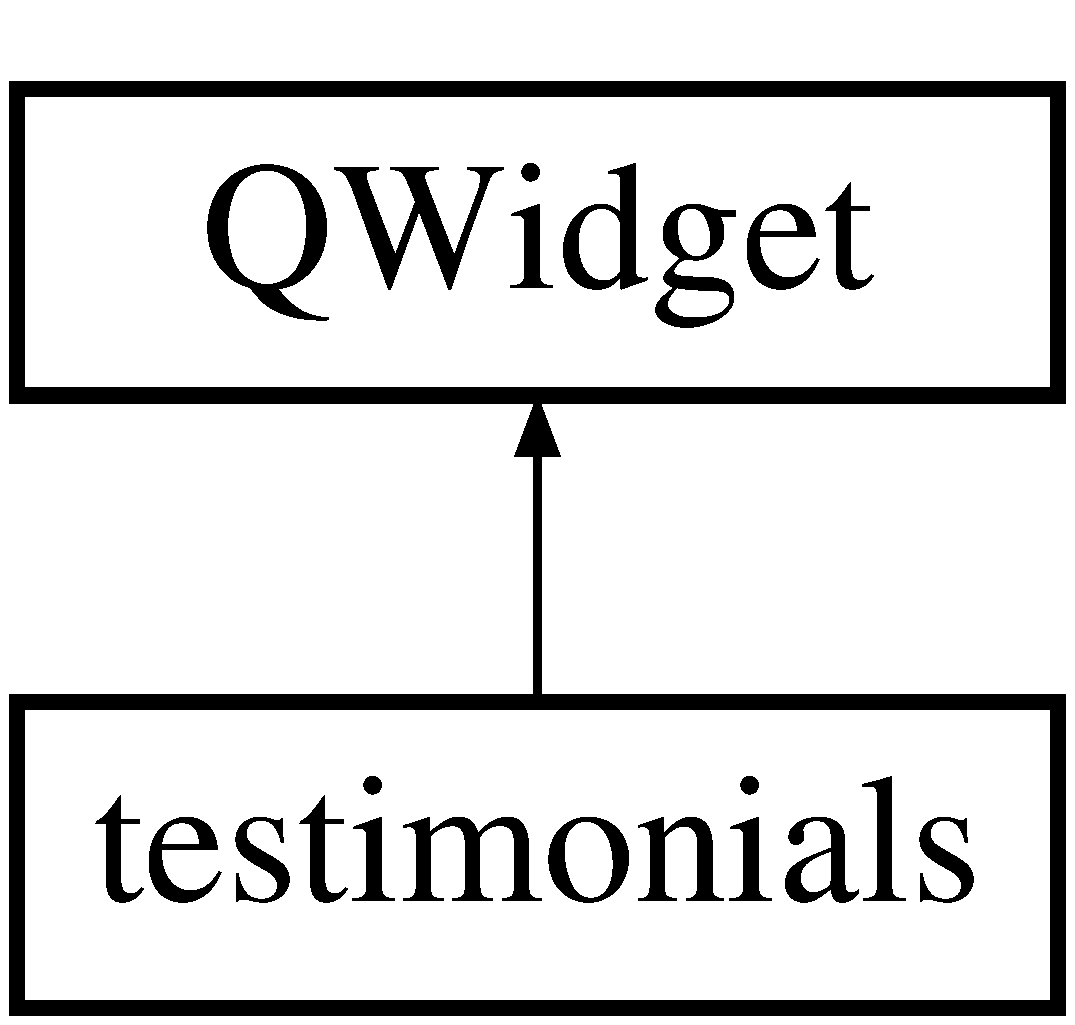
\includegraphics[height=2.000000cm]{classtestimonials}
\end{center}
\end{figure}
\subsection*{Public Member Functions}
\begin{DoxyCompactItemize}
\item 
\hyperlink{classtestimonials_aeda8ceffc4fc863bade365d69f75e9f2}{testimonials} (Q\-Widget $\ast$parent=0)
\item 
void \hyperlink{classtestimonials_af31e58ff3498d9fac55aeb1f4aaaff8a}{show\-Event} (Q\-Show\-Event $\ast$event)
\item 
\hyperlink{classtestimonials_a5946a6a44f2fffa492fa340245f49190}{$\sim$testimonials} ()
\item 
void \hyperlink{classtestimonials_af04e654a01033ca548d34aff2d84a948}{update\-Testimonies} ()
\end{DoxyCompactItemize}


\subsection{Detailed Description}
Testimonials Class -\/ holds information for the testimonials dialog

\begin{DoxyAuthor}{Author}
richard (5/14/18) 
\end{DoxyAuthor}


\subsection{Constructor \& Destructor Documentation}
\hypertarget{classtestimonials_aeda8ceffc4fc863bade365d69f75e9f2}{\index{testimonials@{testimonials}!testimonials@{testimonials}}
\index{testimonials@{testimonials}!testimonials@{testimonials}}
\subsubsection[{testimonials}]{\setlength{\rightskip}{0pt plus 5cm}testimonials\-::testimonials (
\begin{DoxyParamCaption}
\item[{Q\-Widget $\ast$}]{parent = {\ttfamily 0}}
\end{DoxyParamCaption}
)\hspace{0.3cm}{\ttfamily [explicit]}}}\label{classtestimonials_aeda8ceffc4fc863bade365d69f75e9f2}
testimonials constructor -\/ requires a Q\-Widget to draw on

\begin{DoxyAuthor}{Author}
richard (5/14/18)
\end{DoxyAuthor}

\begin{DoxyParams}{Parameters}
{\em parent} & \\
\hline
\end{DoxyParams}
\hypertarget{classtestimonials_a5946a6a44f2fffa492fa340245f49190}{\index{testimonials@{testimonials}!$\sim$testimonials@{$\sim$testimonials}}
\index{$\sim$testimonials@{$\sim$testimonials}!testimonials@{testimonials}}
\subsubsection[{$\sim$testimonials}]{\setlength{\rightskip}{0pt plus 5cm}testimonials\-::$\sim$testimonials (
\begin{DoxyParamCaption}
{}
\end{DoxyParamCaption}
)}}\label{classtestimonials_a5946a6a44f2fffa492fa340245f49190}
testimonials destructor -\/ release allocated space

\begin{DoxyAuthor}{Author}
richard (5/14/18) 
\end{DoxyAuthor}


\subsection{Member Function Documentation}
\hypertarget{classtestimonials_af31e58ff3498d9fac55aeb1f4aaaff8a}{\index{testimonials@{testimonials}!show\-Event@{show\-Event}}
\index{show\-Event@{show\-Event}!testimonials@{testimonials}}
\subsubsection[{show\-Event}]{\setlength{\rightskip}{0pt plus 5cm}void testimonials\-::show\-Event (
\begin{DoxyParamCaption}
\item[{Q\-Show\-Event $\ast$}]{event}
\end{DoxyParamCaption}
)}}\label{classtestimonials_af31e58ff3498d9fac55aeb1f4aaaff8a}
show\-Event -\/ make changes to window visible immediately -\/ Overlaods Q\-Widgit //! -\/ Calls previous show\-Event, and A\-L\-S\-O update\-Testimonie

\begin{DoxyAuthor}{Author}
richard (5/14/18)
\end{DoxyAuthor}

\begin{DoxyParams}{Parameters}
{\em event} & \\
\hline
\end{DoxyParams}
\hypertarget{classtestimonials_af04e654a01033ca548d34aff2d84a948}{\index{testimonials@{testimonials}!update\-Testimonies@{update\-Testimonies}}
\index{update\-Testimonies@{update\-Testimonies}!testimonials@{testimonials}}
\subsubsection[{update\-Testimonies}]{\setlength{\rightskip}{0pt plus 5cm}void testimonials\-::update\-Testimonies (
\begin{DoxyParamCaption}
{}
\end{DoxyParamCaption}
)}}\label{classtestimonials_af04e654a01033ca548d34aff2d84a948}
update\-Testimonies -\/ Reads input from file and parses it to display as testimonial

\begin{DoxyAuthor}{Author}
richard (5/14/18) 
\end{DoxyAuthor}


The documentation for this class was generated from the following files\-:\begin{DoxyCompactItemize}
\item 
/home/edt/\-C\-S1\-C/\-Class\-Project/\-Main\-Window/testimonials.\-h\item 
/home/edt/\-C\-S1\-C/\-Class\-Project/\-Main\-Window/testimonials.\-cpp\end{DoxyCompactItemize}

\hypertarget{classText}{\section{Text Class Reference}
\label{classText}\index{Text@{Text}}
}
Inheritance diagram for Text\-:\begin{figure}[H]
\begin{center}
\leavevmode
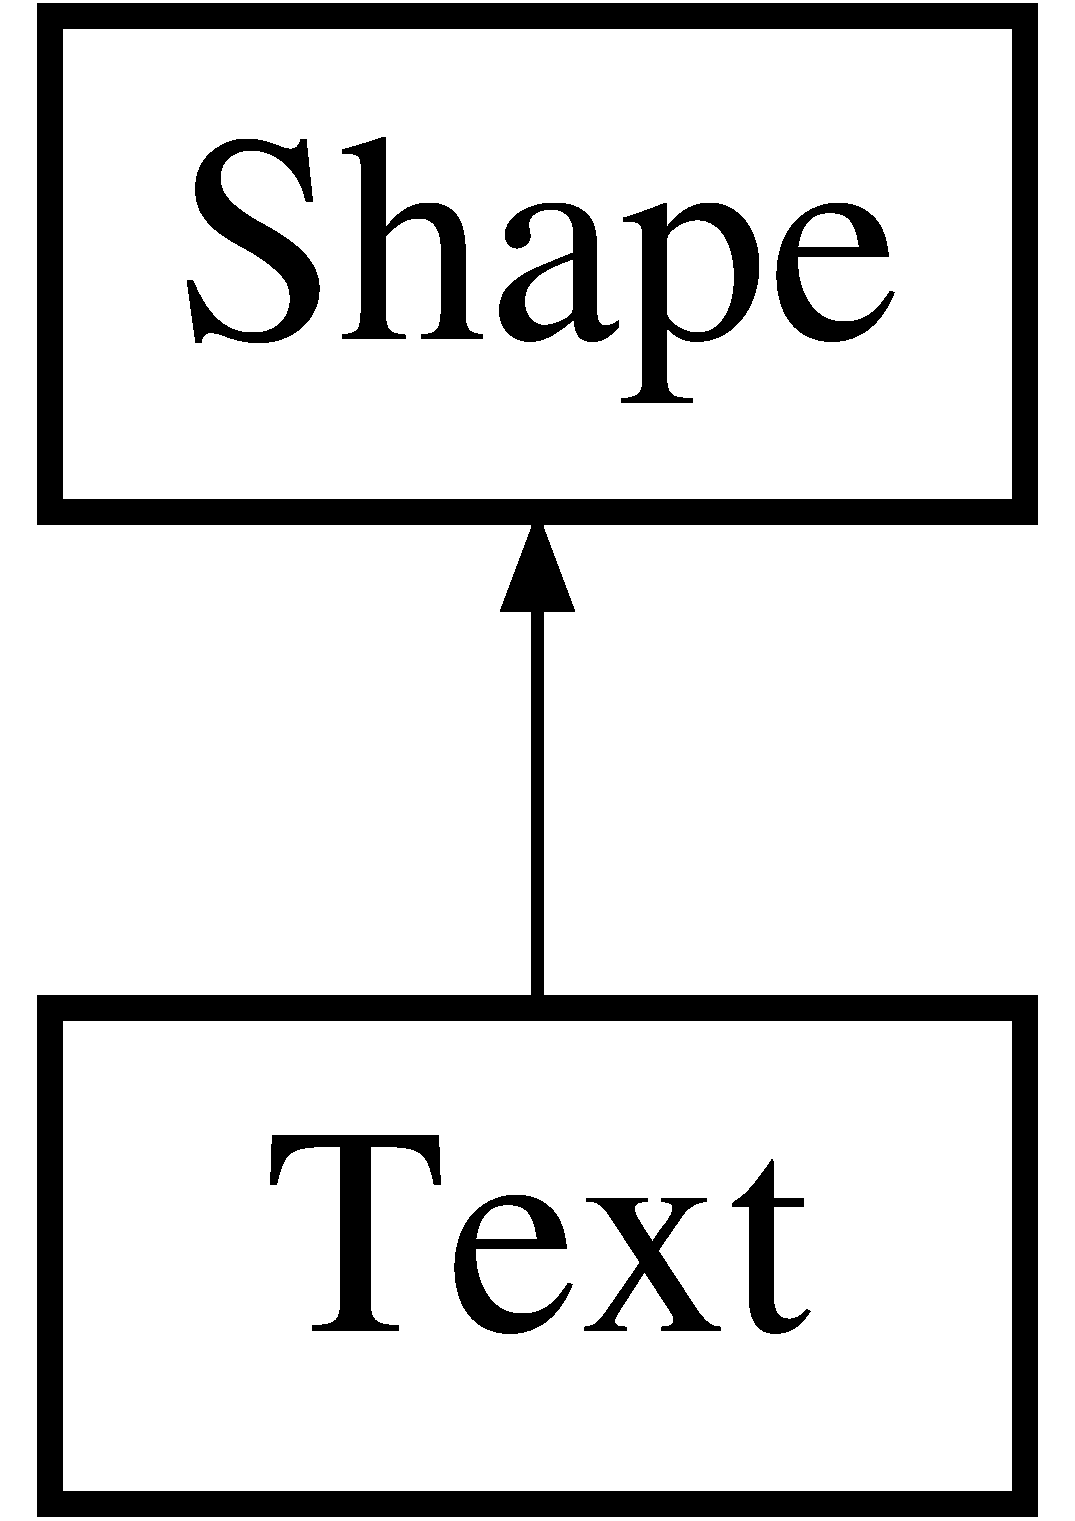
\includegraphics[height=2.000000cm]{classText}
\end{center}
\end{figure}
\subsection*{Public Member Functions}
\begin{DoxyCompactItemize}
\item 
\hyperlink{classText_a33b6e89d37f8d0db9abaa02a82a5d7ed}{Text} (Q\-Paint\-Device $\ast$device, int x\-Id, Q\-String x\-String, Q\-Color x\-Color, Qt\-::\-Alignment\-Flag x\-Alignment, int x\-Font\-Size, Q\-String x\-Font\-Family, Q\-Font\-::\-Style x\-Font\-Style, Q\-Font\-::\-Weight x\-Font\-Weight, int x\-Top\-Left\-X, int x\-Top\-Left\-Y, int x\-Width, int x\-Height)
\item 
\hypertarget{classText_ae3709f44652cc1623ba2e12fd01aa983}{\hyperlink{classText}{Text} \& {\bfseries operator=} (const \hyperlink{classText}{Text} \&)=delete}\label{classText_ae3709f44652cc1623ba2e12fd01aa983}

\item 
\hypertarget{classText_afc7da0fb8a91ece6da90c6876e9d9539}{{\bfseries Text} (const \hyperlink{classText}{Text} \&)=delete}\label{classText_afc7da0fb8a91ece6da90c6876e9d9539}

\item 
\hyperlink{classText_a2d49e5c280e205125b149f7777ae30c7}{$\sim$\-Text} ()
\item 
std\-::ostream \& \hyperlink{classText_a8ae9525e9734ed2b9e00aa53fb472f67}{print} (std\-::ostream \&os) const 
\item 
void \hyperlink{classText_ad6dfd5f6e6f1aa974c0ab433abbb5509}{draw} (Q\-Paint\-Device $\ast$device)
\item 
void \hyperlink{classText_a5586919a299988fdcdfd68e77915625d}{move} (Q\-Point \&new\-Upper\-Left)
\item 
void \hyperlink{classText_a04fa355437faa0911800bbf110bf8f0e}{update} (void)
\item 
double \hyperlink{classText_afa52da1ba9611cb0ae79f7a93b89388d}{calc\-Perimeter} () const 
\item 
double \hyperlink{classText_aa64572ee7df26460030d9bf116ad52c8}{calc\-Area} () const 
\end{DoxyCompactItemize}
\subsection*{Public Attributes}
\begin{DoxyCompactItemize}
\item 
\hypertarget{classText_aedb55d46b763e08f05098533acfbe22a}{Q\-String \hyperlink{classText_aedb55d46b763e08f05098533acfbe22a}{String}}\label{classText_aedb55d46b763e08f05098533acfbe22a}

\begin{DoxyCompactList}\small\item\em string to display \end{DoxyCompactList}\item 
\hypertarget{classText_a7080675fdb6da03a3d9fc141c3f9ee48}{Q\-Color \hyperlink{classText_a7080675fdb6da03a3d9fc141c3f9ee48}{Color}}\label{classText_a7080675fdb6da03a3d9fc141c3f9ee48}

\begin{DoxyCompactList}\small\item\em color of string text \end{DoxyCompactList}\item 
\hypertarget{classText_ac2f10e06ac4a483c431f7a0f5e589e0c}{Qt\-::\-Alignment\-Flag \hyperlink{classText_ac2f10e06ac4a483c431f7a0f5e589e0c}{Alignment}}\label{classText_ac2f10e06ac4a483c431f7a0f5e589e0c}

\begin{DoxyCompactList}\small\item\em alignment of string in bounding rectangle \end{DoxyCompactList}\item 
\hypertarget{classText_ada5a7bd7fd75b0c00b6343603690b40b}{int \hyperlink{classText_ada5a7bd7fd75b0c00b6343603690b40b}{Font\-Size}}\label{classText_ada5a7bd7fd75b0c00b6343603690b40b}

\begin{DoxyCompactList}\small\item\em font size of string \end{DoxyCompactList}\item 
\hypertarget{classText_a41605f83ceba0843f91b4cbbb62c16e2}{Q\-String \hyperlink{classText_a41605f83ceba0843f91b4cbbb62c16e2}{Font\-Family}}\label{classText_a41605f83ceba0843f91b4cbbb62c16e2}

\begin{DoxyCompactList}\small\item\em font family to use in rendering string \end{DoxyCompactList}\item 
\hypertarget{classText_aad61fa14cba6aa54be1a373fa052ddb2}{Q\-Font\-::\-Style {\bfseries Font\-Style}}\label{classText_aad61fa14cba6aa54be1a373fa052ddb2}

\item 
\hypertarget{classText_a557271ec04c6fdc5348bd2b7190744db}{Q\-Font\-::\-Weight {\bfseries Font\-Weight}}\label{classText_a557271ec04c6fdc5348bd2b7190744db}

\item 
\hypertarget{classText_a32e176ed2a90d7267df882653a135d97}{Q\-Point \hyperlink{classText_a32e176ed2a90d7267df882653a135d97}{upperleft}}\label{classText_a32e176ed2a90d7267df882653a135d97}

\begin{DoxyCompactList}\small\item\em Upper left anchor of bounding rectangle. \end{DoxyCompactList}\item 
\hypertarget{classText_a0f21d563e534b5faf41ba11f5ae9316c}{Q\-Point \hyperlink{classText_a0f21d563e534b5faf41ba11f5ae9316c}{lowerright}}\label{classText_a0f21d563e534b5faf41ba11f5ae9316c}

\begin{DoxyCompactList}\small\item\em Lower right anchor for bounding rectangle. \end{DoxyCompactList}\end{DoxyCompactItemize}
\subsection*{Additional Inherited Members}


\subsection{Constructor \& Destructor Documentation}
\hypertarget{classText_a33b6e89d37f8d0db9abaa02a82a5d7ed}{\index{Text@{Text}!Text@{Text}}
\index{Text@{Text}!Text@{Text}}
\subsubsection[{Text}]{\setlength{\rightskip}{0pt plus 5cm}Text\-::\-Text (
\begin{DoxyParamCaption}
\item[{Q\-Paint\-Device $\ast$}]{device, }
\item[{int}]{x\-Id, }
\item[{Q\-String}]{x\-String, }
\item[{Q\-Color}]{x\-Color, }
\item[{Qt\-::\-Alignment\-Flag}]{x\-Alignment, }
\item[{int}]{x\-Font\-Size, }
\item[{Q\-String}]{x\-Font\-Family, }
\item[{Q\-Font\-::\-Style}]{x\-Font\-Style, }
\item[{Q\-Font\-::\-Weight}]{x\-Font\-Weight, }
\item[{int}]{x\-Top\-Left\-X, }
\item[{int}]{x\-Top\-Left\-Y, }
\item[{int}]{x\-Width, }
\item[{int}]{x\-Height}
\end{DoxyParamCaption}
)}}\label{classText_a33b6e89d37f8d0db9abaa02a82a5d7ed}
create a Q\-T drawable text area -\/ derives directly from \hyperlink{classShape}{Shape}

\begin{DoxyAuthor}{Author}
edt (5/14/18)
\end{DoxyAuthor}

\begin{DoxyParams}{Parameters}
{\em device} & \\
\hline
{\em x\-Id} & \\
\hline
{\em x\-String} & \\
\hline
{\em x\-Color} & \\
\hline
{\em x\-Alignment} & \\
\hline
{\em x\-Font\-Size} & \\
\hline
{\em x\-Font\-Family} & \\
\hline
{\em x\-Font\-Style} & \\
\hline
{\em x\-Font\-Weight} & \\
\hline
{\em x\-Top\-Left\-X} & \\
\hline
{\em x\-Top\-Left\-Y} & \\
\hline
{\em x\-Width} & \\
\hline
{\em x\-Height} & \\
\hline
\end{DoxyParams}
\hypertarget{classText_a2d49e5c280e205125b149f7777ae30c7}{\index{Text@{Text}!$\sim$\-Text@{$\sim$\-Text}}
\index{$\sim$\-Text@{$\sim$\-Text}!Text@{Text}}
\subsubsection[{$\sim$\-Text}]{\setlength{\rightskip}{0pt plus 5cm}Text\-::$\sim$\-Text (
\begin{DoxyParamCaption}
{}
\end{DoxyParamCaption}
)}}\label{classText_a2d49e5c280e205125b149f7777ae30c7}
Destructor -\/ simply free the object space

\begin{DoxyAuthor}{Author}
edt (5/13/18) 
\end{DoxyAuthor}


\subsection{Member Function Documentation}
\hypertarget{classText_aa64572ee7df26460030d9bf116ad52c8}{\index{Text@{Text}!calc\-Area@{calc\-Area}}
\index{calc\-Area@{calc\-Area}!Text@{Text}}
\subsubsection[{calc\-Area}]{\setlength{\rightskip}{0pt plus 5cm}double Text\-::calc\-Area (
\begin{DoxyParamCaption}
\item[{void}]{}
\end{DoxyParamCaption}
) const\hspace{0.3cm}{\ttfamily [virtual]}}}\label{classText_aa64572ee7df26460030d9bf116ad52c8}
calc\-Area -\/ determine area enclosed by object

\begin{DoxyAuthor}{Author}
edt (5/13/18)
\end{DoxyAuthor}
\begin{DoxyReturn}{Returns}
double 
\end{DoxyReturn}


Implements \hyperlink{classShape}{Shape}.

\hypertarget{classText_afa52da1ba9611cb0ae79f7a93b89388d}{\index{Text@{Text}!calc\-Perimeter@{calc\-Perimeter}}
\index{calc\-Perimeter@{calc\-Perimeter}!Text@{Text}}
\subsubsection[{calc\-Perimeter}]{\setlength{\rightskip}{0pt plus 5cm}double Text\-::calc\-Perimeter (
\begin{DoxyParamCaption}
\item[{void}]{}
\end{DoxyParamCaption}
) const\hspace{0.3cm}{\ttfamily [virtual]}}}\label{classText_afa52da1ba9611cb0ae79f7a93b89388d}
calc\-Perimeter -\/ determine object outline length

\begin{DoxyAuthor}{Author}
edt (5/13/18)
\end{DoxyAuthor}
\begin{DoxyReturn}{Returns}
double 
\end{DoxyReturn}


Implements \hyperlink{classShape}{Shape}.

\hypertarget{classText_ad6dfd5f6e6f1aa974c0ab433abbb5509}{\index{Text@{Text}!draw@{draw}}
\index{draw@{draw}!Text@{Text}}
\subsubsection[{draw}]{\setlength{\rightskip}{0pt plus 5cm}void Text\-::draw (
\begin{DoxyParamCaption}
\item[{Q\-Paint\-Device $\ast$}]{device}
\end{DoxyParamCaption}
)\hspace{0.3cm}{\ttfamily [virtual]}}}\label{classText_ad6dfd5f6e6f1aa974c0ab433abbb5509}
draw -\/ output object onto Q\-T canvas using Q\-Paint\-Device

\begin{DoxyAuthor}{Author}
edt (5/13/18)
\end{DoxyAuthor}

\begin{DoxyParams}{Parameters}
{\em device} & \\
\hline
\end{DoxyParams}


Implements \hyperlink{classShape}{Shape}.

\hypertarget{classText_a5586919a299988fdcdfd68e77915625d}{\index{Text@{Text}!move@{move}}
\index{move@{move}!Text@{Text}}
\subsubsection[{move}]{\setlength{\rightskip}{0pt plus 5cm}void Text\-::move (
\begin{DoxyParamCaption}
\item[{Q\-Point \&}]{new\-Upper\-Left}
\end{DoxyParamCaption}
)\hspace{0.3cm}{\ttfamily [virtual]}}}\label{classText_a5586919a299988fdcdfd68e77915625d}
move -\/ relocate text to new upper left coordinate

\begin{DoxyAuthor}{Author}
edt (5/13/18)
\end{DoxyAuthor}

\begin{DoxyParams}{Parameters}
{\em new\-Upper\-Left} & -\/ new location of upper left of enclosing rectangle \\
\hline
\end{DoxyParams}


Implements \hyperlink{classShape}{Shape}.

\hypertarget{classText_a8ae9525e9734ed2b9e00aa53fb472f67}{\index{Text@{Text}!print@{print}}
\index{print@{print}!Text@{Text}}
\subsubsection[{print}]{\setlength{\rightskip}{0pt plus 5cm}std\-::ostream \& Text\-::print (
\begin{DoxyParamCaption}
\item[{std\-::ostream \&}]{os}
\end{DoxyParamCaption}
) const\hspace{0.3cm}{\ttfamily [virtual]}}}\label{classText_a8ae9525e9734ed2b9e00aa53fb472f67}
print -\/ print limited information about derived instance for debugging

\begin{DoxyAuthor}{Author}
edt (5/13/18)
\end{DoxyAuthor}

\begin{DoxyParams}{Parameters}
{\em os} & -\/ output stream\\
\hline
\end{DoxyParams}
\begin{DoxyReturn}{Returns}
std\-::ostream\& 
\end{DoxyReturn}


Implements \hyperlink{classShape}{Shape}.

\hypertarget{classText_a04fa355437faa0911800bbf110bf8f0e}{\index{Text@{Text}!update@{update}}
\index{update@{update}!Text@{Text}}
\subsubsection[{update}]{\setlength{\rightskip}{0pt plus 5cm}void Text\-::update (
\begin{DoxyParamCaption}
\item[{void}]{}
\end{DoxyParamCaption}
)\hspace{0.3cm}{\ttfamily [virtual]}}}\label{classText_a04fa355437faa0911800bbf110bf8f0e}
update -\/ force redraw of object

\begin{DoxyAuthor}{Author}
edt (5/13/18) 
\end{DoxyAuthor}


Implements \hyperlink{classShape}{Shape}.



The documentation for this class was generated from the following files\-:\begin{DoxyCompactItemize}
\item 
/home/edt/\-C\-S1\-C/\-Class\-Project/\-Main\-Window/text.\-h\item 
/home/edt/\-C\-S1\-C/\-Class\-Project/\-Main\-Window/text.\-cpp\end{DoxyCompactItemize}

%--- End generated contents ---

% Index
\newpage
\phantomsection
\addcontentsline{toc}{part}{Index}
\printindex

\end{document}
